%% bare_jrnl_compsoc.tex
%% V1.4
%% 2012/12/27
%% by Michael Shell
%% See:
%% http://www.michaelshell.org/
%% for current contact information.
%%
%% This is a skeleton file demonstrating the use of IEEEtran.cls
%% (requires IEEEtran.cls version 1.8 or later) with an IEEE Computer
%% Society journal paper.
%%
%% Support sites:
%% http://www.michaelshell.org/tex/ieeetran/
%% http://www.ctan.org/tex-archive/macros/latex/contrib/IEEEtran/
%% and
%% http://www.ieee.org/

%%*************************************************************************
%% Legal Notice:
%% This code is offered as-is without any warranty either expressed or
%% implied; without even the implied warranty of MERCHANTABILITY or
%% FITNESS FOR A PARTICULAR PURPOSE! 
%% User assumes all risk.
%% In no event shall IEEE or any contributor to this code be liable for
%% any damages or losses, including, but not limited to, incidental,
%% consequential, or any other damages, resulting from the use or misuse
%% of any information contained here.
%%
%% All comments are the opinions of their respective authors and are not
%% necessarily endorsed by the IEEE.
%%
%% This work is distributed under the LaTeX Project Public License (LPPL)
%% ( http://www.latex-project.org/ ) version 1.3, and may be freely used,
%% distributed and modified. A copy of the LPPL, version 1.3, is included
%% in the base LaTeX documentation of all distributions of LaTeX released
%% 2003/12/01 or later.
%% Retain all contribution notices and credits.
%% ** Modified files should be clearly indicated as such, including  **
%% ** renaming them and changing author support contact information. **
%%
%% File list of work: IEEEtran.cls, IEEEtran_HOWTO.pdf, bare_adv.tex,
%%                    bare_conf.tex, bare_jrnl.tex, bare_jrnl_compsoc.tex,
%%                    bare_jrnl_transmag.tex
%%*************************************************************************

% *** Authors should verify (and, if needed, correct) their LaTeX system  ***
% *** with the testflow diagnostic prior to trusting their LaTeX platform ***
% *** with production work. IEEE's font choices can trigger bugs that do  ***
% *** not appear when using other class files.                            ***
% The testflow support page is at:
% http://www.michaelshell.org/tex/testflow/




% Note that the a4paper option is mainly intended so that authors in
% countries using A4 can easily print to A4 and see how their papers will
% look in print - the typesetting of the document will not typically be
% affected with changes in paper size (but the bottom and side margins will).
% Use the testflow package mentioned above to verify correct handling of
% both paper sizes by the user's LaTeX system.
%
% Also note that the "draftcls" or "draftclsnofoot", not "draft", option
% should be used if it is desired that the figures are to be displayed in
% draft mode.
%
% The Computer Society usually requires 12pt for submissions.
%
\documentclass[12pt,journal,compsoc]{IEEEtran}
%
% If IEEEtran.cls has not been installed into the LaTeX system files,
% manually specify the path to it like:
% \documentclass[12pt,journal,compsoc]{../sty/IEEEtran}





% Some very useful LaTeX packages include:
% (uncomment the ones you want to load)


% *** MISC UTILITY PACKAGES ***
%
%\usepackage{ifpdf}
% Heiko Oberdiek's ifpdf.sty is very useful if you need conditional
% compilation based on whether the output is pdf or dvi.
% usage:
% \ifpdf
%   % pdf code
% \else
%   % dvi code
% \fi
% The latest version of ifpdf.sty can be obtained from:
% http://www.ctan.org/tex-archive/macros/latex/contrib/oberdiek/
% Also, note that IEEEtran.cls V1.7 and later provides a builtin
% \ifCLASSINFOpdf conditional that works the same way.
% When switching from latex to pdflatex and vice-versa, the compiler may
% have to be run twice to clear warning/error messages.






% *** CITATION PACKAGES ***
%
%\ifCLASSOPTIONcompsoc
  % IEEE Computer Society needs nocompress option
  % requires cite.sty v4.0 or later (November 2003)
  %\usepackage[nocompress]{cite}
%\else
  % normal IEEE
  %\usepackage{cite}
%\fi
% cite.sty was written by Donald Arseneau
% V1.6 and later of IEEEtran pre-defines the format of the cite.sty package
% \cite{} output to follow that of IEEE. Loading the cite package will
% result in citation numbers being automatically sorted and properly
% "compressed/ranged". e.g., [1], [9], [2], [7], [5], [6] without using
% cite.sty will become [1], [2], [5]--[7], [9] using cite.sty. cite.sty's
% \cite will automatically add leading space, if needed. Use cite.sty's
% noadjust option (cite.sty V3.8 and later) if you want to turn this off
% such as if a citation ever needs to be enclosed in parenthesis.
% cite.sty is already installed on most LaTeX systems. Be sure and use
% version 4.0 (2003-05-27) and later if using hyperref.sty. cite.sty does
% not currently provide for hyperlinked citations.
% The latest version can be obtained at:
% http://www.ctan.org/tex-archive/macros/latex/contrib/cite/
% The documentation is contained in the cite.sty file itself.
%
% Note that some packages require special options to format as the Computer
% Society requires. In particular, Computer Society  papers do not use
% compressed citation ranges as is done in typical IEEE papers
% (e.g., [1]-[4]). Instead, they list every citation separately in order
% (e.g., [1], [2], [3], [4]). To get the latter we need to load the cite
% package with the nocompress option which is supported by cite.sty v4.0
% and later. Note also the use of a CLASSOPTION conditional provided by
% IEEEtran.cls V1.7 and later.





% *** GRAPHICS RELATED PACKAGES ***
%
\ifCLASSINFOpdf
  \usepackage[pdftex]{graphicx}
  % declare the path(s) where your graphic files are
  % \graphicspath{{../pdf/}{../jpeg/}}
  \graphicspath{{img/graph/}{img/}}
  % and their extensions so you won't have to specify these with
  % every instance of \includegraphics
  \DeclareGraphicsExtensions{.pdf,.jpeg,.png,.eps}
\else
  % or other class option (dvipsone, dvipdf, if not using dvips). graphicx
  % will default to the driver specified in the system graphics.cfg if no
  % driver is specified.
  \usepackage[dvips]{graphicx}
  % declare the path(s) where your graphic files are
  \graphicspath{{img/}}
  % and their extensions so you won't have to specify these with
  % every instance of \includegraphics
  \DeclareGraphicsExtensions{.eps,.jpeg,.png,.pdf}
\fi
% graphicx was written by David Carlisle and Sebastian Rahtz. It is
% required if you want graphics, photos, etc. graphicx.sty is already
% installed on most LaTeX systems. The latest version and documentation
% can be obtained at: 
% http://www.ctan.org/tex-archive/macros/latex/required/graphics/
% Another good source of documentation is "Using Imported Graphics in
% LaTeX2e" by Keith Reckdahl which can be found at:
% http://www.ctan.org/tex-archive/info/epslatex/
%
% latex, and pdflatex in dvi mode, support graphics in encapsulated
% postscript (.eps) format. pdflatex in pdf mode supports graphics
% in .pdf, .jpeg, .png and .mps (metapost) formats. Users should ensure
% that all non-photo figures use a vector format (.eps, .pdf, .mps) and
% not a bitmapped formats (.jpeg, .png). IEEE frowns on bitmapped formats
% which can result in "jaggedy"/blurry rendering of lines and letters as
% well as large increases in file sizes.
%
% You can find documentation about the pdfTeX application at:
% http://www.tug.org/applications/pdftex






% *** MATH PACKAGES ***
%
%\usepackage[cmex10]{amsmath}
% A popular package from the American Mathematical Society that provides
% many useful and powerful commands for dealing with mathematics. If using
% it, be sure to load this package with the cmex10 option to ensure that
% only type 1 fonts will utilized at all point sizes. Without this option,
% it is possible that some math symbols, particularly those within
% footnotes, will be rendered in bitmap form which will result in a
% document that can not be IEEE Xplore compliant!
%
% Also, note that the amsmath package sets \interdisplaylinepenalty to 10000
% thus preventing page breaks from occurring within multiline equations. Use:
%\interdisplaylinepenalty=2500
% after loading amsmath to restore such page breaks as IEEEtran.cls normally
% does. amsmath.sty is already installed on most LaTeX systems. The latest
% version and documentation can be obtained at:
% http://www.ctan.org/tex-archive/macros/latex/required/amslatex/math/





% *** SPECIALIZED LIST PACKAGES ***
%
%\usepackage{algorithmic}
% algorithmic.sty was written by Peter Williams and Rogerio Brito.
% This package provides an algorithmic environment fo describing algorithms.
% You can use the algorithmic environment in-text or within a figure
% environment to provide for a floating algorithm. Do NOT use the algorithm
% floating environment provided by algorithm.sty (by the same authors) or
% algorithm2e.sty (by Christophe Fiorio) as IEEE does not use dedicated
% algorithm float types and packages that provide these will not provide
% correct IEEE style captions. The latest version and documentation of
% algorithmic.sty can be obtained at:
% http://www.ctan.org/tex-archive/macros/latex/contrib/algorithms/
% There is also a support site at:
% http://algorithms.berlios.de/index.html
% Also of interest may be the (relatively newer and more customizable)
% algorithmicx.sty package by Szasz Janos:
% http://www.ctan.org/tex-archive/macros/latex/contrib/algorithmicx/




% *** ALIGNMENT PACKAGES ***
%
\usepackage{array}
% Frank Mittelbach's and David Carlisle's array.sty patches and improves
% the standard LaTeX2e array and tabular environments to provide better
% appearance and additional user controls. As the default LaTeX2e table
% generation code is lacking to the point of almost being broken with
% respect to the quality of the end results, all users are strongly
% advised to use an enhanced (at the very least that provided by array.sty)
% set of table tools. array.sty is already installed on most systems. The
% latest version and documentation can be obtained at:
% http://www.ctan.org/tex-archive/macros/latex/required/tools/


% IEEEtran contains the IEEEeqnarray family of commands that can be used to
% generate multiline equations as well as matrices, tables, etc., of high
% quality.




% *** SUBFIGURE PACKAGES ***
\ifCLASSOPTIONcompsoc
  \usepackage[caption=false,font=normalsize,labelfont=sf,textfont=sf]{subfig}
\else
  \usepackage[caption=false,font=footnotesize]{subfig}
\fi
% subfig.sty, written by Steven Douglas Cochran, is the modern replacement
% for subfigure.sty, the latter of which is no longer maintained and is
% incompatible with some LaTeX packages including fixltx2e. However,
% subfig.sty requires and automatically loads Axel Sommerfeldt's caption.sty
% which will override IEEEtran.cls' handling of captions and this will result
% in non-IEEE style figure/table captions. To prevent this problem, be sure
% and invoke subfig.sty's "caption=false" package option (available since
% subfig.sty version 1.3, 2005/06/28) as this is will preserve IEEEtran.cls
% handling of captions.
% Note that the Computer Society format requires a larger sans serif font
% than the serif footnote size font used in traditional IEEE formatting
% and thus the need to invoke different subfig.sty package options depending
% on whether compsoc mode has been enabled.
%
% The latest version and documentation of subfig.sty can be obtained at:
% http://www.ctan.org/tex-archive/macros/latex/contrib/subfig/




% *** FLOAT PACKAGES ***
%
\usepackage{fixltx2e}
% fixltx2e, the successor to the earlier fix2col.sty, was written by
% Frank Mittelbach and David Carlisle. This package corrects a few problems
% in the LaTeX2e kernel, the most notable of which is that in current
% LaTeX2e releases, the ordering of single and double column floats is not
% guaranteed to be preserved. Thus, an unpatched LaTeX2e can allow a
% single column figure to be placed prior to an earlier double column
% figure. The latest version and documentation can be found at:
% http://www.ctan.org/tex-archive/macros/latex/base/


%\usepackage{stfloats}
% stfloats.sty was written by Sigitas Tolusis. This package gives LaTeX2e
% the ability to do double column floats at the bottom of the page as well
% as the top. (e.g., "\begin{figure*}[!b]" is not normally possible in
% LaTeX2e). It also provides a command:
%\fnbelowfloat
% to enable the placement of footnotes below bottom floats (the standard
% LaTeX2e kernel puts them above bottom floats). This is an invasive package
% which rewrites many portions of the LaTeX2e float routines. It may not work
% with other packages that modify the LaTeX2e float routines. The latest
% version and documentation can be obtained at:
% http://www.ctan.org/tex-archive/macros/latex/contrib/sttools/
% Do not use the stfloats baselinefloat ability as IEEE does not allow
% \baselineskip to stretch. Authors submitting work to the IEEE should note
% that IEEE rarely uses double column equations and that authors should try
% to avoid such use. Do not be tempted to use the cuted.sty or midfloat.sty
% packages (also by Sigitas Tolusis) as IEEE does not format its papers in
% such ways.
% Do not attempt to use stfloats with fixltx2e as they are incompatible.
% Instead, use Morten Hogholm'a dblfloatfix which combines the features
% of both fixltx2e and stfloats:
%
\usepackage{dblfloatfix}
% The latest version can be found at:
% http://www.ctan.org/tex-archive/macros/latex/contrib/dblfloatfix/




%\ifCLASSOPTIONcaptionsoff
%  \usepackage[nomarkers]{endfloat}
% \let\MYoriglatexcaption\caption
% \renewcommand{\caption}[2][\relax]{\MYoriglatexcaption[#2]{#2}}
%\fi
% endfloat.sty was written by James Darrell McCauley, Jeff Goldberg and 
% Axel Sommerfeldt. This package may be useful when used in conjunction with 
% IEEEtran.cls'  captionsoff option. Some IEEE journals/societies require that
% submissions have lists of figures/tables at the end of the paper and that
% figures/tables without any captions are placed on a page by themselves at
% the end of the document. If needed, the draftcls IEEEtran class option or
% \CLASSINPUTbaselinestretch interface can be used to increase the line
% spacing as well. Be sure and use the nomarkers option of endfloat to
% prevent endfloat from "marking" where the figures would have been placed
% in the text. The two hack lines of code above are a slight modification of
% that suggested by in the endfloat docs (section 8.4.1) to ensure that
% the full captions always appear in the list of figures/tables - even if
% the user used the short optional argument of \caption[]{}.
% IEEE papers do not typically make use of \caption[]'s optional argument,
% so this should not be an issue. A similar trick can be used to disable
% captions of packages such as subfig.sty that lack options to turn off
% the subcaptions:
% For subfig.sty:
% \let\MYorigsubfloat\subfloat
% \renewcommand{\subfloat}[2][\relax]{\MYorigsubfloat[]{#2}}
% However, the above trick will not work if both optional arguments of
% the \subfloat command are used. Furthermore, there needs to be a
% description of each subfigure *somewhere* and endfloat does not add
% subfigure captions to its list of figures. Thus, the best approach is to
% avoid the use of subfigure captions (many IEEE journals avoid them anyway)
% and instead reference/explain all the subfigures within the main caption.
% The latest version of endfloat.sty and its documentation can obtained at:
% http://www.ctan.org/tex-archive/macros/latex/contrib/endfloat/
%
% The IEEEtran \ifCLASSOPTIONcaptionsoff conditional can also be used
% later in the document, say, to conditionally put the References on a 
% page by themselves.




% *** PDF, URL AND HYPERLINK PACKAGES ***
%
%\usepackage{url}
% url.sty was written by Donald Arseneau. It provides better support for
% handling and breaking URLs. url.sty is already installed on most LaTeX
% systems. The latest version and documentation can be obtained at:
% http://www.ctan.org/tex-archive/macros/latex/contrib/url/
% Basically, \url{my_url_here}.





% *** Do not adjust lengths that control margins, column widths, etc. ***
% *** Do not use packages that alter fonts (such as pslatex).         ***
% There should be no need to do such things with IEEEtran.cls V1.6 and later.
% (Unless specifically asked to do so by the journal or conference you plan
% to submit to, of course. )


% correct bad hyphenation here
\hyphenation{op-tical net-works semi-conduc-tor}


%SACHA
%Paquete para incluir links (ya sea para mandar un mail o para p\'aginas web)
\usepackage{hyperref}
%\usepackage{nameref}

%http://en.wikibooks.org/wiki/LaTeX/Importing_Graphics
\usepackage{pdfpages}

%este paquete permite incluir acentos. Notar que espera un formato ANSI-blah de archivo. 
%Si en lugar de eso se tiene un utf8 (usual en los linux),
%entonces usar \usepackage[utf8]{inputenc}
\usepackage[utf8]{inputenc}
\usepackage[latin,spanish]{babel}
\usepackage{csquotes}

%http://en.wikibooks.org/wiki/LaTeX/Floats,_Figures_and_Captions#Keeping_floats_in_their_place
\usepackage{float}
%\usepackage{morefloats}
\usepackage{placeins}
%\usepackage{cuted}
%\usepackage{capt-of}

%Para manipular imagenes y muchas cosas con Tikz
%\usepackage{tikz}
%\usetikzlibrary{spy} %paquete para poder hacer zoom

%http://tex.stackexchange.com/questions/25414/how-to-create-magnified-subfigures-and-corresponding-boxes-for-portions-of-a-lar
%\usepackage{graphicx}
\usepackage{caption}
\usepackage{subcaption}
\usepackage{tikz}
\usepackage{pgfplots}
\usetikzlibrary{spy,calc}
\usepackage{hyperref}


\newif\ifblackandwhitecycle
\gdef\patternnumber{0}

\pgfkeys{/tikz/.cd,
    zoombox paths/.style={
        draw=orange,
        very thick
    },
    black and white/.is choice,
    black and white/.default=static,
    black and white/static/.style={ 
        draw=white,   
        zoombox paths/.append style={
            draw=white,
            postaction={
                draw=black,
                loosely dashed
            }
        }
    },
    black and white/static/.code={
        \gdef\patternnumber{1}
    },
    black and white/cycle/.code={
        \blackandwhitecycletrue
        \gdef\patternnumber{1}
    },
    black and white pattern/.is choice,
    black and white pattern/0/.style={},
    black and white pattern/1/.style={    
            draw=white,
            postaction={
                draw=black,
                dash pattern=on 2pt off 2pt
            }
    },
    black and white pattern/2/.style={    
            draw=white,
            postaction={
                draw=black,
                dash pattern=on 4pt off 4pt
            }
    },
    black and white pattern/3/.style={    
            draw=white,
            postaction={
                draw=black,
                dash pattern=on 4pt off 4pt on 1pt off 4pt
            }
    },
    black and white pattern/4/.style={    
            draw=white,
            postaction={
                draw=black,
                dash pattern=on 4pt off 2pt on 2 pt off 2pt on 2 pt off 2pt
            }
    },
    zoomboxarray inner gap/.initial=5pt,
    zoomboxarray columns/.initial=2,
    zoomboxarray rows/.initial=2,
    subfigurename/.initial={},
    figurename/.initial={zoombox},
    zoomboxarray/.style={
        execute at begin picture={
            \begin{scope}[
                spy using outlines={%
                    zoombox paths,
                    width=\imagewidth / \pgfkeysvalueof{/tikz/zoomboxarray columns} - (\pgfkeysvalueof{/tikz/zoomboxarray columns} - 1) / \pgfkeysvalueof{/tikz/zoomboxarray columns} * \pgfkeysvalueof{/tikz/zoomboxarray inner gap} -\pgflinewidth,
                    height=\imageheight / \pgfkeysvalueof{/tikz/zoomboxarray rows} - (\pgfkeysvalueof{/tikz/zoomboxarray rows} - 1) / \pgfkeysvalueof{/tikz/zoomboxarray rows} * \pgfkeysvalueof{/tikz/zoomboxarray inner gap}-\pgflinewidth,
                    magnification=3,
                    every spy on node/.style={
                        zoombox paths
                    },
                    every spy in node/.style={
                        zoombox paths
                    }
                }
            ]
        },
        execute at end picture={
            \end{scope}
            \node at (image.north) [anchor=north,inner sep=0pt] {\subcaptionbox{\label{\pgfkeysvalueof{/tikz/figurename}-image}}{\phantomimage}};
            \node at (zoomboxes container.north) [anchor=north,inner sep=0pt] {\subcaptionbox{\label{\pgfkeysvalueof{/tikz/figurename}-zoom}}{\phantomimage}};
     \gdef\patternnumber{0}
        },
        spymargin/.initial=0.5em,
        zoomboxes xshift/.initial=1,
        zoomboxes right/.code=\pgfkeys{/tikz/zoomboxes xshift=1},
        zoomboxes left/.code=\pgfkeys{/tikz/zoomboxes xshift=-1},
        zoomboxes yshift/.initial=0,
        zoomboxes above/.code={
            \pgfkeys{/tikz/zoomboxes yshift=1},
            \pgfkeys{/tikz/zoomboxes xshift=0}
        },
        zoomboxes below/.code={
            \pgfkeys{/tikz/zoomboxes yshift=-1},
            \pgfkeys{/tikz/zoomboxes xshift=0}
        },
        caption margin/.initial=4ex,
    },
    adjust caption spacing/.code={},
    image container/.style={
        inner sep=0pt,
        at=(image.north),
        anchor=north,
        adjust caption spacing
    },
    zoomboxes container/.style={
        inner sep=0pt,
        at=(image.north),
        anchor=north,
        name=zoomboxes container,
        xshift=\pgfkeysvalueof{/tikz/zoomboxes xshift}*(\imagewidth+\pgfkeysvalueof{/tikz/spymargin}),
        yshift=\pgfkeysvalueof{/tikz/zoomboxes yshift}*(\imageheight+\pgfkeysvalueof{/tikz/spymargin}+\pgfkeysvalueof{/tikz/caption margin}),
        adjust caption spacing
    },
    calculate dimensions/.code={
        \pgfpointdiff{\pgfpointanchor{image}{south west} }{\pgfpointanchor{image}{north east} }
        \pgfgetlastxy{\imagewidth}{\imageheight}
        \global\let\imagewidth=\imagewidth
        \global\let\imageheight=\imageheight
        \gdef\columncount{1}
        \gdef\rowcount{1}
        \gdef\zoomboxcount{1}
    },
    image node/.style={
        inner sep=0pt,
        name=image,
        anchor=south west,
        append after command={
            [calculate dimensions]
            node [image container,subfigurename=\pgfkeysvalueof{/tikz/figurename}-image] {\phantomimage}
            node [zoomboxes container,subfigurename=\pgfkeysvalueof{/tikz/figurename}-zoom] {\phantomimage}
        }
    },
    color code/.style={
        zoombox paths/.append style={draw=#1}
    },
    connect zoomboxes/.style={
    spy connection path={\draw[draw=none,zoombox paths] (tikzspyonnode) -- (tikzspyinnode);}
    },
    help grid code/.code={
        \begin{scope}[
                x={(image.south east)},
                y={(image.north west)},
                font=\footnotesize,
                help lines,
                overlay
            ]
            \foreach \x in {0,1,...,9} { 
                \draw(\x/10,0) -- (\x/10,1);
                \node [anchor=north] at (\x/10,0) {0.\x};
            }
            \foreach \y in {0,1,...,9} {
                \draw(0,\y/10) -- (1,\y/10);                        \node [anchor=east] at (0,\y/10) {0.\y};
            }
        \end{scope}    
    },
    help grid/.style={
        append after command={
            [help grid code]
        }
    },
}

\newcommand\phantomimage{%
    \phantom{%
        \rule{\imagewidth}{\imageheight}%
    }%
}
\newcommand\zoombox[2][]{
    \begin{scope}[zoombox paths]
        \pgfmathsetmacro\xpos{
            (\columncount-1)*(\imagewidth / \pgfkeysvalueof{/tikz/zoomboxarray columns} + \pgfkeysvalueof{/tikz/zoomboxarray inner gap} / \pgfkeysvalueof{/tikz/zoomboxarray columns} ) + \pgflinewidth
        }
        \pgfmathsetmacro\ypos{
            (\rowcount-1)*( \imageheight / \pgfkeysvalueof{/tikz/zoomboxarray rows} + \pgfkeysvalueof{/tikz/zoomboxarray inner gap} / \pgfkeysvalueof{/tikz/zoomboxarray rows} ) + 0.5*\pgflinewidth
        }
        \edef\dospy{\noexpand\spy [
            #1,
            zoombox paths/.append style={
                black and white pattern=\patternnumber
            },
            every spy on node/.append style={#1},
            x=\imagewidth,
            y=\imageheight
        ] on (#2) in node [anchor=north west] at ($(zoomboxes container.north west)+(\xpos pt,-\ypos pt)$);}
        \dospy
        \pgfmathtruncatemacro\pgfmathresult{ifthenelse(\columncount==\pgfkeysvalueof{/tikz/zoomboxarray columns},\rowcount+1,\rowcount)}
        \global\let\rowcount=\pgfmathresult
        \pgfmathtruncatemacro\pgfmathresult{ifthenelse(\columncount==\pgfkeysvalueof{/tikz/zoomboxarray columns},1,\columncount+1)}
        \global\let\columncount=\pgfmathresult
        \ifblackandwhitecycle
            \pgfmathtruncatemacro{\newpatternnumber}{\patternnumber+1}
            \global\edef\patternnumber{\newpatternnumber}
        \fi
    \end{scope}
}

%	\begin{figure}[H]
%		\begin{tikzpicture}[zoomboxarray,
%		    zoomboxes below,
%		    zoomboxarray columns=1,
%		    zoomboxarray rows=1,
%		    connect zoomboxes,
%		    zoombox paths/.append style={ultra thick, red}]
%		    \node [image node] { \includegraphics[width=0.5\textwidth]{img/graph/graph} };
%		    \zoombox[magnification=20]{0.38,0.5}
%		\end{tikzpicture}
%	\end{figure}

%http://tex.stackexchange.com/questions/29003/pagebreak-and-two-column-text?rq=1
%\usepackage{flushend}

%Bibliografia
\usepackage[backend=biber,style=numeric-comp]{biblatex}
\bibliography{ieeecls.bib}

%Footnotes
%http://en.wikibooks.org/wiki/LaTeX/Footnotes_and_Margin_Notes
\renewcommand{\thefootnote}{\alph{footnote}}
\usepackage{perpage} %the perpage package
\MakePerPage{footnote} %the perpage package command


%------------------------------------------------------------------------

\begin{document}
%
\includepdf{Caratula_Redes_TP1.pdf}
%
% paper title
% can use linebreaks \\ within to get better formatting as desired
% Do not put math or special symbols in the title.
%\title{Bare Demo of IEEEtran.cls\\ for Computer Society Journals}
\title{Trabajo Pr\'actico 1: Wiretapping}
%
%
% author names and IEEE memberships
% note positions of commas and nonbreaking spaces ( ~ ) LaTeX will not break
% a structure at a ~ so this keeps an author's name from being broken across
% two lines.
% use \thanks{} to gain access to the first footnote area
% a separate \thanks must be used for each paragraph as LaTeX2e's \thanks
% was not built to handle multiple paragraphs
%
%
%\IEEEcompsocitemizethanks is a special \thanks that produces the bulleted
% lists the Computer Society journals use for "first footnote" author
% affiliations. Use \IEEEcompsocthanksitem which works much like \item
% for each affiliation group. When not in compsoc mode,
% \IEEEcompsocitemizethanks becomes like \thanks and
% \IEEEcompsocthanksitem becomes a line break with idention. This
% facilitates dual compilation, although admittedly the differences in the
% desired content of \author between the different types of papers makes a
% one-size-fits-all approach a daunting prospect. For instance, compsoc 
% journal papers have the author affiliations above the "Manuscript
% received ..."  text while in non-compsoc journals this is reversed. Sigh.

%\author{Michael~Shell,~\IEEEmembership{Member,~IEEE,}
%        John~Doe,~\IEEEmembership{Fellow,~OSA,}
%        and~Jane~Doe,~\IEEEmembership{Life~Fellow,~IEEE}% <-this % stops a space
%\IEEEcompsocitemizethanks{\IEEEcompsocthanksitem M. Shell is with the Department
%of Electrical and Computer Engineering, Georgia Institute of Technology, Atlanta,
%GA, 30332.\protect\\
% note need leading \protect in front of \\ to get a newline within \thanks as
% \\ is fragile and will error, could use \hfil\break instead.
%E-mail: see http://www.michaelshell.org/contact.html
%\IEEEcompsocthanksitem J. Doe and J. Doe are with Anonymous University.}% <-this % stops an unwanted space
%\thanks{Manuscript received April 19, 2005; revised December 27, 2012.}}

% note the % following the last \IEEEmembership and also \thanks - 
% these prevent an unwanted space from occurring between the last author name
% and the end of the author line. i.e., if you had this:
% 
% \author{....lastname \thanks{...} \thanks{...} }
%                     ^------------^------------^----Do not want these spaces!
%
% a space would be appended to the last name and could cause every name on that
% line to be shifted left slightly. This is one of those "LaTeX things". For
% instance, "\textbf{A} \textbf{B}" will typeset as "A B" not "AB". To get
% "AB" then you have to do: "\textbf{A}\textbf{B}"
% \thanks is no different in this regard, so shield the last } of each \thanks
% that ends a line with a % and do not let a space in before the next \thanks.
% Spaces after \IEEEmembership other than the last one are OK (and needed) as
% you are supposed to have spaces between the names. For what it is worth,
% this is a minor point as most people would not even notice if the said evil
% space somehow managed to creep in.

\author{%
	Federico E. Allocati,
    Sacha S. Kantor
    y Mat\'ias Schmit
}



% The paper headers
%\markboth{Journal of \LaTeX\ Class Files,~Vol.~11, No.~4, December~2012}%
%{Shell \MakeLowercase{\textit{et al.}}: Bare Demo of IEEEtran.cls for Computer Society Journals}
% The only time the second header will appear is for the odd numbered pages
% after the title page when using the twoside option.
% 
% *** Note that you probably will NOT want to include the author's ***
% *** name in the headers of peer review papers.                   ***
% You can use \ifCLASSOPTIONpeerreview for conditional compilation here if
% you desire.
\markboth{Teor\'ia de las Comunicaciones}{, Departamento de Computaci\'on, FCEyN - UBA, SEPTIEMBRE\ 2014}



% The publisher's ID mark at the bottom of the page is less important with
% Computer Society journal papers as those publications place the marks
% outside of the main text columns and, therefore, unlike regular IEEE
% journals, the available text space is not reduced by their presence.
% If you want to put a publisher's ID mark on the page you can do it like
% this:
%\IEEEpubid{0000--0000/00\$00.00~\copyright~2012 IEEE}
% or like this to get the Computer Society new two part style.
%\IEEEpubid{\makebox[\columnwidth]{\hfill 0000--0000/00/\$00.00~\copyright~2012 IEEE}%
%\hspace{\columnsep}\makebox[\columnwidth]{Published by the IEEE Computer Society\hfill}}
% Remember, if you use this you must call \IEEEpubidadjcol in the second
% column for its text to clear the IEEEpubid mark (Computer Society jorunal
% papers don't need this extra clearance.)



% use for special paper notices
%\IEEEspecialpapernotice{(Invited Paper)}




% for Computer Society papers, we must declare the abstract and index terms
% PRIOR to the title within the \IEEEtitleabstractindextext IEEEtran
% command as these need to go into the title area created by \maketitle.
% As a general rule, do not put math, special symbols or citations
% in the abstract or keywords.
\IEEEtitleabstractindextext{%
\begin{abstract}
	Esta segunda parte de la materia nos propone experimentar con ciertos
aspectos ya en un nivel m\'as "alto" que la del trabajo anterior. Mientras
que antes nos ocupamos de estudiar los comportamientos de las redes locales
(para un \textit{scope} particular, que era el de los paquetes \textit{ARP}),
ahora nos concentramos ya en redes m\'as "grandes", donde se trabaja
con el protocolo \textit{IP} y ruteo de paquetes, y otro protocolo utilizado
para poder diagnosticar redes desde el punto de vista de la conectividad y el
ruteo: \textit{ICMP}.

\par As\'i pues, el objetivo de este trabajo es la de mejorar la comprensi\'on
de dichos protocolos y alguno de sus usos, as\'i como tambi\'en poder
estudiar topolog\'ias de ruteo\cite{routing} reales e identificar sus puntos
importantes (para alguna definici\'on de \textit{importante}).
	
\end{abstract}

% Note that keywords are not normally used for peerreview papers.
\begin{IEEEkeywords}
	Teor\'ia de las Comunicaciones, UBA, FCEyN, Wiretapping, Sniffing, TP1
\end{IEEEkeywords}}


% make the title area
\maketitle


% To allow for easy dual compilation without having to reenter the
% abstract/keywords data, the \IEEEtitleabstractindextext text will
% not be used in maketitle, but will appear (i.e., to be "transported")
% here as \IEEEdisplaynontitleabstractindextext when the compsoc 
% or transmag modes are not selected <OR> if conference mode is selected 
% - because all conference papers position the abstract like regular
% papers do.
\IEEEdisplaynontitleabstractindextext
% \IEEEdisplaynontitleabstractindextext has no effect when using
% compsoc or transmag under a non-conference mode.



% For peer review papers, you can put extra information on the cover
% page as needed:
% \ifCLASSOPTIONpeerreview
% \begin{center} \bfseries EDICS Category: 3-BBND \end{center}
% \fi
%
% For peerreview papers, this IEEEtran command inserts a page break and
% creates the second title. It will be ignored for other modes.
\IEEEpeerreviewmaketitle



%\section{Introduction}
% Computer Society journal papers do something a tad strange with the very
% first section heading (almost always called "Introduction"). They place it
% ABOVE the main text! IEEEtran.cls currently does not do this for you.
% However, You can achieve this effect by making LaTeX jump through some
% hoops via something like:
%
\ifCLASSOPTIONcompsoc
  \noindent\raisebox{2\baselineskip}[0pt][0pt]%
  {\parbox{\columnwidth}{\section*{Introducci\'on y Aclaraciones}\label{sec:introduccion}%
  \global\everypar=\everypar}}%
  \vspace{-1\baselineskip}\vspace{-\parskip}\par
\else
  \section*{Introducci\'on y Aclaraciones}\label{sec:introduccion}\par
%  \section{Introduction}\label{sec:introduction}\par
\fi
\IEEEPARstart{E}{ste} trabajo se concentra principalmente en el an\'alisis

%
% Admittedly, this is a hack and may well be fragile, but seems to do the
% trick for me. Note the need to keep any \label that may be used right
% after \section in the above as the hack puts \section within a raised box.



% The very first letter is a 2 line initial drop letter followed
% by the rest of the first word in caps (small caps for compsoc).
% 
% form to use if the first word consists of a single letter:
% \IEEEPARstart{A}{demo} file is ....
% 
% form to use if you need the single drop letter followed by
% normal text (unknown if ever used by IEEE):
% \IEEEPARstart{A}{}demo file is ....
% 
% Some journals put the first two words in caps:
% \IEEEPARstart{T}{his demo} file is ....
% 
% Here we have the typical use of a "T" for an initial drop letter
% and "HIS" in caps to complete the first word.
%\IEEEPARstart{T}{his} demo file is intended to serve as a ``starter file''
%for IEEE Computer Society journal papers produced under \LaTeX\ using
%IEEEtran.cls version 1.8 and later.
% You must have at least 2 lines in the paragraph with the drop letter
% (should never be an issue)
%

\section*{Sobre la herramienta de \textit{sniffing}}\label{sec:tool}
	\PARstartCal El desarrollo de la herramienta que se encarga de capturar
	los paquetes ARP de la red (o m\'as comunmente dicho: \textit{sniffear})
    no, claramente, el objetivo central de este trabajo. De hecho, las
    herramientas para realizar dicha tarea quedaron a elecci\'on de todos
    los grupos de la cursada.
    
\par Nosotros, por comodidad o experiencia en el lenguaje \textit{C/C++},
	decidimos utilizar \'este para realizar esta tarea.
    
\par Se entrega con este informe (en su versi\'on digital) el c\'odigo
	fuente utilizado con su correspondiente Makefile para poder compilarlo,
    llegada la necesidad de probar el mismo.
    
\par Como librer\'ias externas al c\'odigo, se utiliz\'o la \textit{libpcap},
	quiz\'as la librer\'ia m\'as utilizada por diversos softwares open source
    que se encuentran hoy d\'ia para interactuar con los dispositivos de red
    de las computadoras y observar el tr\'afico de paquetes que atraviesan/procesan
    los mismos.
    
\par Durante el desarrollo de esta herramienta, observamos que se iba a necesitar
	el \textit{timestamp} de cada dato observado para luego poder realizar un
    an\'alisis de las diferentes redes \textit{sniffeadas} en cuanto a la variable
    temporal. Por lo tanto, dicho dato fue tambi\'en guardado en la salida de
    nuestra aplicaci\'on.
    
\par Tambi\'en se program\'o una m\'ini-aplicaci\'on en el mismo lenguaje con
	el objetivo de poder procesar los datos capturados por la aplicaci\'on ya
    descripta y calcular (en otro archivo) las probabilidades de cada s\'imbolo
    de nuestras fuentes de informaci\'on (en este caso, las direcciones IP ser\'ian
    los s\'imbolos de nuestras dos fuentes) y con estos datos tambi\'en calcular
    la entrop\'ia de ambas fuentes.

\section{Escenario 1}\label{sec:escenario1}
	    \subsection{Descripci\'on}
    \par En este primer escenario se trabaj\'o sobre 4 distintas \textit{VLANs}
    de una misma terminal de trabajo en una red laboral.

    \par Estas cuatro diferentes VLANs nos dan 4 distintos dominios de colisi\'on,
    y cada VLAN tiene, claramente, un uso distinto (motivo por el cual los
    administradores de redes decidieron utilizarlos).

    \par Lo interesante aqu\'i es observar como distintos dominios tienen un
    vol\'umen completamente distinto de paquetes ARP seg\'un los dispositivos
    (estaciones de trabajo, servidores, computadoras, etc) y servicioes (Proxy,
    DNS, DHCP, etc) que pertenecen a la misma LAN.

    \par Se presenta a continuaci\'on una breve descripic\'on de cada una de las
    VLANS que fueron sniffeadas:

    \begin{LaTeXdescription}
        \item[Usuarios\label{itm:vlan10}]
            Esta VLAN se compone de todas las computadoras que se
            encuentran en el datacenter de la red laboral. Se entiende por
            datacenter como el edificio f\'isico donde se encuentran los servidores
            y todo el area de procesamiento central de distintos servicios de la
            red inform\'atica que se da a toda la red laboral. Es decir, en esta
            VLAN se encuentran todas las terminales ubicadas f\'isicamente en un
            edificio particular, donde la mayor\'ia de los usuarios hacen un uso
            avanzado de sus terminales.\\

        \item[Servidores\label{itm:vlan20}]
            Aqu\'i estamos observando la VLAN donde se conectan todos
            los servidores (enti\'endase por servidor como una terminal que ofrece
            uno o varios servicios particulares al resto de la red) de la red. La
            conectividad entre estos claramente estar\'a estrechamente relacionada
            con la interacci\'on que haya entre los servicios que provee cada
            \textit{server}.\\

        \item[Tel\'efonos\label{itm:vlan40}]
            Esta es la VLAN a la cual se conectan todos los
            dispositivos telef\'onicos de la red laboral. Tambi\'en aqu\'i hay
            ciertas computadoras que trabajan con \textit{telefon\'ia IP}.\\

        \item[Servidores+Usuarios\label{itm:vlan1}]
            Aqu\'i tenemos una VLAN en la que
            esperamos encontrar mucho tr\'afico, ya que es una vieja red que se
            utilizaba para todas las terminales y servidores de la red laboral antes
            de que se empezase a segmentar con diferentes VLANs y subredes (tarea que
            a\'un se encuentra en curso).\\

    \end{LaTeXdescription}

    \par Nuestro trabajo de \textit{sniffeo} en est\'as 4 redes mencionadas consisti\'o
    en utilizar la herramienta presentada en~\nameref{sec:tool} durante una semana entera,
    comenzando el domingo 14 y finalizando el s\'abado 20 de Septiembre del corriente a\~no.
    Dicha recolecci\'on de datos de la red fue realizada tambi\'en en un horario determinado,
    comenzando todos los d\'ias a las 7 y finalizando a las 18 horas.

    \subsection{An\'alisis de datos obtenidos}
    \par Antes de comenzar a exponer los distintos an\'alisis realizados sobre las redes
    ya descriptas, ser\'a util utilizar unas l\'ineas para unificar ciertos conceptos que
    se utilizar\'a n a continuaci\'on.

    \begin{LaTeXdescription}
        \item[Probabilidad Muestral] A la hora de referirnos a la probabilidad de cada
        s\'imbolo de las fuentes de datos analizadas, obtener su \textit{probabilidad
        real} es imposible, ya que el comportamiento de la fuente de datos es, \textit{%
        a prior\'i}, aleatorio. Por lo tanto, a la hora de asignar una probabilidad a cada
        s\'imbolo se utiliz\'o su probabilidad estad\'istica. Es decir, la cantidad de
        veces que se encontr\'o un determinado s\'imbolo sobre la cantidad total de mensajes
        que se capturaron.\\

        \item[Percentil 90] Dado que la fuentes de informaci\'on que se utilizaron contienen
        una gran cantidad de s\'imbolos, fue necesario trabajar con el percentil 90 en lugar
        de la totalidad de la informaci\'on, ya que m\'as del 99\% de los s\'imbolos no
        tuvieron, en conjunto, m\'as del 10\% de probabilidad.\\

    \end{LaTeXdescription}

    %-------------------------------------------------------------------------------------

    \subsubsection{VLAN de~\nameref{itm:vlan10}}
\par En una primera instancia, el primer resultado visible que se puede obtener es la
entrop\'ia de ambas fuentes de datos:

\begin{table}[!h]
\centering
  \begin{tabular}{c c}
    Fuente de Datos & Entrop\'ia \\
    \hline\hline
    Direcci\'on Origen & 3.87546 \\
    Direcci\'on Destino & 6.50272 \\
    \hline\hline
    \#IPs de las Fuentes & 4\,428\\
    \#Paquetes Capturados & 825\,978\\
    \hline
    \end{tabular}
  \bigskip
  \caption{Entrop\'ia VLAN \nameref{itm:vlan10}}
\end{table}

\par Hasta el momento, s\'olo con este \'unico dato, mucho no se puede decir sobre la red.
Pasaremos entonces analizar cada fuente por separada:


\subsubsection*{\underline{VLAN \nameref{itm:vlan10}: Fuente Origen}}\label{subsubsec:vlan10_src}

\begin{figure}[!ht]
    \centering
    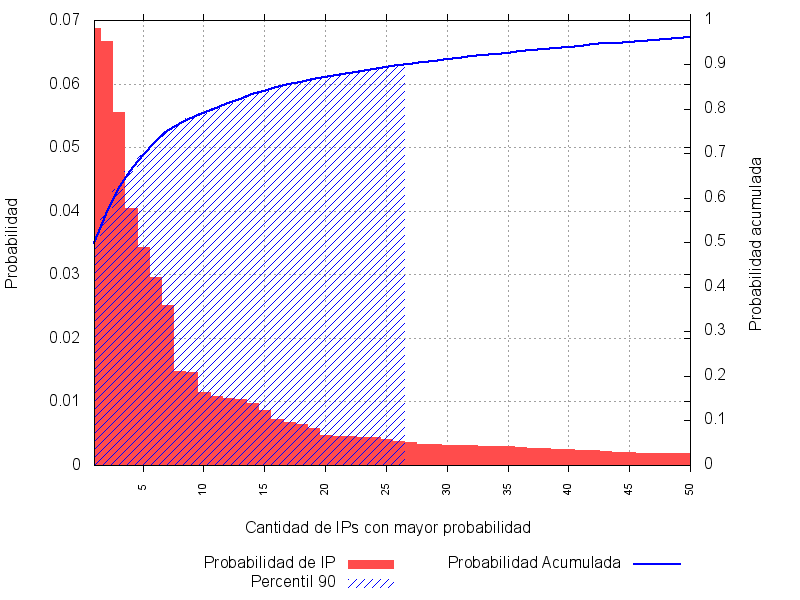
\includegraphics[width=0.5\textwidth]{escenario_1/vlan10/vlan10_src_bars_percentile90}
    \caption{Probabilidades VLAN \nameref{itm:vlan10} - Fuente Origen}
    \label{fig:vlan10_src_prob_per90}
\end{figure}

\par Observemos la figura \ref{fig:vlan10_src_prob_per90}. La misma se compone de 2
datos analizados sobre los resultados obtenidos. Por 
un lado, en el eje \textit{x} se tienen ordenadas, de mayor a menor, todas las IPs de la
fuente de datos seg\'un su probabilidad muestral. Los s\'imbolos en cuesti\'on (IPs) no
son expuestos en la gr\'afica a\'un ya que se solapar\'ian y har\'ian ilegible al gr\'afico.
En lugar de ello se expuso la cantidad de IPs que hay hasta cada punto marcado del eje%
\footnote{Donde dice \textit{5, 10, 15...}, se tienen de izquierda a derecha 5 IPs, 10
IPs, etc.}. 

\par En rojo tenemos la probabilidad muestral de los s\'imbolos (que por el orden impuesto
ir\'a obviamente decreciendo).

\par Por \'ultimo, en azul se puede ver la l\'inea de progreso de probabilidad acumulada.
En cada s\'imbolo del eje \textit{x}, la l\'inea azul nos indica cual es la sumatoria de
las probabilidades de todos los s\'imbolos (comenzando por el de mayor probabilidad) hasta
dicho punto.\\

\par As\'i pues, podemos observar que se llega al percentil 90 con tan solo los 27 s\'imbolos
de mayor probabilidad de la fuente. Es decir que menos del 0.01\% de los s\'imbolos aparecen
en nuestra fuente de datos con un 90\% de probabilidad.

\par Visto esto, ya nos interesa pasar a analizar de que IPs exactamente estamos hablando.
Como se vi\'o, en el an\'alisis lo m\'as determinante parecer\'ia ser aquellas IPs inclu\'idas
dentro del percentil 90. Las mismas se presentan a continuaci\'on:

\begin{figure}[!ht]
    \centering
    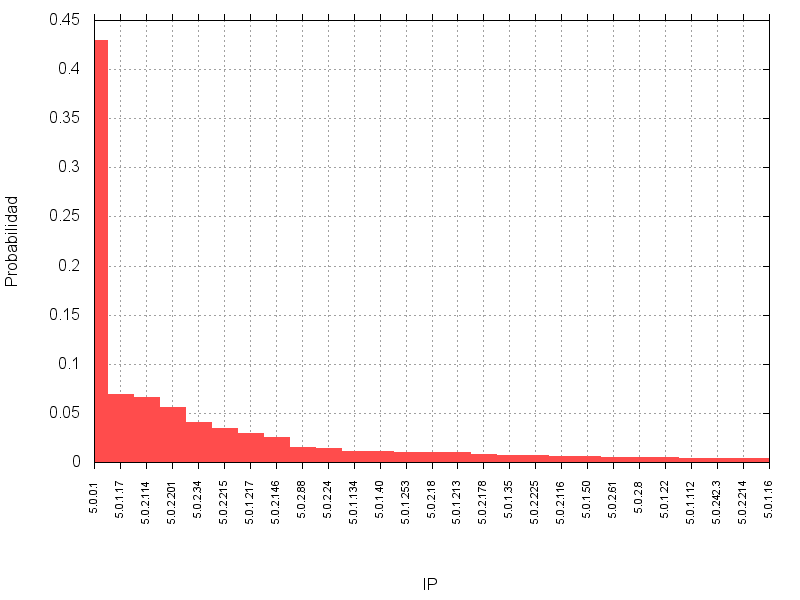
\includegraphics[width=0.5\textwidth]{escenario_1/vlan10/vlan10_src_probabilities_with_labels}
    \caption{IPs VLAN \nameref{itm:vlan10} - Fuente Origen}
    \label{fig:vlan10_src_prob_ips}
\end{figure}

\par Se puede observar en la figura \ref{fig:vlan10_src_prob_ips} que las primeras 6 IPs parecer\'ian
ser las principales de la red en enviar paquetes ARP (recordemos que estamos viendo los resultados
de la fuente de origen, es decir, los paquetes ARP cuya direcci\'on origen es la que fue
analizanda). Claramente estas IPs ya son candidatas a tener en cuenta al buscar nodos importantes
de nuestra red, ya que claramente est\'an env\'iando m\'as paquetes ARP que el resto, aunque el
motivo nos sea desconocido.


\subsubsection*{\underline{VLAN \nameref{itm:vlan10}: Fuente Destino}}\label{subsubsec:vlan10_dst}
\par Pasamos ahora a visualizar en la figura \ref{fig:vlan10_dst_prob_per90} los datos obtenidos
en la misma red, pero en la fuente destino, es decir, las IP's a las que fueron enviados los
paquetes ARP (o, dicho de otra forma, aquellos nodos a cuyos paquetes estaban destinados).

\begin{figure}[!ht]
    \centering
    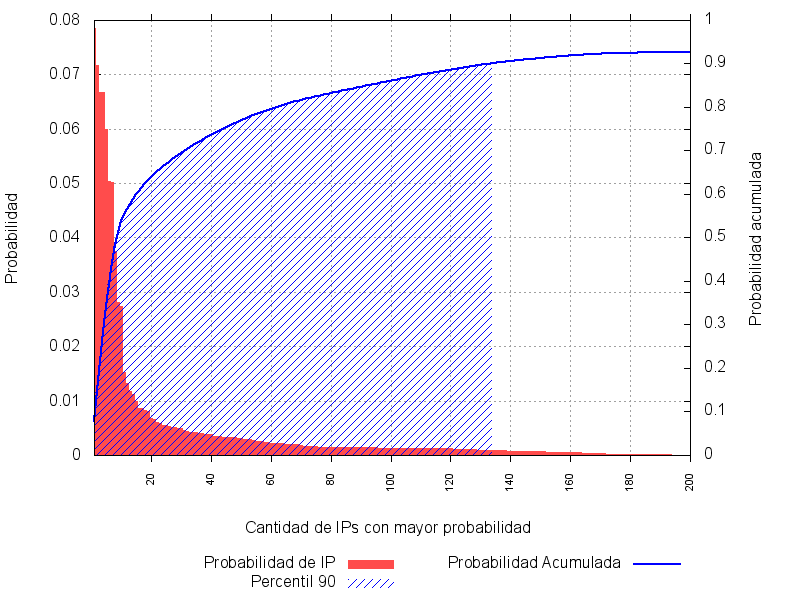
\includegraphics[width=0.5\textwidth]{escenario_1/vlan10/vlan10_dst_bars_percentile90}
    \caption{Probabilidades VLAN \nameref{itm:vlan10} - Fuente Destino}
    \label{fig:vlan10_dst_prob_per90}
\end{figure}

\par Nuevamente, se puede observar que se alcanza el percentil 90 de probabilidad de la
fuente con tan solo poco menos de 135 s\'imbolos (apr\'oximadamente representan un
0.03\% de la totalidad de IPs observadas en la fuente). Claramente, nos encontramos
nuevamente ante la situaci\'on de una red donde los destinos de los paquetes ARP
est\'an concentrados en unos pocos nodos. De hecho, no es casualidad que la cantidad
de personas que trabajan en esta red sean 70\footnote{Apr\'oximadamente}. Si se tienen
en cuenta algunos otras IPs que claramente no son de usuarios (posiblemente servidores)
y la posibilidad de usuarios con m\'as de una IP en la red\footnote{Interfases virtuales,
recordar que los \textit{hosts} de esta red son personal de un datacenter.}.

\par De hecho, si se observa con atenci\'on se podr\'a ver que en realidad, las primeras
50 IPs con mayor probabilidad conforman el percentil 80.

\par Observemos entonces, cuales son est\'as IPs que concentran la gran mayor\'ia
de la informaci\'on de nuestra fuente destino\footnote{En lugar de exponer la probabilidad
de las 135 IPs que componen el percentil 90, se tuvieron en cuenta las primeras 50 -percentil
80- dado que graficar tantos s\'imbolos har\'ia ilegible el gr\'afico y, a\'un m\'as importante
a\'un, a la hora de distinguir nodos importantes de la red, es muy probable que estos
se encuentren dentro de este percentil 80 que concentra tanta informaci\'on.}. Dicha informaci\'on
se presenta en la figura \ref{fig:vlan10_dst_prob_ips}.

\begin{figure}[!ht]
    \centering
    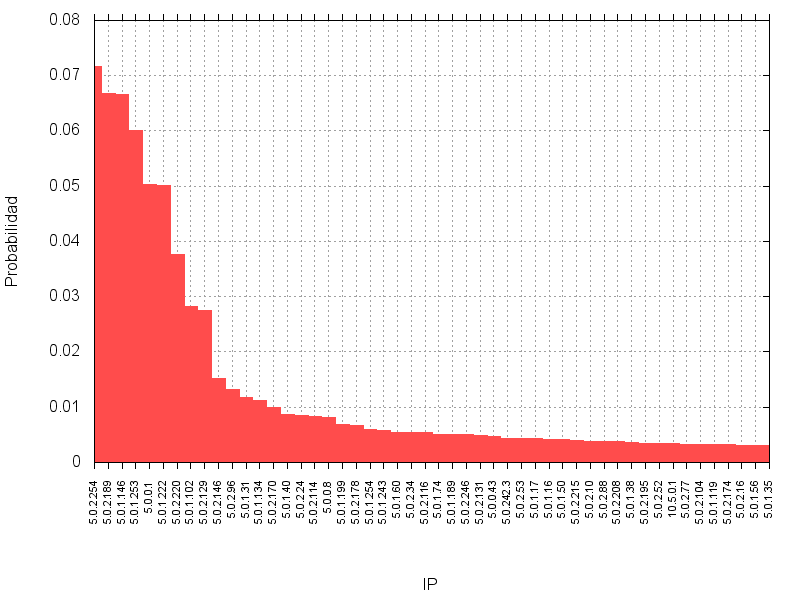
\includegraphics[width=0.5\textwidth]{escenario_1/vlan10/vlan10_dst_probabilities_with_labels}
    \caption{IPs VLAN \nameref{itm:vlan10} - Fuente Destino}
    \label{fig:vlan10_dst_prob_ips}
\end{figure}

\par En este \'ultimo gr\'afico podemos observar que dentro de las IPs que forman el percentil 80,
las 10 primeras IPs claramente componen la parte m\'as importante de la fuente. Es abrupta
la diferencia de las probabilidades, como se puede observar. As\'i pues, est\'as IPs que 
pareciesen ser muy solicitadas dentro de nuestra red, son claras candidatas a representar
nodos importantes.


\subsubsection*{\underline{VLAN \nameref{itm:vlan10}: Ambas Fuentes}}\label{subsubsec:vlan10_src_dst}
\par Toda la informaci\'on presentada hasta el momento nos permiti\'o identificar ciertas IPs
de la red (o s\'imbolos de la fuente) que seguramente son candidatos a representar algo notorio
o importante en la red \textit{sniffeada}. Pero a\'un no podemos llegar a conclusiones de la red,
dado que s\'olo obtivimos posibles IPs para dos fuentes distintas.

\par Para poder llegar a razonamientos coherentes sobre la red, debemos poder unir la informaci\'on
hasta ahora presentada de alguna manera. En primer instancia, es interesante observar las
relaciones entre las concentraciones de nodos de ambas fuentes (cantidad de IPs dentro del percentil
90/80 respecto de la totalidad de IPs de las fuentes) y las entrop\'ias:

\begin{table}[!h]
\centering
  \begin{tabular}{c c c c}
    Fuente& 
    Entrop\'ia & \begin{tabular}{@{}c@{}}Concentraci\'on \\ Percentil 90\end{tabular} 
    & \begin{tabular}{@{}c@{}}Concentraci\'on \\ Percentil 80\end{tabular}\\
    \hline\hline
    Origen & 3.87546 & 0.006\% & 0.002\%\\
    Destino & 6.50272 & 0.03\% & 0.015\%\\
    \hline\hline
    \end{tabular}
  \bigskip
  \caption{Concentraci\'on VLAN \nameref{itm:vlan10}}
  \label{tab:vlan10_concentracion}
\end{table}

\par Interesante como se ve el cuadro \ref{tab:vlan10_concentracion}, la \'unica nueva informaci\'on
que nos da es que claramente es que la incertidumbre de la fuente destino es mayor que la de la 
fuente destino. Es decir, mirando la concentraci\'on de los percentiles vemos que el 90\% de
probabilidades de la fuente destinoest\'a acumulado en un 0.03\% de los s\'imbolos de la fuente,
mientras que en la fuente origen est\'a a\'un m\'as concentrada. Esta concentraci\'on a nosotros,
dado nuestro objetivo, nos resulta \'util ya que nos permite reducir la cantidad de IPs que
probablemente cumplan con un rol importante dentro de la red.

\par As\'i pues llegamos a esta instancia con una reducci\'on de unas 160 IPs (entre ambas fuentes)%
\footnote{Se filtraron las IPs que componen los percentiles 90 de ambas fuentes.}
entre las cuales seguramente se encuentren los hosts importantes de la red \textit{sniffeada}. Se
presenta entonces a continuaci\'on un digrafo de la red entera, se\~nalando estas IPs candidatas.

\par Dado el gran tama\~no del \textit{dataset} (muchos nodos y muy denso en ejes\footnote{%
aproximadamente unos 4400 nodos con 12000 ejes}), se decidi\'o filtrar un poco m\'as los datasets
con alg\'un concepto intuitivo: si durante 77 horas de captura, un cierto par ordenado de direcciones
IP de un paquete ARP no se captur\'o m\'as de 500 veces, podemos asumir que dicho par no aporta
mucha informaci\'on, ya que se trata de informaci\'on espor\'adica que nos dan las fuentes de
datos.

\begin{figure*}[!t]
    \centering
    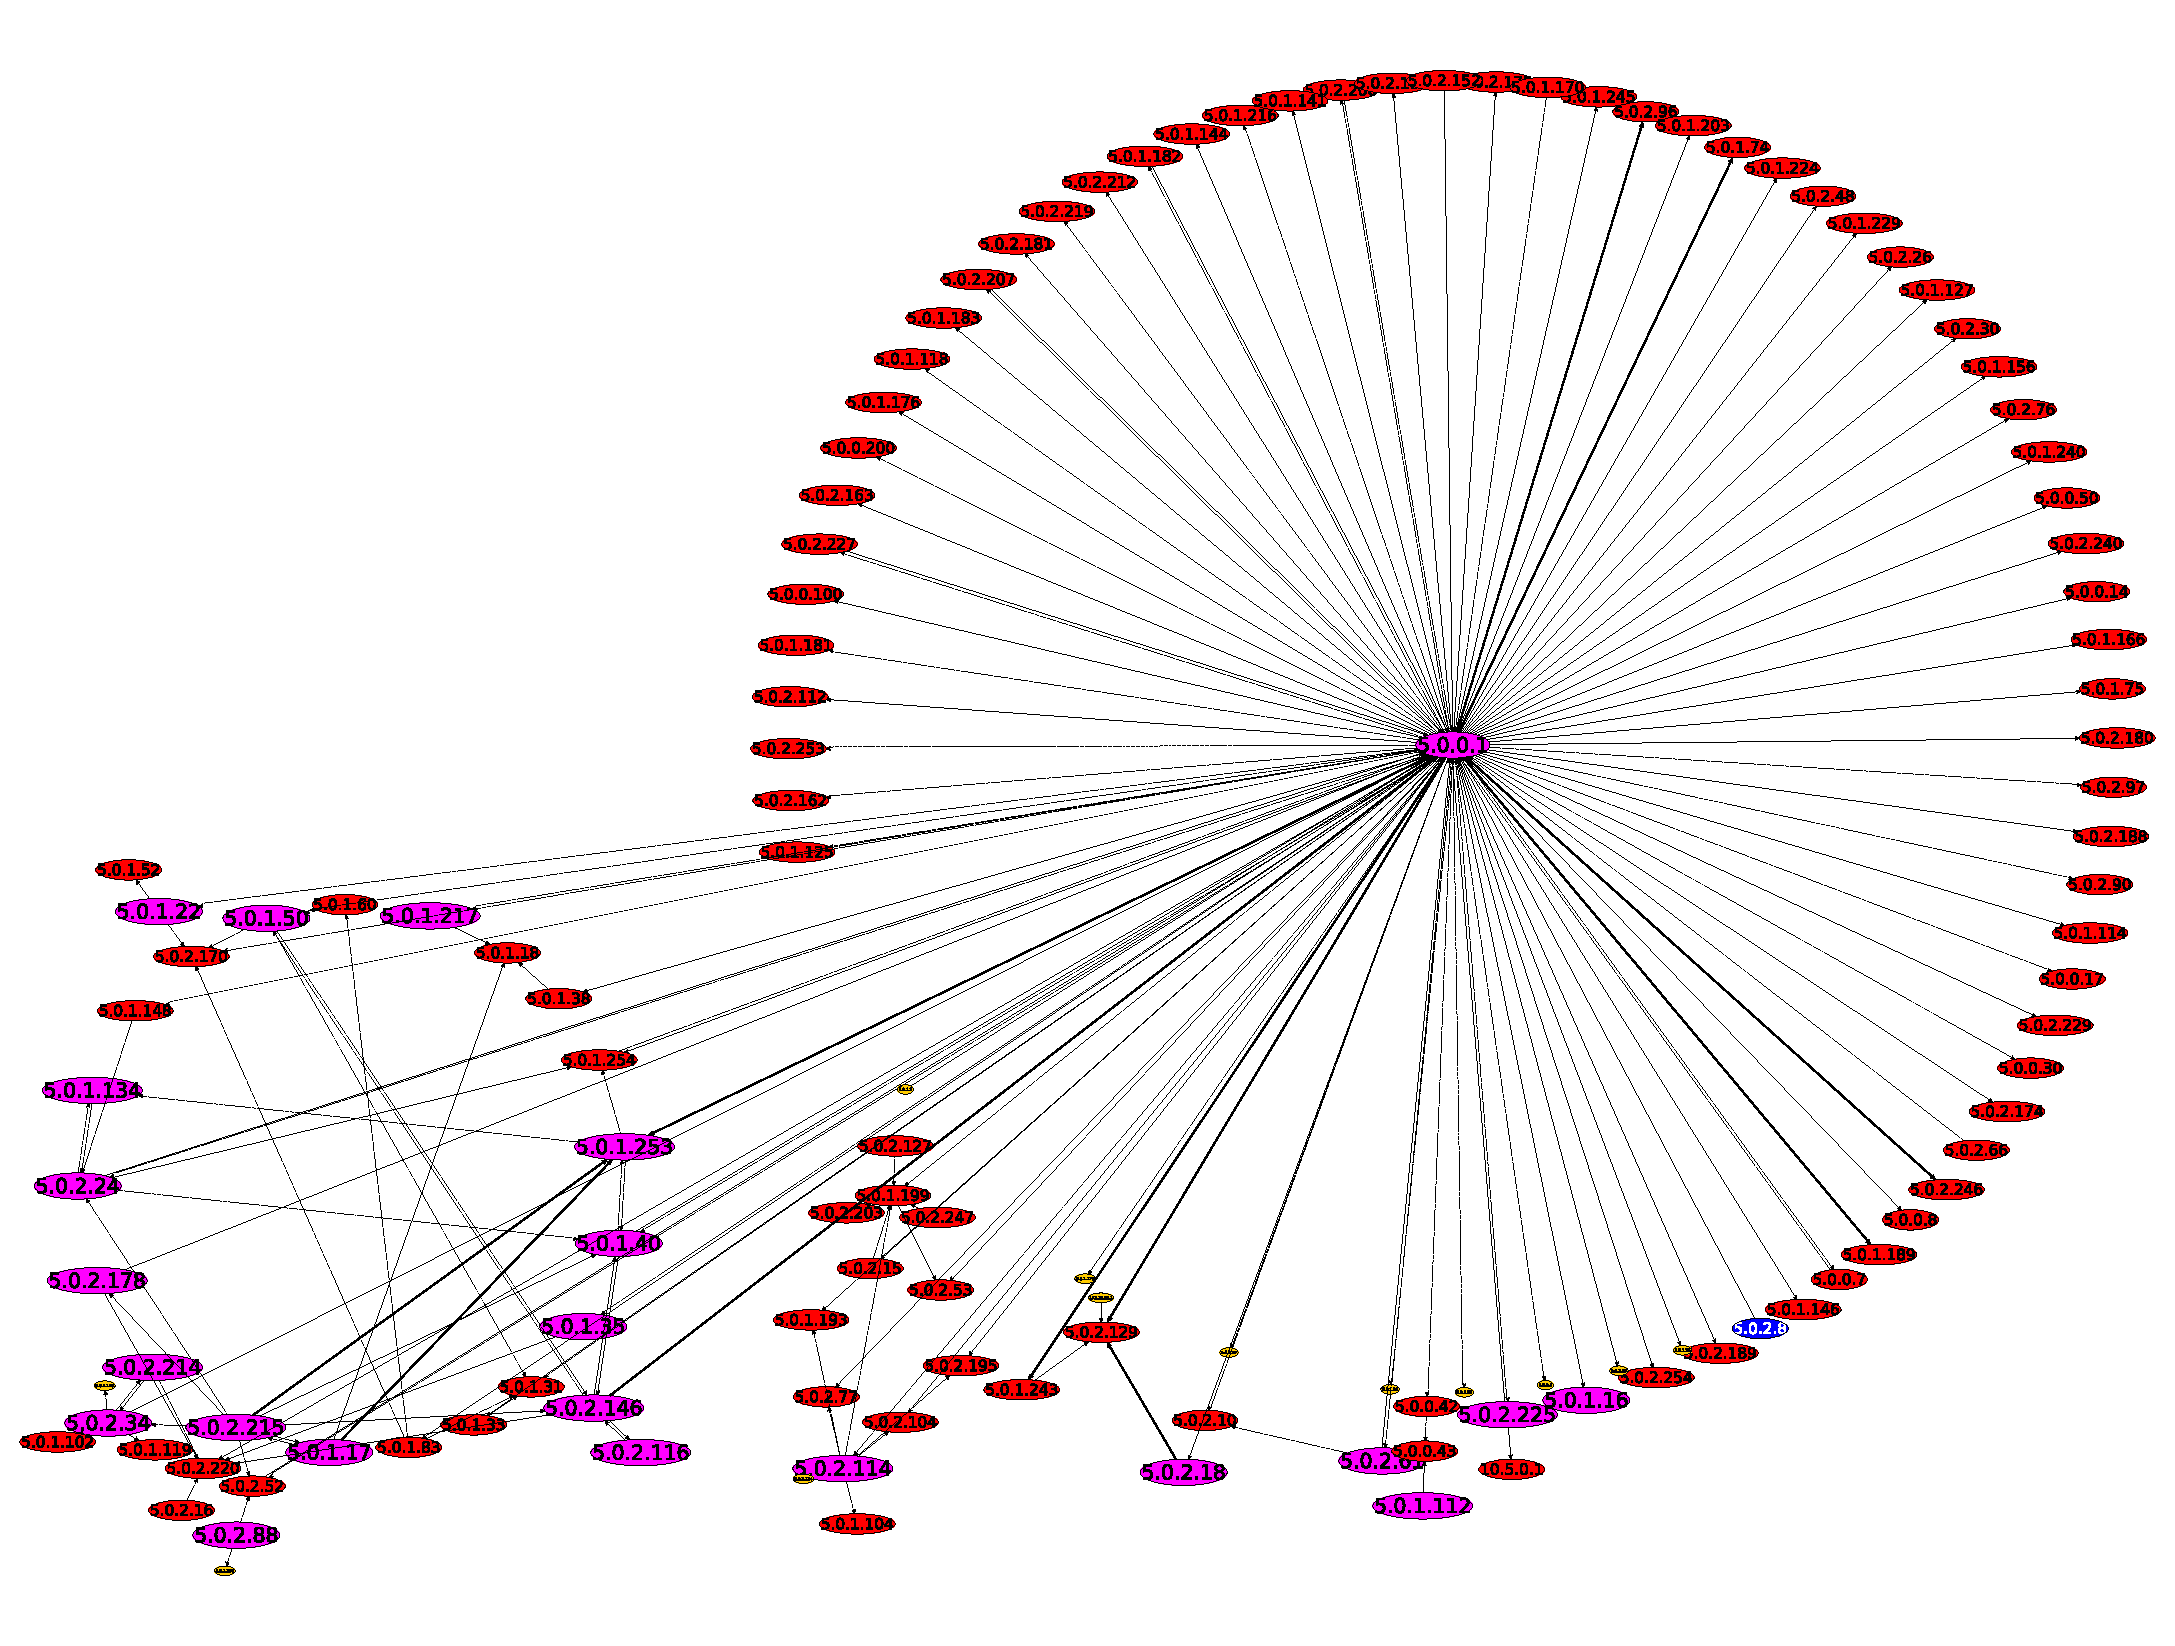
\includegraphics[width=\textwidth]{img/graph/escenario_1/vlan10/vlan10_500toEnd}
    \caption{Grafo VLAN \nameref{itm:vlan10}}
    \label{fig:vlan10_grafo}
\end{figure*}

\par En el grafo en cuesti\'on (figura \ref{fig:vlan10_grafo}) se colorearon los nodos
siguiendo la siguiente l\'ogica:

\begin{LaTeXdescription}
    \item[Rojo] Son los nodos que forman parte del percentil 90 de la fuente de
    direcciones de destino.\\

    \item[Azul] Son los nodos que forman parte del percentil 90 de la fuente de 
    direcciones de origen.\\

    \item[Violeta] Son las direcciones que forman parte del percentil 90 de ambas
    fuentes de direcciones.\\

\item[Ejes] Los ejes fuero formateados de manera tal que representacen el peso de los
    ejes. Es decir, la cantidad de paquetes con las direcciones origen y destino (o nodos)
    conectados por cada eje. A menor peso, la l\'inea ser\'a menos gruesa y hasta
    punteada, mientras que en el caso contrar\'i el eje ir\'a ganado grosor.\\

\end{LaTeXdescription}

\par Como se observa, el grafo parece indicar un flujo de paquetes ARP amplio desde
el nodo del centro hacia la gran mayor\'ia de los dem\'as nodos. En dicho nodo (que se
ampl\'ia en la figura \ref{fig:vlan10_grafo_centro}), puede notarse una afluencia
balanceada en cuanto a flechas entrando (direcci\'on destino) y flechas saliendo
(direcci\'on origen\footnote{No por nada dicha IP est\'a marcada con el color
\textit{violeta}.}). A su vez, si nos concentramos en los grosores de los ejes,
veremos que tambi\'en se encuentra enviando paquetes ARP con la misma (al menos
en una primera vista del gr\'afo) \textit{intensidad} con la que los recibe
por los demas nodos de la red.

\begin{figure}
    \centering
    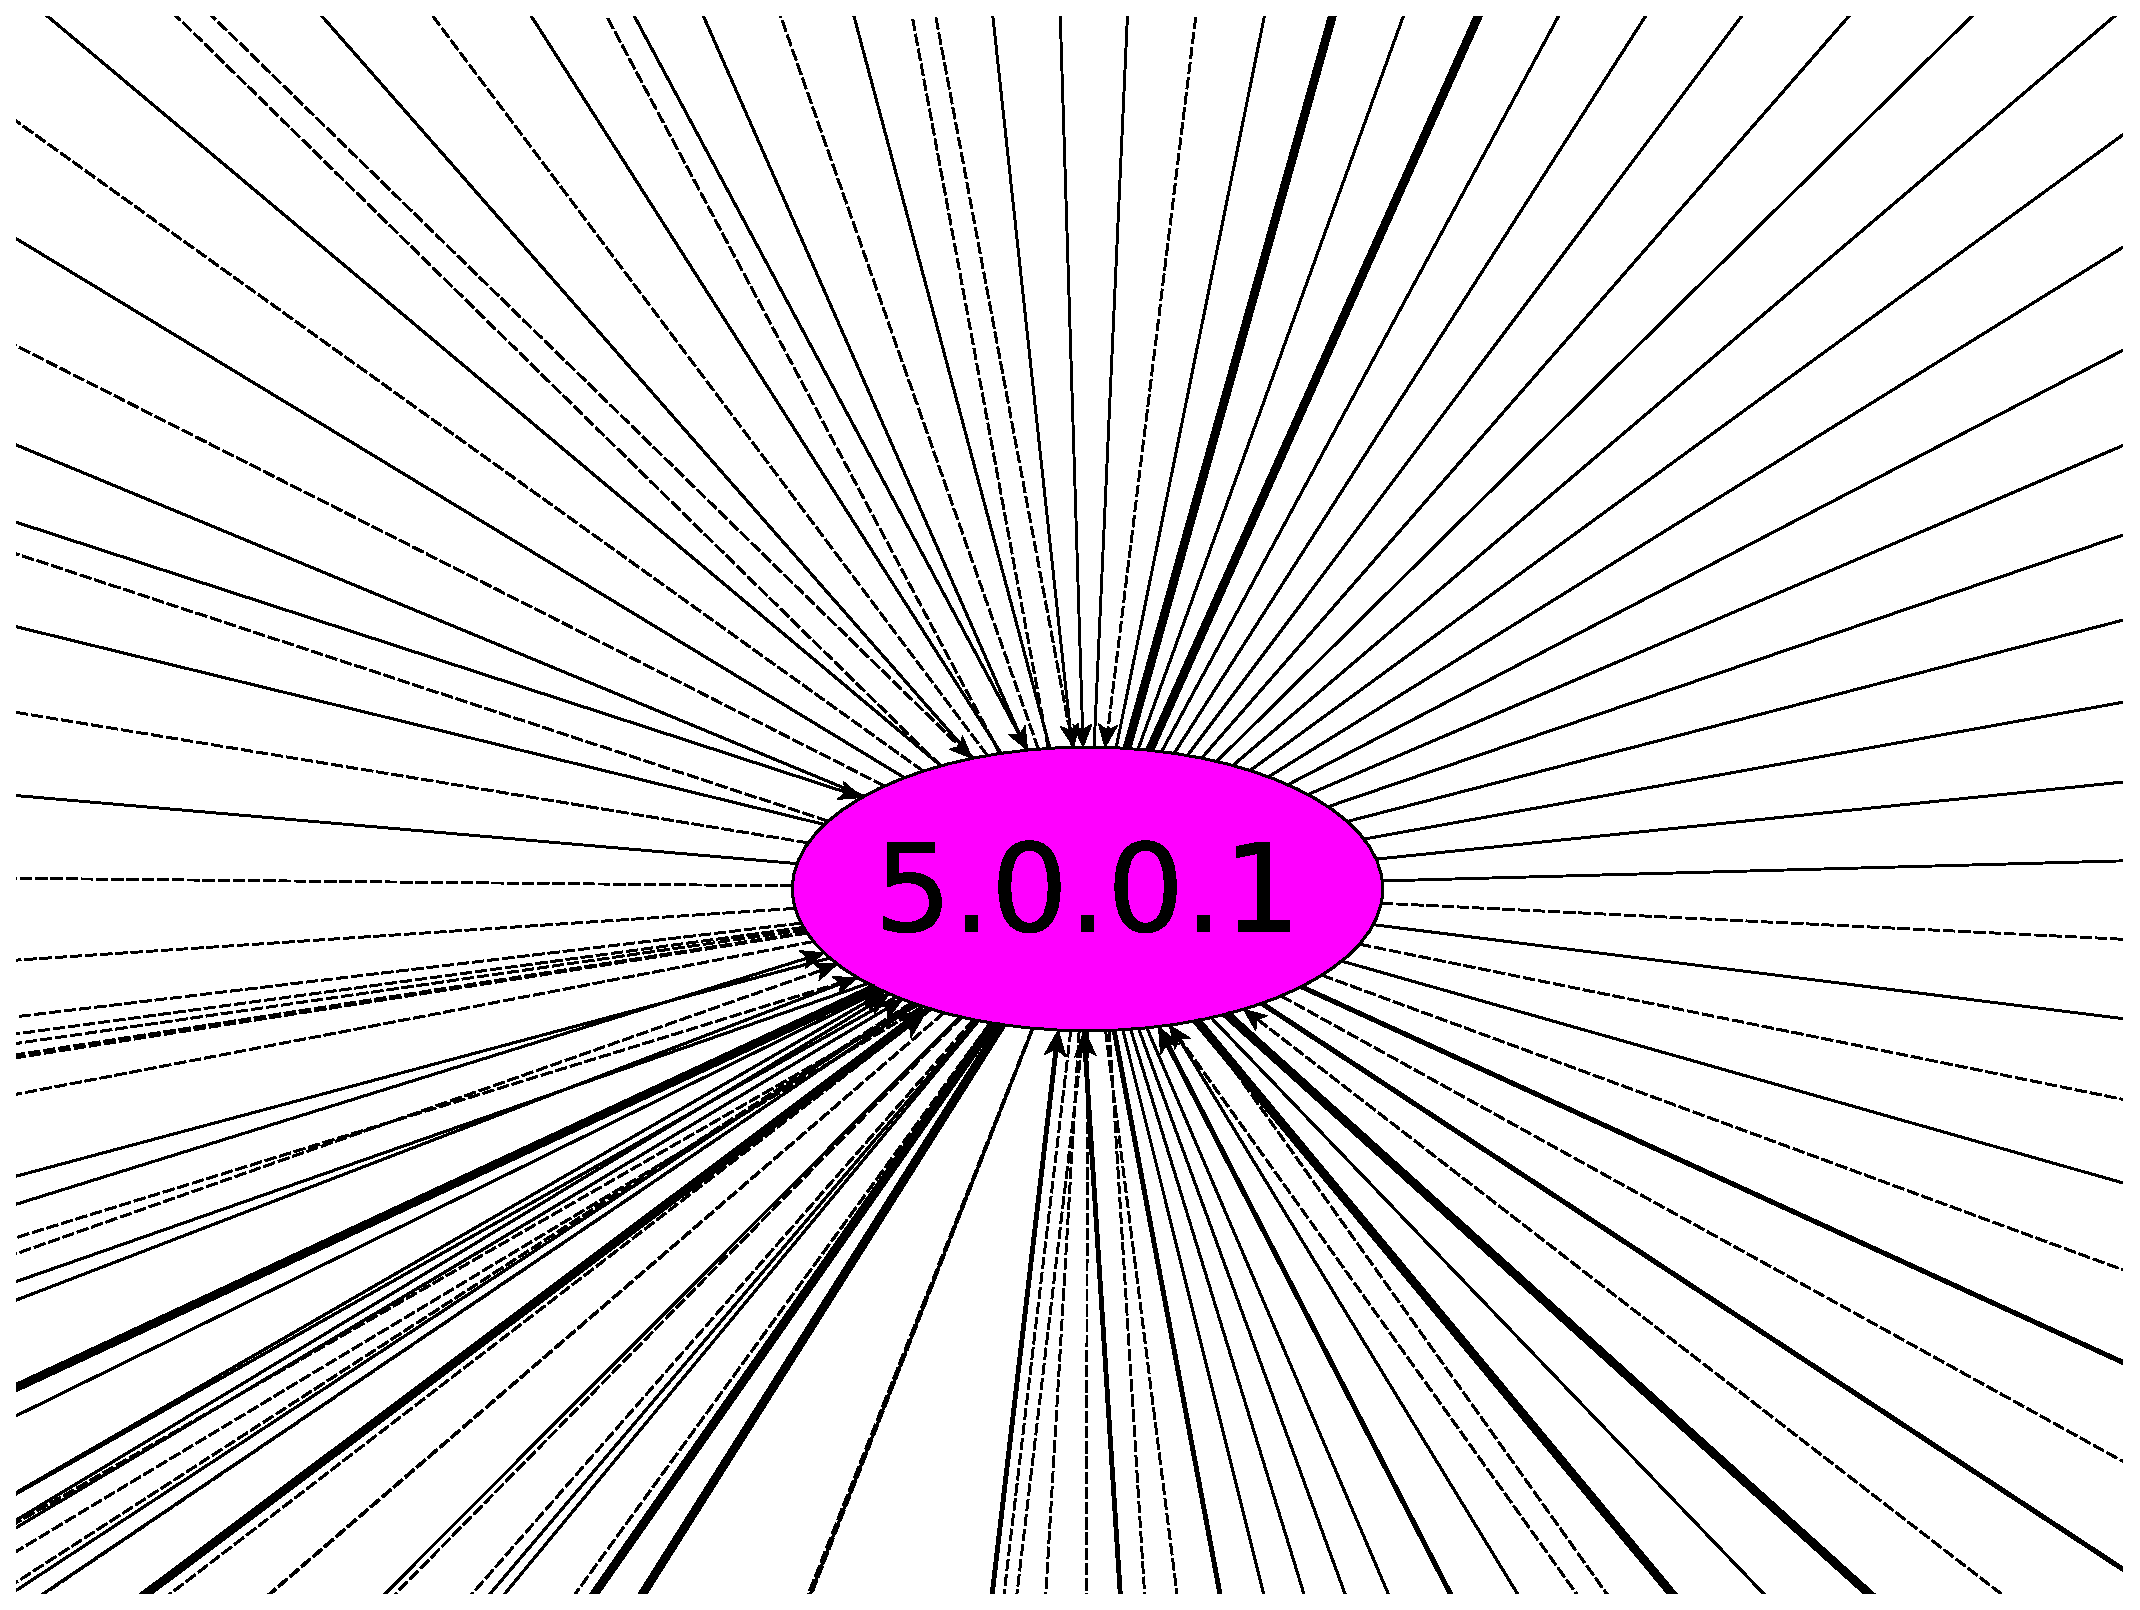
\includegraphics[width=0.5\textwidth]{img/graph/escenario_1/vlan10/vlan10_500toEnd_centro}
    \caption{Grafo VLAN \nameref{itm:vlan10} - Centro}
    \label{fig:vlan10_grafo_centro}
\end{figure}

\par Por \'ultimo, se observa una \textit{subregi\'on} en la zona izquierda donde varios
nodos parecer\'ieran estar env\'iandoso paquetes entre s\'i con bastante regularidad. A
\textit{prior\'i} estos parecer\'ian ser los nodos m\'as activos de la red durante el
transcurso de la semana. Se puede observar dicha zona en la figura \ref{fig:vlan10_grafo_inf}:

\begin{figure}
    \centering
    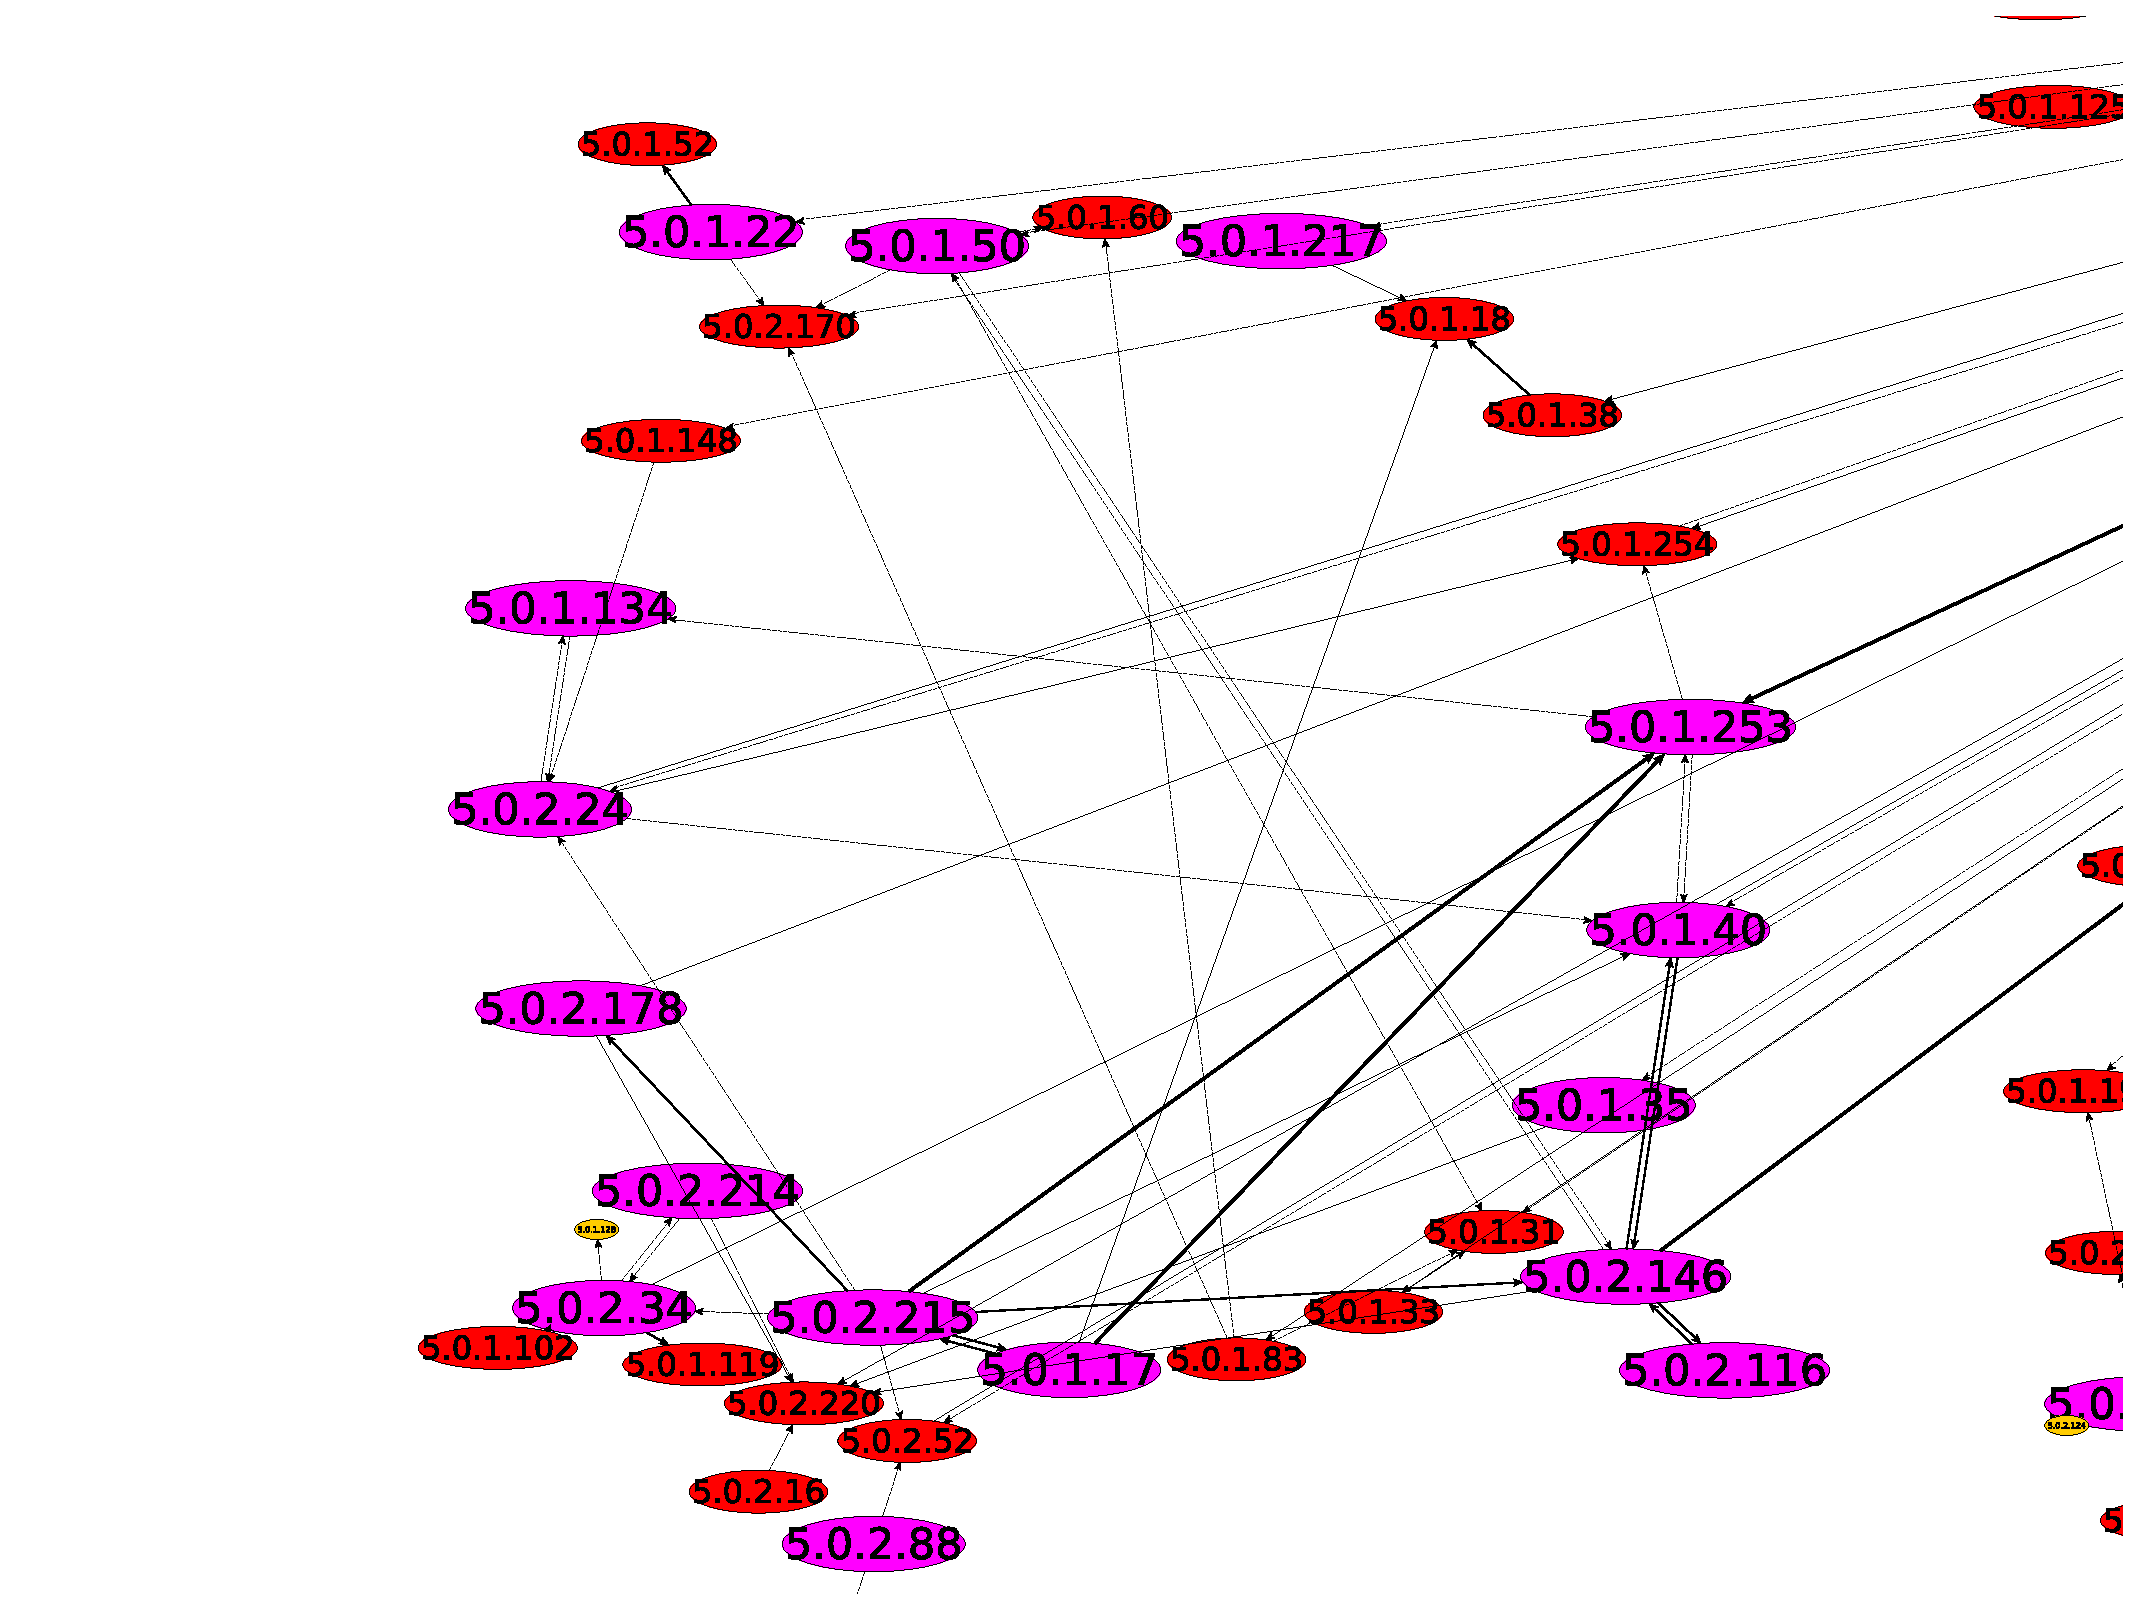
\includegraphics[width=0.5\textwidth]{img/graph/escenario_1/vlan10/vlan10_500toEnd_inf}
    \caption{Grafo VLAN \nameref{itm:vlan10} - Zona activa}
    \label{fig:vlan10_grafo_inf}
\end{figure}

\par En dicha regi\'on se puede ver que a pesar de la elevada actividad cruzada de paqutes
ARP entre los nodos, no hay nodo tan concurrido como el \textit{5.0.0.1}, el cual se
vi\'o en detalle hace tan solo unos momentos.


\subsubsection*{\underline{VLAN \nameref{itm:vlan10}: Conclusiones}}\label{subsubsec:vlan10_conclusiones}
\par Podemos concluir que claramente la direcci\'on \textit{5.0.0.1} es una
direcci\'on importante de la red. Se v\'io como aparece entre las direcciones con mayor
probabilidad tanto en la fuente de direcciones origen as\'i como destino, y se nota
en el grafo que es de entre los nodos con mayor probabilidad aquel que tiene la mayor
interacci\'on (en cuanto a cantidad) con el resto de los \textit{hosts} de la redes.

\par Este comportamiento es sumamente similar al comportamiento que tendr\'ia un equipo
encargado de \textit{routear} la red LAN hac\'ia otras redes, debido a la gran cantidad
de equipos que piden por su direcci\'on \textit{MAC} dentro de la VLAN.

\par Quiz\'as valga mencionar que de hecho hay otros nodos importantes en la red. Se
puede ver en la figura \ref{fig:vlan10_grafo_inf} como hay tres direcciones que se env\'ian
pedidos ARP con bastante frecuencia: \textit{5.0.1.253, 5.0.1.17, 5.0.2.15 y 5.0.246}.
No parecer\'ia ser casualidad que a todas estas IPs les haya correspondido el color
violeta en el grafo. Claramente la interaccion que tienen entre s\'i (m\'as all\'a de la
que tienen con los dem\'as nodos) parecer\'ia ser suficente, por las caracter\'isticas
de los ejes, para tener una alta probabilidad en ambas fuentes de s\'imbolos. Claramente
esto ser\'ia un dato de inter\'es para el administrador de la red, debido a que quiz\'as
estos equipos est\'an env\'iando paquetes broadcast en el dominio de colisi\'on sin
que haya necesidad.


    \subsubsection{VLAN de~\nameref{itm:vlan20}}
\par Habiendo ya pasado por el proceso de analizar una VLAN, nos encontramos en una
situaci\'on mucho m\'as concisa. En esta VLAN esperamos encontrar mucho menos tr\'afico
que en la anterior. Este razonamiento se debe a que esta es una red de servidores, con
lo cual se espera estar tomando datos de un ambiente mucho m\'as administrado, con
menos varianza de las terminales que se prenden/apaguan conectan/desconectan.

\par Estas caracter\'isticas del entorno nos hacen razonar tambi\'en que al ser
servidores con mucha menos manipulaci\'on, con las conexiones dentro de la LAN
seguramente mucho m\'as estables ya que nadie est\'a usando est\'as terminales
para \textit{salir} a internet o utilizandolas activamente con servicios que
deban salir a otra red salvo para la comunicaci\'on con los usuarios que se conectan
a los mismos.

\par As\'i pues, pasamos a los datos concretos de nuestro an\'alisis:

\begin{table}[!h]
\centering
  \begin{tabular}{c c}
    Fuente de Datos & Entrop\'ia \\
    \hline\hline
    Direcci\'on Origen & 3.01743 \\
    Direcci\'on Destino & 5.71059 \\
    \hline\hline
    \#IPs de las Fuentes & 2051\\
    \#Paquetes Capturados & 874806\\
    \hline
    \end{tabular}
  \bigskip
  \caption{Entrop\'ia VLAN \nameref{itm:vlan20}}
  \label{tab:vlan20_entropia}
\end{table}

\par Curiosamente, los resultados aqu\'i obtenidos nos dan una cantidad de paquetes
similar a la de la VLAN \nameref{itm:vlan10}. Compararemos estos resultados m\'as
adelante en la secci\'on \ref{sec:escenario1_supl}.


\subsubsection*{\underline{VLAN \nameref{itm:vlan20}: Fuente Origen}}\label{subsubsec:vlan20_src}
\par Pasamos ahora a visualizar las distintas probabilidades que nos d\'a esta fuente de
datos.

\begin{figure}[!ht]
    \centering
    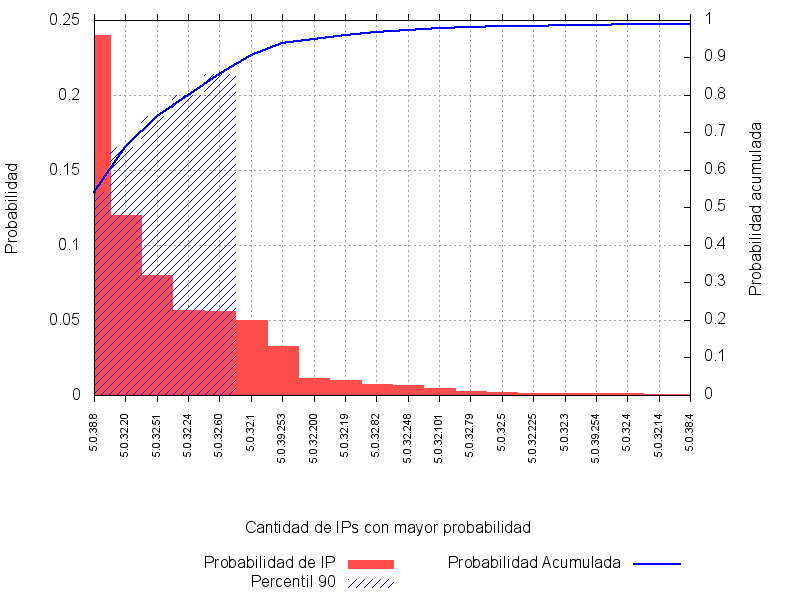
\includegraphics[width=0.5\textwidth]{escenario_1/vlan20/vlan20_src_bars_percentile90}
    \caption{Probabilidades VLAN \nameref{itm:vlan20} - Fuente Origen}
    \label{fig:vlan20_src_prob_per90}
\end{figure}

\par El resultado inmediato que se puede observar aqu\'i es la poca cantidad de IPs
requeridas para componer el percentil 90. Se ver\'a m\'as adelante que la concentraci\'on
de la informaci\'on en esta VLAN es mucho mayor que en el caso anterior. Se puede
ver con claridad que con tan solo con las 5 IPs de mayor probabilidad muestral se obtiene
la probabilidad acumulada del 90\% de la fuente. A\'un as\'i, vale la pena mencionar
nuevamente el dato expresado en la tabla \ref{tab:vlan20_entropia}, donde se puede
observar que la cantidad de IPs/S\'imbolos que nos di\'o la fuente fue extensamente
mayor.

\par Esto ya parecer\'ia estar indicando que en la red hay muy pocas terminales que
env\'ian paquetes ARP, al menos con una frecuencia comparable al caso de la VLAN
ya analizada.


\subsubsection*{\underline{VLAN \nameref{itm:vlan20}: Fuente Destino}}\label{subsubsec:vlan20_dst}
\par Veamos ahora que pasa con las otras terminales a la hora de responder a los
paquetes ARP. La pregunta que nos realizamos es si esas 5 terminales que acaparaban
todo el tr\'afico de env\'io de paquetes ARP es entre ellas, distribu\'ido entre
las dem\'as direcciones de la LAN o si simplemente son paquetes ARP env\'iados para
monitorear la red, en cuyo caso ir\'ian dirigidos a IPs inexistentes.

\begin{figure}[!ht]
    \centering
    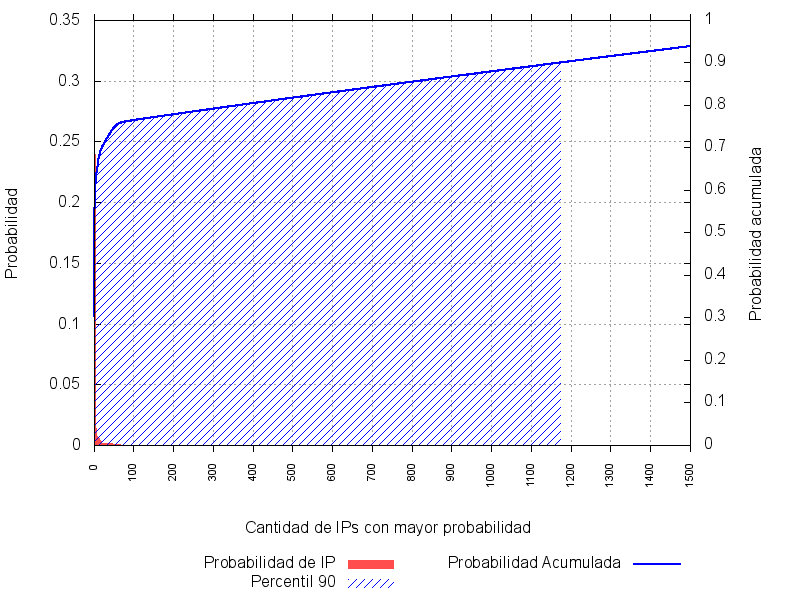
\includegraphics[width=0.5\textwidth]{escenario_1/vlan20/vlan20_dst_bars_percentile90}
    \caption{Probabilidades VLAN \nameref{itm:vlan20} - Fuente Destino}
    \label{fig:vlan20_dst_prob_per90}
\end{figure}

\par Notoriamente en este caso se puede observar como para alcanzar el percentil
90 se necesitan de algo menos que las 1200 direcciones IPs con mayor probabilidad
muestral. Ya esto nos da la pauta, a diferencia de lo que ve\'iamos observando
hasta este momento, de que en este entorno la fuente de direcciones destino
no est\'a tan concentrada. De hecho, parecer\'ia haber una \'unica IP que
es destinatario de m\'as de alg\'un paquete ARP, dandonos a entender que no es
una coincidencia impulsada, quiz\'as, por el tama\~no de la red el hecho de que
sea la \'unica IP de esta fuente de datos con una probabilidad no desestimable.

\begin{figure}[!ht]
    \centering
    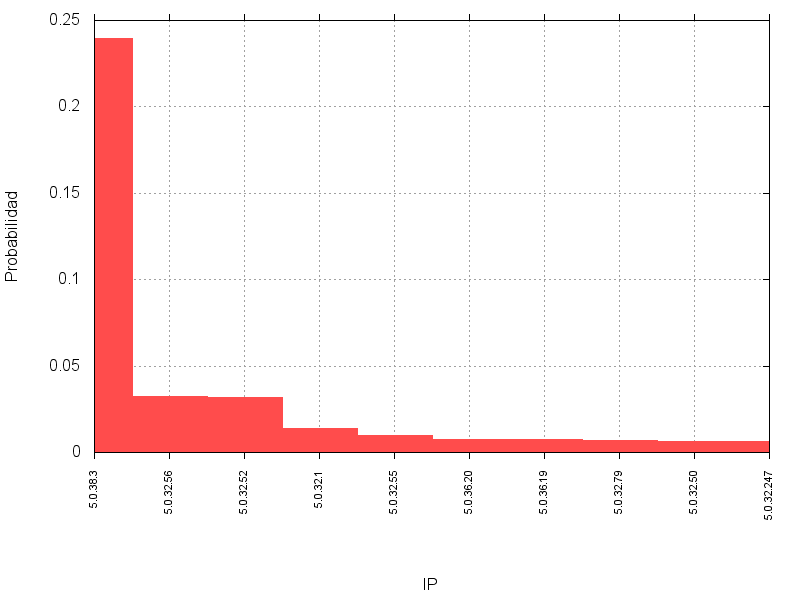
\includegraphics[width=0.5\textwidth]{escenario_1/vlan20/vlan20_dst_probabilities_with_labels}
    \caption{IPs VLAN \nameref{itm:vlan20} - Fuente Destino}
    \label{fig:vlan20_dst_prob_ips}
\end{figure}


\par Ya llegados a estas instancias, nos resulta interesante ver la siguiente tabla
y como contrasta con la del caso anterior:

\begin{table}[!h]
\centering
  \begin{tabular}{c c c c}
    Fuente& 
    Entrop\'ia & \begin{tabular}{@{}c@{}}Concentraci\'on \\ Percentil 90\end{tabular} 
    & \begin{tabular}{@{}c@{}}Concentraci\'on \\ Percentil 80\end{tabular}\\
    \hline\hline
    Origen & 3.01743 & 0.0024\% & 0.0014\%\\
    Destino & 5.71059 & 0.573\% & 0.183\%\\
    \hline\hline
    \end{tabular}
  \bigskip
  \caption{Concentraci\'on VLAN \nameref{itm:vlan10}}
  \label{tab:vlan20_concentracion}
\end{table}

\par Los n\'umeros aqu\'i ya nos est\'an diciendo mucho sobre la red. La baja entro\'ia
de la fuente de origen nos comunica que estamos ante una fuente de datos bastante
predecible. De hecho, esto luego se ve confirmado por la baja concentraci\'on de 
s\'imbolos que componen el percentil 90 y 80. Claramente con muy pocas direcciones
ya se tiene una gran probabilidad acumulada de la fuente, sabiendo entonces que seguramente,
si hay un paquete ARP, poder indicar 6 direcciones sobre 2051 con una probabilidad muestral
del 90\%.

\par Por lo contrar\'io, la fuente destino es ya bastante m\'as impredecible. Si bien su
entrop\'ia no es alta (al menos comparada con los otros casos ya expuestos), vemos una
concentraci\'on considerable (respecto de la fuente de origen) en el percentil 90. Pero
observando la figura \ref{fig:vlan20_dst_prob_ips}, podemos ver que en realidad, hay
una direcci\'on particular que tiene casi un 25\% de probabilida de surgir de esta fuente, pero
ocurre que todas las dem\'as direcciones tienen una probabilidad muy baja. Por lo tanto,
sabemos que existe una \'unica IP en realidad que podr\'ia llegar a ser esperada con cierta
justificaci\'on, pero es todo lo que podemos decir de este dominio de colisi\'on.


\subsubsection*{\underline{VLAN \nameref{itm:vlan20}: Ambas Fuentes}}\label{subsubsec:vlan20_src_dst}
\par A diferencia de la VLAN de \nameref{itm:vlan10}, aqu\'i ya pudimos obtener varios
resultados interesantes y bastante expl\'icitos sobre el comportamiento de las fuentes
de informaci\'on analizados. No obstante, es interesante verificar como se compone
el gr\'afo de esta fuente, en parte para confirmar las hip\'otesis planteadas sobre
el funcionamiento de la red y tambi\'en para verificar si no hay alg\'un dato
o caractar\'istica que no pueda ser visto mediante las probabilidades ya expuestas.

\par En el grafo que se presenta a continuaci\'on se utilizan las mismas reglas de coloreo
y de grosores ya explicadas en la secci\'on \ref{subsubsec:vlan10_src_dst}. Al igual
que en el caso anterior, desestimamos aquellos ejes que no tuvieran un peso
superior a 70 (en lugar de 500 del caso anterior, ya que esta VLAN contiene muchas
menos direcciones IP y mucho menos tr\'afico ARP tambi\'en). La justificaci\'on subyacente
es la misma que antes: luego de 77 horas de captura de paquetes, si un servidor
trata de obtener espor\'adicamente la \textit{MAC} de otra terminal, es un dato
que no nos suma a la topolog\'ia que tratamos de descubrir (ya que agregar\'a ejes
que ocurren con muy poca probabilidad).

\begin{figure*}[!t]
    \centering
    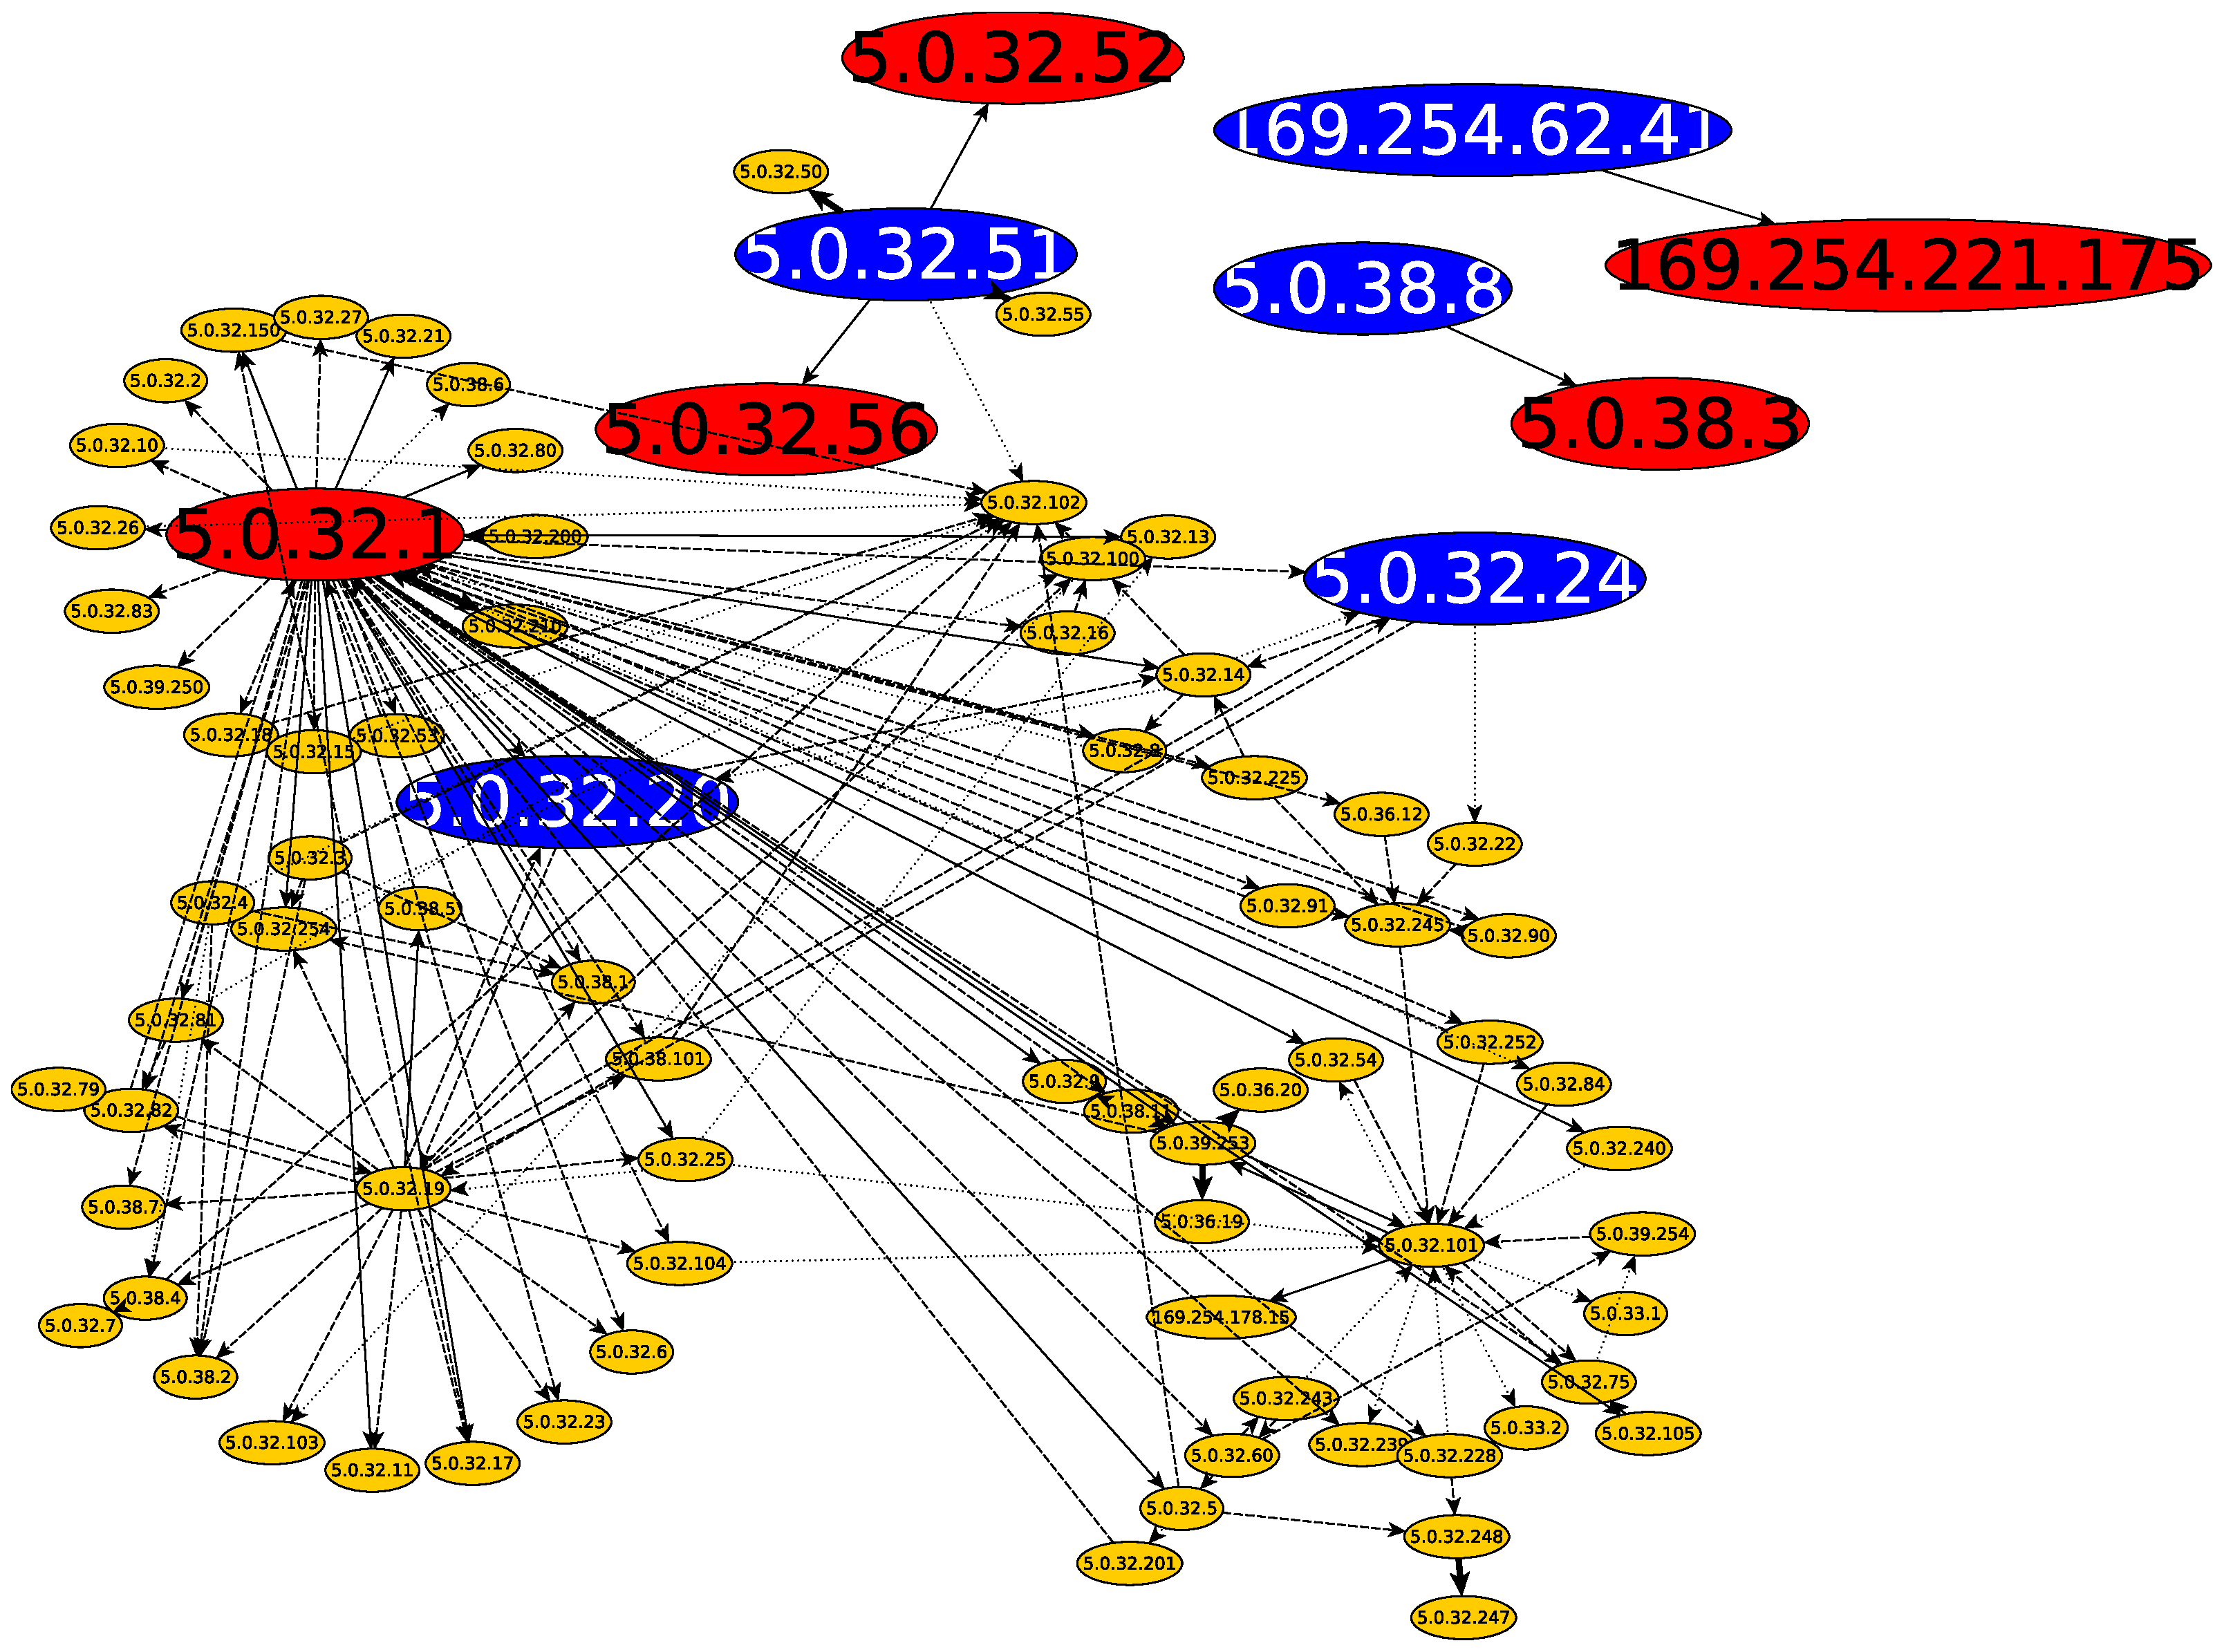
\includegraphics[width=\textwidth]{img/graph/escenario_1/vlan20/vlan20_70toEnd}
    \caption{Grafo VLAN \nameref{itm:vlan20}}
    \label{fig:vlan20_grafo}
\end{figure*}

\par En la figura \ref{fig:vlan20_grafo} se pueden observar ciertas cosas esperables
como otras que no tanto.

\par En primer lugar, salvo los nodos inclu\'idos en los percentiles 90, no pareciese
haber pedidos de resoluci\'on de \textit{MAC}\footnote{Abuso de notaci\'on.} entre
los hosts con poca probabilidad. Como posibles excepciones a esto se pueden ver las
IPs \textit{5.0.32.101, 5.0.32.19 y 5.0.32.102}. Si bien hay algunas otras con menor
afluencia que estas tres, hay que mencionar que ya en estas direcciones que mencionamos,
los ejes est\'an representados con flechas punteadas (es decir, no hay un pedido realmente
consistente de la \textit{MAC} de estos hosts).

\par Siguiendo con esta l\'inea de razonamiento, podemos ver que los ejes que denotan
"conexiones" consistentes entre servidores son pocos (lo cual es coherente con la
informaci\'on analizada hasta aqu\'i). Destacan por ah\'i algunas relaciones entre
la IP \textit{5.0.32.1}, claramente consultada por casi todos los nodos de la red (%
lo cual nos lleva a intu\'ir que este es un nodo importante de la red, ya que casi
todos en alg\'un momento durante la semana requieren poder conectarse a \'el) y 
los pedidos constantes de la \textit{5.0.32.51} para las direcciones \textit{5.0.32.56,
5.0.32.52, 5.0.32.50 y 5.0.32.55}\footnote{Estas \'ultimas dos ni siquiera forman
parte de uno de los percentiles 90}. Claramente aqu\'i, si consideramos que la
\textit{5.0.32.1} es posiblemente el \textit{gateway} de la red, nos encontramos
con 4 interfases de red que trabajan constantemente codo a codo (lo cual tambi\'en
explicar\'ia lo cercano de sus direcciones, aunque esto es simplemente algo que
se suele hacer en los \'ambitos de administraci\'on de servidores\footnote{Y \'unicamente
cuando los servidores son reci\'en instalados y hay IPs libres en la red.}).

\par Notoriamente, un resultado que no esper\'abamos encontrar es ver que parece
ser la \textit{5.0.32.1} el gateway de la red en lugar de la \textit{5.0.38.3} o la
\textit{5.0.38.8}, que son las direcciones con mayor probabilidad en ambas fuentes de informaci\'on.
Esto sorprende, pero como se ha dicho anteriormente, estando en una red de servidores no se espera
que estos deban de comunicarse con otras redes tan seguido como por ah\'i lo hacen
las terminales de otras redes (principalmeente porque los servidores se comunican
entre s\'i para la gran parte de sus tareas\footnote{Los servidores una vez instalados
no se actualizan jam\'as. \textit{If ain't broken, don't fix it}. Manual b\'asico
del administrador de servidores.}).

\par Prosiguiendo, se nota que el tr\'afico entre la \textit{5.0.38.8} hacia
la \textit{5.0.38.3} es constante, ya que esta \'ultima tiene la probabilidad
m\'as alta de la fuente de destino y la primera la tiene en la fuente de origen. Claramente
estas dos terminales deben estar proveyendo alg\'un tipo de servicio, o utilizando
una el servicio de la otra, constantemente, ya que sus probabilidades son
notoriamente mayores que la del resto de las IPs.


\subsubsection*{\underline{VLAN \nameref{itm:vlan20}: Conclusiones}}\label{subsubsec:vlan20_conclusiones}
\par Lo m\'as interesante que se puede ver en esta red es que las probabilidades
de los direcciones IP, tanto de la fuente de origen como destino, no son
necesariamente sim\'etricas. Aprendimos esta diferencia con este caso, que a
a diferencia del caso anterior, nos mostr\'o que se puede tener un percentil 90
muy concentrado e muy pocas IPs y en la misma linea, la fuente opuesta ser
completamente lo contrario.

\par En la misma l\'inea, observa como no siempre habr\'a una direcci\'on
m\'as requerida por los dem\'as por el simple hecho de actuar de \textit{gateway}
para comunicarse con otras redes\footnote{Al menos, asumimos que en la mayor\'ia
de estas redes hay una direcci\'on que realiza esta tarea, cuyo comportamiento
parecer\'ia ser identificable facilmente, ya que deber\'ia ser requerido por
las dem\'as terminales con bastante frecuendia. Cosa que este entorno demostr\'o
que no siempre es as\'i.} no ser\'a la IP con mayor probabilidad. La comunicaci\'on
entre terminales de la misma red no se da a nivel de \textit{routeo}, por lo
cual puede haber muchos paquetes ARP entre otras terminales que, por ejemplo,
compartan servicios (http,ftp,nfs,etc) dentro de la LAN, generando mucho
tr\'afico sin necesidad de salir de la red local.


    \subsubsection{VLAN de~\nameref{itm:vlan40}}
\par Para continuar con el estudio de las fuentes de paquetes ARP en distintas redes,
propusimos \textit{sniffear} una red local no tan convencional como lo son las
redes de computadoras ethernet o \textit{Wi-Fi}. Por ello trabajamos sobre una
red de telefon\'ia IP.

\par En esta redes los protocolos utilizados son los mismos que se vienen viendo
durante todo el trabajo. Aunque claramente, al ser los dispositivos tel\'efonos,
se espera ver un comportamiento distinto. En particular, este comportamiento
depender\'a de los dispositivos que componen a la red: los tel\'efonos IP.

\par Es de conocimiento en el \'area donde se ha realizado la tarea de recolecci\'on
datos, que estos dispositivos suelen tener comportamientos inesperados. De hecho,
en varios casos experimentados se observo como ciertas impresoras IP realizaban
env\'ios de paquetes \textit{broadcast} sin cesar, saturando el medio compartido
y, en la jerga informal, \textit{tirar abajo la red.}

\par Comenzamos como ven\'imos haciendo hasta ahora, con la entrop\'ia y los
datos generales de los datos obtenidos:

\begin{table}[!h]
\centering
  \begin{tabular}{c c}
    Fuente de Datos & Entrop\'ia \\
    \hline\hline
    Direcci\'on Origen & 0.0218949 \\
    Direcci\'on Destino & 5.20051 \\
    \hline\hline
    \#IPs de las Fuentes & 47\\
    \#Paquetes Capturados & 40\,034 \\
    \hline
    \end{tabular}
  \bigskip
  \caption{Entrop\'ia VLAN \nameref{itm:vlan40}}
  \label{tab:vlan40_entropia}
\end{table}

\par Ya de inmediato podemos ver que nos encontramos ante una LAN distinta. La entrop\'ia
de la fuente de origen es muy baja, lo cual nos da la pauta de que saber quienes son
los dispositivos que env\'ian paquetes ARP no deber\'ia ser algo incierto, sino todo
lo contrario.

\par Esto es entendible debido a que se ve que nos encontramos ante una red "peque\~na",
al menos considerando los 2 casos anteriores.


\subsubsection*{\underline{VLAN \nameref{itm:vlan40}: Fuente Origen}}\label{subsubsec:vlan40_src}
\par Veamos entonces como son las probabilidades de estas direcciones.

\begin{figure}[!ht]
    \centering
    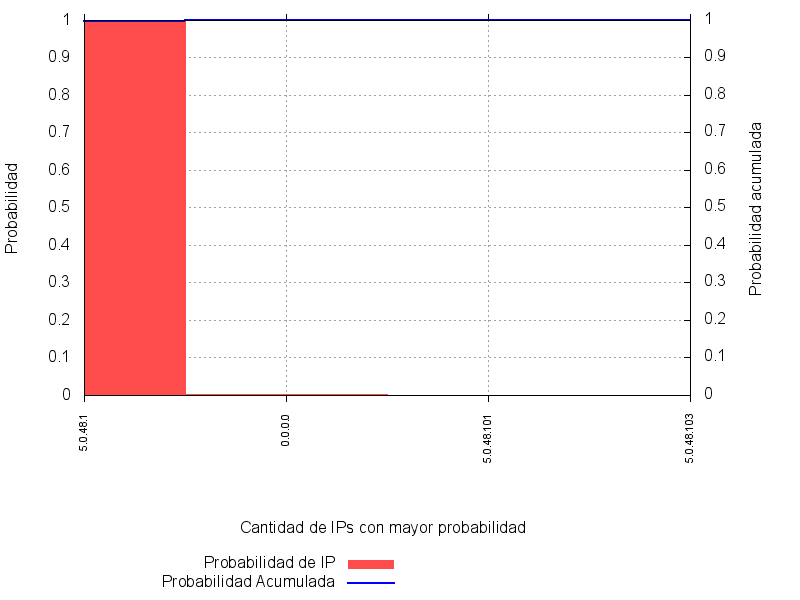
\includegraphics[width=0.5\textwidth]{escenario_1/vlan40/vlan40_src_bars_percentile90}
    \caption{Probabilidades VLAN \nameref{itm:vlan40} - Fuente Origen}
    \label{fig:vlan40_src_prob_per90}
\end{figure}

\par Como se puede observar en la figura \ref{fig:vlan40_src_prob_per90}, ni siquiera
es necesario trabajar con el percentil 90. Hay tan pocas IPs, y -aparentemente- los
tel\'efonos no indundan la VLAN con paquetes de ARP. Esto podr\'ia deberse a muchos
distintos factores, como la configuraci\'on de estos y el software que utilizan%
\footnote{Es porbable que muchos tel\'efonos no requieran de enviar paquetes ARP ya
que por ah\'i memorizan la \textit{MAC} de la \textit{PBX} en caso de estar esta
en su LAN.}.

\par En cualquier caso, conviene observar que ocurre con la fuente de destino.
De momento lo \'unico que podemos decir es que los tel\'efonos no parecen
env\'iar demasiados paquetes ARP en la red.


\subsubsection*{\underline{VLAN \nameref{itm:vlan40}: Fuente Destino}}\label{subsubsec:vlan40_dst}

\begin{figure}[!ht]
    \centering
    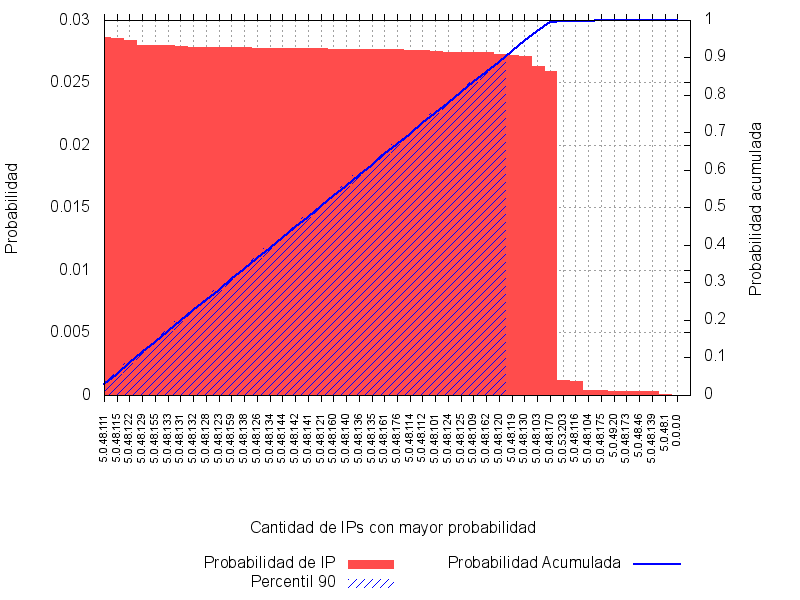
\includegraphics[width=0.5\textwidth]{escenario_1/vlan40/vlan40_dst_bars_percentile90}
    \caption{Probabilidades VLAN \nameref{itm:vlan40} - Fuente Destino}
    \label{fig:vlan40_dst_prob_per90}
\end{figure}

\par Nuevamente nos encontramos con un caso impensado\footnote{Para el estudiante al menos}
en un principio. Se puede observar en la figura \ref{fig:vlan40_dst_prob_per90} que al
contrario de lo que ocurre  en la fuente de origen, en la red de telefon\'ia IP los dispositivos
tienen una distribuci\'on de la probabilidad aproximadamente equiprobable. Es decir, cada
tel\'efono, en su mayor\'ia, tiene la misma probabilidad que el resto de aparecer como
un mensaje devuelto por la fuente de informaci\'on que se est\'a estudiando.

\par Esto puede ser observado no solamente por las barras de probabilidad, sino por el
crecimiento lineal del percentil90, que no sindica que las probabilidades de cada
IP est\'an aportando aproximadamente lo mismo al percentil.

\par Es esperable ver entonces que la concentraci\'on de la probabilidad deber\'ia ser
un n\'umero que se acerque a 1 (al menos, que se acerque mucho m\'as que los casos
hasta ahora estudiados). Esto se debe a que vemos que el percentil 90 se
alcanza casi teniendo en cuenta las probabilidades de todas las IPs.

\begin{table}[!h]
\centering
  \begin{tabular}{c c c c}
    Fuente& 
    Entrop\'ia & \begin{tabular}{@{}c@{}}Concentraci\'on \\ Percentil 90\end{tabular} 
    & \begin{tabular}{@{}c@{}}Concentraci\'on \\ Percentil 80\end{tabular}\\
    \hline\hline
    Origen & 0.0218949 & 0.0021\% & 0.0021\%\\
    Destino & 5.20051 & 0.681\% & 0.553\%\\
    \hline\hline
    \end{tabular}
  \bigskip
  \caption{Concentraci\'on VLAN \nameref{itm:vlan40}}
  \label{tab:vlan40_concentracion}
\end{table}

\par Efectivamente, lo que se ven\'ia reflejando ahora tambi\'en se demuestra con los
valores del cuadro \ref{tab:vlan40_concentracion}. Vemos como la entrop\'ia de la fuente
de origen es muy baja, debido a que casi toda la probabilidad de la fuente se concentra
en una \'unica direcci\'on IP (ver figura \ref{fig:vlan40_src_prob_per90}), teniendo
al mismo tiempo una concentraci\'on muy baja del percentil 90 (al fin y al cabo, es
s\'olo una IP la que acumula todo).

\par Por el otro lado, vemos que como fuente de destino, nos encontramos con una concentraci\'on
del percentil m\'as alta que en casos anteriores. El hecho de que la probabilidad
sea casi equiprobable entre todos los s\'imbolos de la fuente nos da una entrop\'ia
relativamente alta para la cantidad de IPs que se tienen en la fuente (47). Esto se
debe a que al ser equiprobable\footnote{Apr\'oximadamente} el espacio de s\'imbolos
de la fuente, hay una gran incertidumbre que no nos permite asegurar con una buena
base estad\'istica sobre quienes son los datos m\'as probables que nos dar\'a la
fuente.

\subsubsection*{\underline{VLAN \nameref{itm:vlan40}: Ambas Fuentes}}\label{subsubsec:vlan40_src_dst}
\par Dado que estamos en una red chica y, aparentemente poco densa, sumado a la
probabilidad concentrada de la fuente de origen y la distribu\'ida de la fuente destino,
nos da a entender que nos encontraremos con una topolog\'ia donde todos se comunican
con la IP \textit{5.0.48.1}\footnote{\nameref{fig:vlan40_src_prob_per90}.}.

\begin{figure}[ht]
    \centering
    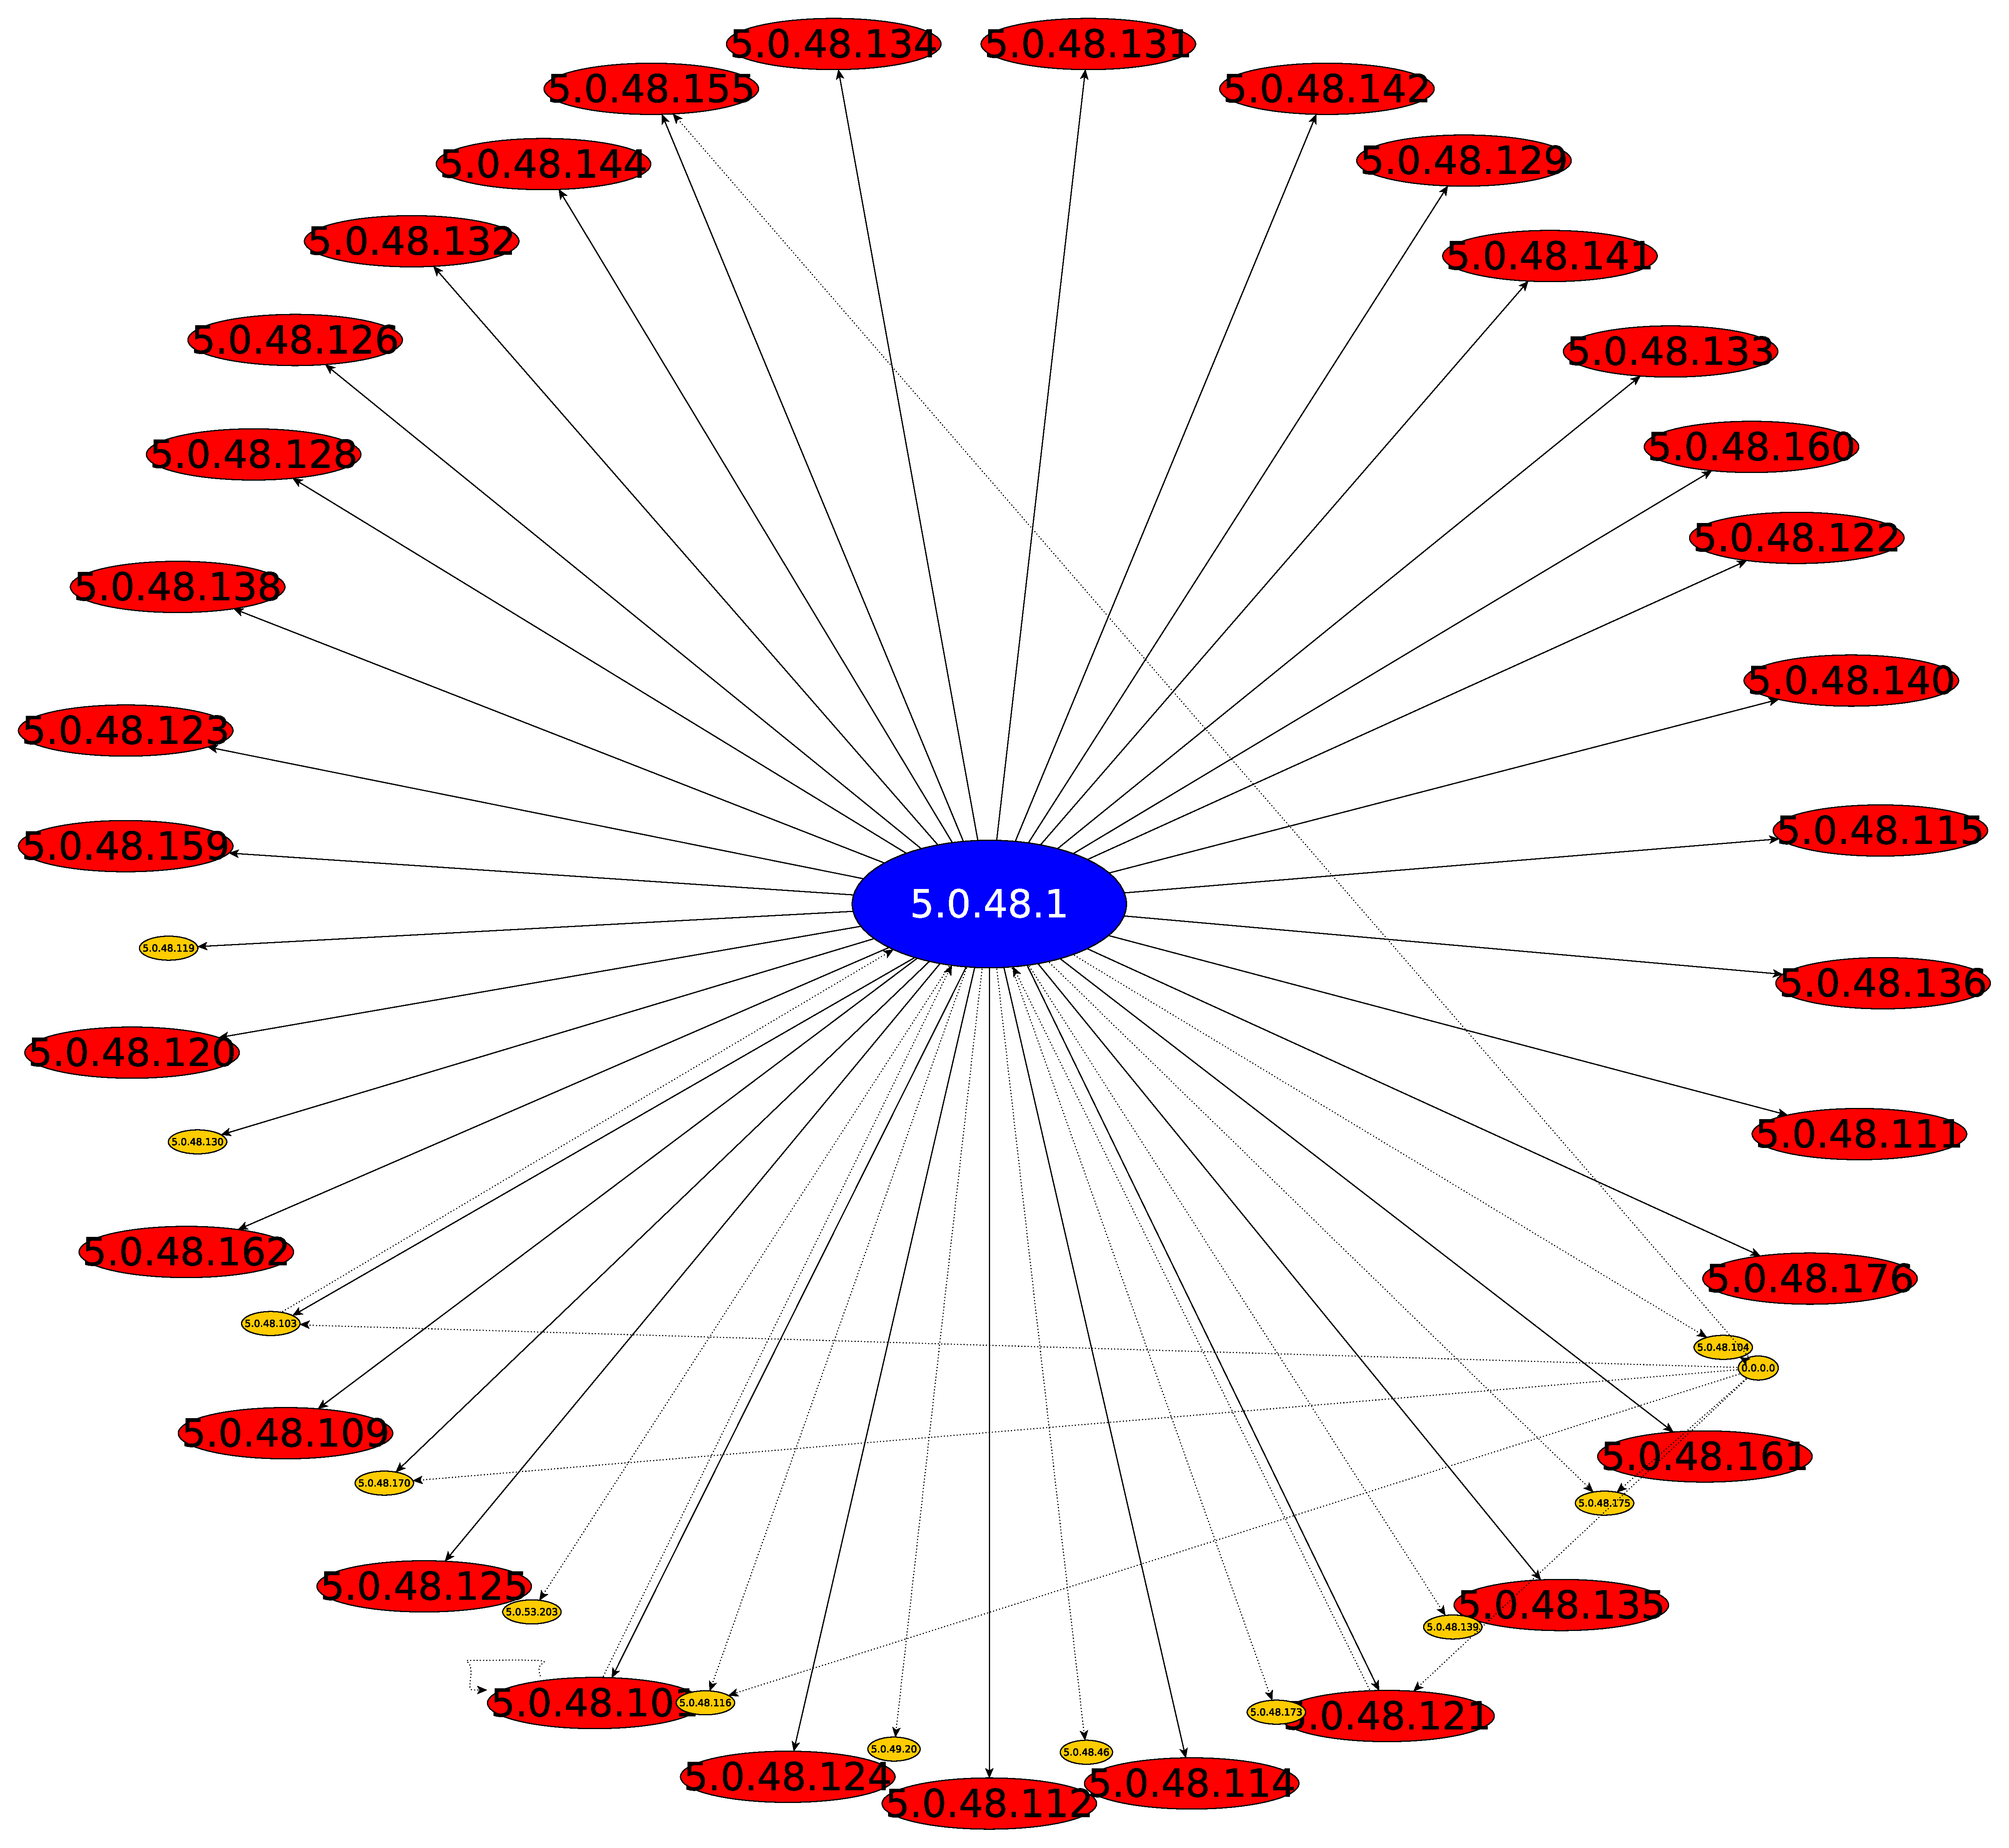
\includegraphics[width=0.5\textwidth]{img/graph/escenario_1/vlan40/vlan40}
    \caption{Grafo VLAN \nameref{itm:vlan40}}
    \label{fig:vlan40_grafo}
\end{figure}

\par Efectivamente se puede observar en el grafo que la red de tel\'efonia
IP parece trabajar con una topolog\'ia centralizada, al menos para cada vez
que deben resolver una \textit{MAC}, presumiblemente para realizar alguna
tarea que requiera de la utilizaci\'on de la red\footnote{Eso o la
telefon\'ia IP se utiliza muy poco en el datacenter.}.

\par As\'i pues, queda claro en la figura \ref{fig:vlan40_grafo} que nos encontramos
con un nodo principal que seguramente es la \textit{PBX} o servidor del
servicio de tel\'efon\'ia m\'ovil.


\subsubsection*{\underline{VLAN \nameref{itm:vlan40}: Conclusiones}}\label{subsubsec:vlan40_conclusiones}
\par Aqu\'i nos encontramos con una red que claramente se comporta distinta que el resto.
De la informaci\'on recolectada y los an\'alisis realizados, se pudo ver que
hay muy poco tr\'afico y por ende los valores de entrop\'ia y la cantidad
de IPs de la LAN nos permiten anticipar el comportamiento de la LAN sin
conocer detalles t\'ecnicos sobre la infraestructura o el software que 
utilizan los tel\'efonos.


    \subsubsection{VLAN de~\nameref{itm:vlan1}}


    %-------------------------------------------------------------------------------------

    %%\subsection{An\'alisis suplementarios}\label{sec:escenario1_supl}
\par Teniendo una gran cantidad de informaci\'on capturada en las distintas redes
que componen este escenario, corresponde quiz\'as hacer un an\'alisis un poco
m\'as profundo sobre las distintas variables que podemos identificar y guardar
durante la etapa de \textit{sniffing}.

\par Estas variables pueden ser muchas. En particular identificamos dos variables,
por ah\'i un tanto inmediatas y no muy complejas, pero no por ello menos importantes
o menos propensas a otorgarnos informaci\'on. Estamos hablando de la parametrizaci\'on
seg\'un el tiempo (cuando fue capturada cierta informaci\'on) y la cantidad (cuanta
informaci\'on).

\par As\'i pues, en un principio resulta interesante para comprender el comportamiento
de las redes ver el vol\'umen de paquetes ARP durante per\'iodos m\'as cortos. Hasta
este momento, en este escenario nos estuvimos concentrando en comprender a toda la
informaci\'on capturada como 2 grandes fuentes de informaci\'on (fuente origen y
fuente destino). Proponemos, entonces, observar que ocurre m\'as granularmente
al comprender a las fuentes de informaci\'on no como un \textit{todo}, sino analizando
que ocurr\'io cada d\'ia de captura.


\subsubsection{Vol\'umen de paquetes ARP por d\'ia/hora}
\par En la figura \ref{fig:arp_por_hora} se pueden observar como
va evolucionando la cantidad de paquetes capturados en per\'iodos de 60 minutos, y a
su vez comparar este comportamiento en los diferentes d\'ias.

\begin{figure*}[!b]
    \begin{tabular}{cc}
        \centering
        \subfloat[\nameref{itm:vlan10}]{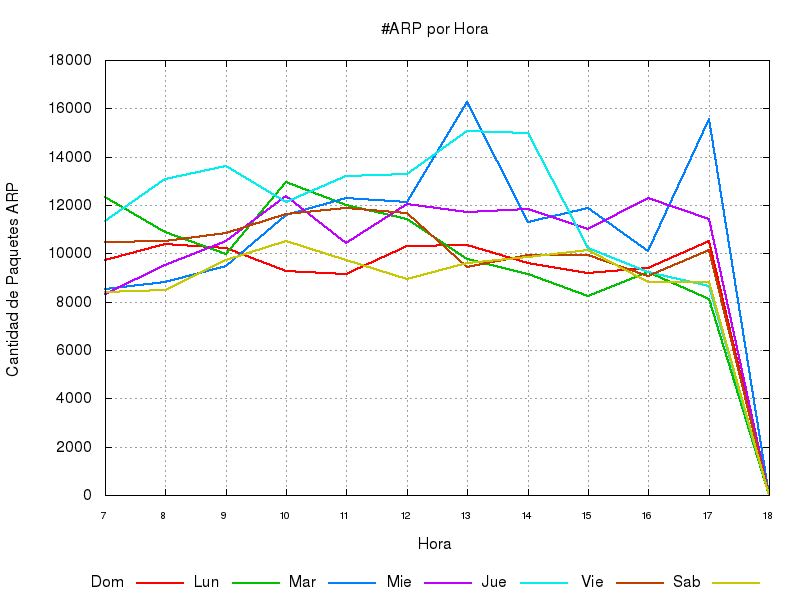
\includegraphics[width=0.5\textwidth]{img/graph/escenario_1/vlan10/vlan10_arp_per_hour_lines}} &
        \subfloat[\nameref{itm:vlan20}]{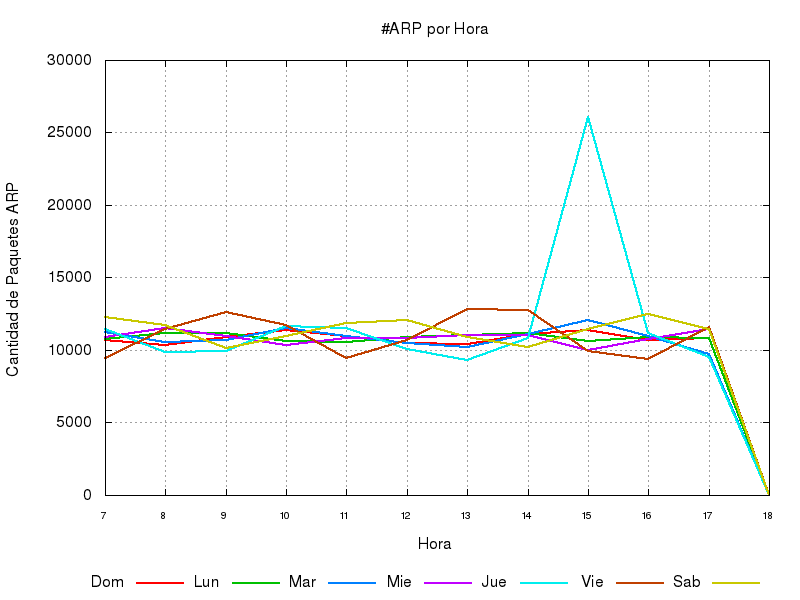
\includegraphics[width=0.5\textwidth]{img/graph/escenario_1/vlan20/vlan20_arp_per_hour_lines}} \\
        \subfloat[\nameref{itm:vlan40}]{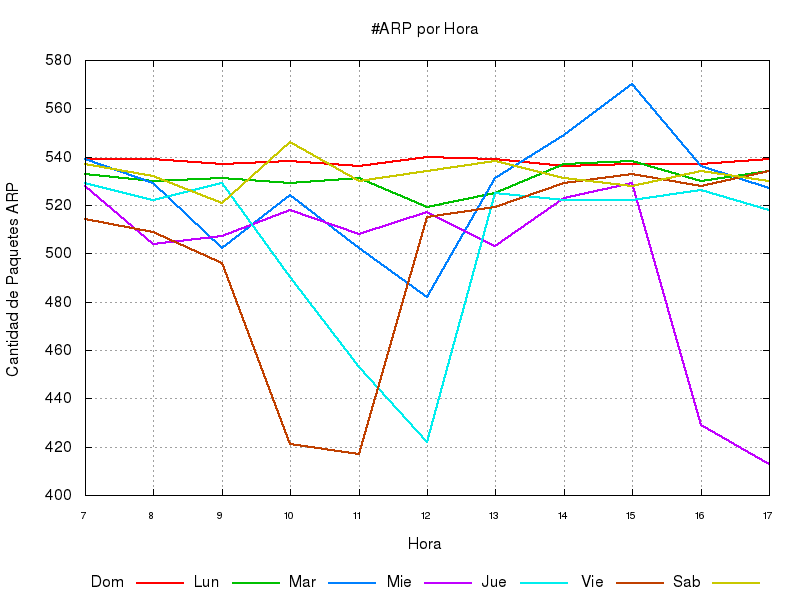
\includegraphics[width=0.5\textwidth]{img/graph/escenario_1/vlan40/vlan40_arp_per_hour_lines}} &
        \subfloat[\nameref{itm:vlan1}]{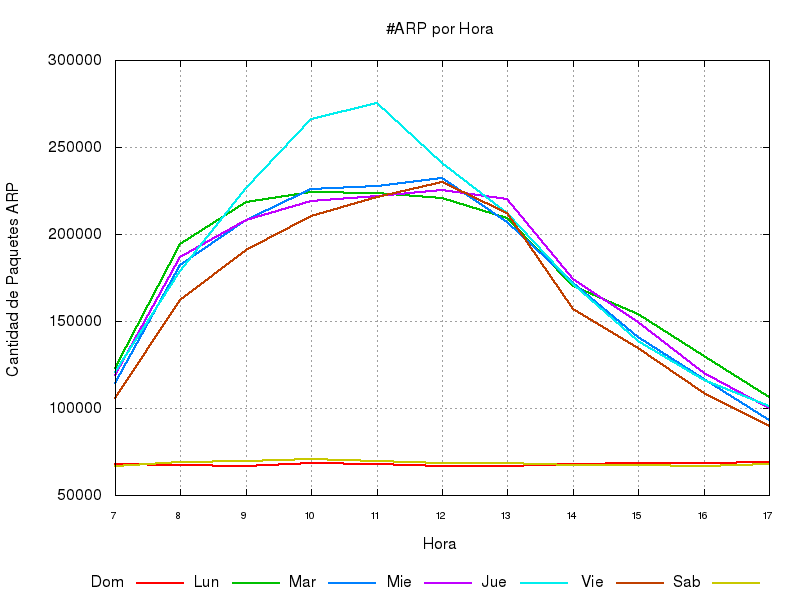
\includegraphics[width=0.5\textwidth]{img/graph/escenario_1/vlan1/vlan1_arp_per_hour_lines}} \\
    \end{tabular}
    \caption{Cantidad de paquetes ARP por hora}
    \label{fig:arp_por_hora}
\end{figure*}

\par Como primer resultado, que claramente salta a primera vista, es que el
comportamiento\footnote{Siempre pensado respecto de los paquetes ARP que se
encuentran en la red.} de las redes es bastante ca\'otico en cuanto a la cantidad
de paquetes por hora y d\'ia.

\par Claramente, el experimento realizado no nos permite decir exactamente que
est\'a ocurriendo en la red, pero si vemos que en el aspecto de como var\'ia
el vol\'umen de estos paquetes (y por lo tanto, una parte importante de la
congesti\'on de la LAN) nos encontramos con tres casos que parec\'ieran
seguir patron, mientras que la red de \nameref{itm:vlan40} pareciese,
\textit{a priori}, no hacerlo

\par Respecto de esto, y con el conocimiento que se tiene de que dispositivos/%
usuarios participan de la red, queda claro que el comportamiento aleatorio de
los usuarios con sus terminales (e incluso con terminales que un d\'ia est\'an
y otro no; o incluso que se conectan a la red en franjas horarias dispares)
tiene un impacto direct en la cantidad de paquetes que circulan en la red. M\'as
interesante, se puede observar que el vol\'umen es claramente m\'as alto en los
alrededores del mediod\'ia (comparando cada d\'ia en su variaci\'on por hora) y
en los d\'ias intermedios de la semana (comparando una misma hora pero en distintos
d\'ias)

\par Este \'ultimo detalle no s\'olo ocurre en la red de \nameref{itm:vlan10},
sino que tambi\'en se puede observar, y mucho m\'as marcado, en la red
\nameref{itm:vlan1}. Se observa aqu\'i que el vol\'umen es muy estable, bajo y
parejo los S\'abados y Domingos, y que durante los d\'ias de la semana se observa
un vol\'umen m\'as grande en la franja horaria de 9 a 14 hs, que luego se reduce
considerablemente hacia el fin de la jornada laboral\footnote{En particular, la
mayor\'ia de los usuarios de las redes observadas utiliza la red entre las 7 y
las 15 hs}. 

\par A pesar de ver este comportamiento similar, debemos aclarar
que los vol\'umenes de ambas redes son claramente distintos. Sin ir m\'as lejos,
en el caso promedio, la red \nameref{itm:vlan1} tiene 20 veces m\'as paquetes ARP
que \nameref{itm:vlan10}. Es decir, podr\'iamos tener una variacia\'on m\'as
grande, nominalmente hablando, dentro de esta red. Pero tomando en cuenta
el vol\'umen total y la cantidad de paquetes, es admitible la comparaci\'on.

\par Algo remarcable de esta similitud reci\'en expuesta, es que la red de
\nameref{itm:vlan1} tiene muchos servidores aparte de usuarios, y si obsevamos
el grafico correspondiente a la red \nameref{itm:vlan20}, veremos un vol\'umen
similar al de la red \nameref{itm:vlan10} y de comportamiento igualmente
dispar\footnote{M\'as all\'a del \textit{outlier} correspondiente a las
15 hs del Jueves. Probablemente hubo alguna instalaci\'on de servidores o
software en los mismos que impactaron en la red.}. Al observar
una red que combina, esperablemente, los comportamientos de estos dos tipos
de redes, nos encontramos con una red que tiene un vol\'umen base seguramente
dependiente de los servidores\footnote{ya que estos no suelen desconectarse y
tienen un comportamiento m\'as estable que las terminales de usuarios}
(claramente observable en las l\'ineas que corresponde nal S\'abado y Domingo)
y luego durante los d\'ias de semana con la afluencia de las terminales de
los empleados, se ve como el vol\'umen se incrementa not\'ablemente.

\par En cuanto a la red de \nameref{itm:vlan40}, simplemente podemos ver
que maneja un vol\'umen que no pareciese seguir un patr\'on respecto
de las horas ni los d\'ias. No s\'olo eso, sino que el vol\'umen que manejan
pareciera ser m\'as estable que en el resto de los casos (mucha menos
variaci\'on de vol\'umen por hora y d\'ia). As\'i pues, podemos determinar
que estos dispositivos (al menos los que se utilizan en esta red, no podr\'iamos
hacer la siguiente aserci\'on para todas las redes de telefon\'ia) hacen un
uso distinguiblemente menor en cuanto a la identificaci\'on de las \textit{MAC}
de los dem\'as. Esto tambi\'en podr\'ia deberse a que la cantidad de dispositivos
conectados es mucho menor y por ah\'i los dispositivos tienen suficiente
espacio en su tabla ARP para no requer\'i consultar a la red tan seguido por la
resoluci\'on de una IP.


\subsubsection{Relaci\'on entrop\'ia - vol\'umen diario de paquetes ARP}
\begin{figure*}[!ht]
    \begin{tabular}{cc}
        \centering
        \subfloat[\nameref{itm:vlan10}]{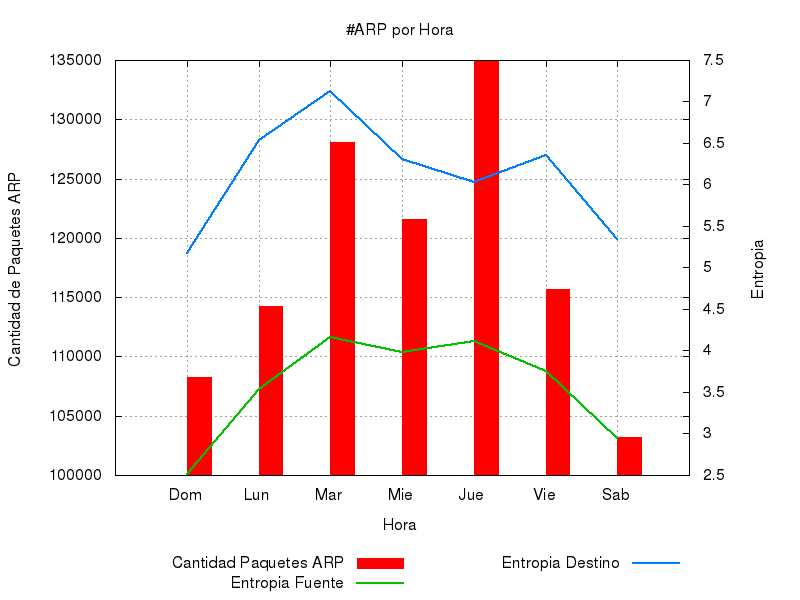
\includegraphics[width=0.5\textwidth]{img/graph/escenario_1/vlan10/vlan10_arp_vs_entropia}} &
        \subfloat[\nameref{itm:vlan20}]{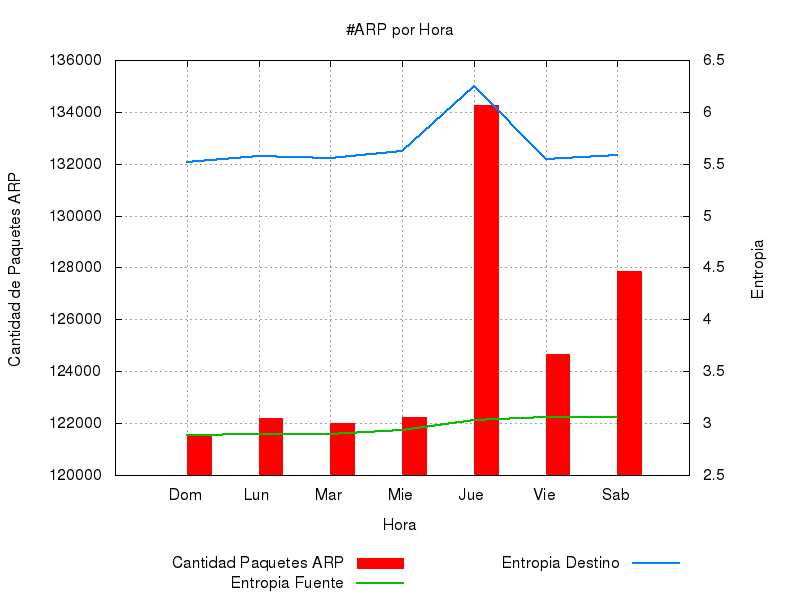
\includegraphics[width=0.5\textwidth]{img/graph/escenario_1/vlan20/vlan20_arp_vs_entropia}} \\
        \subfloat[\nameref{itm:vlan40}]{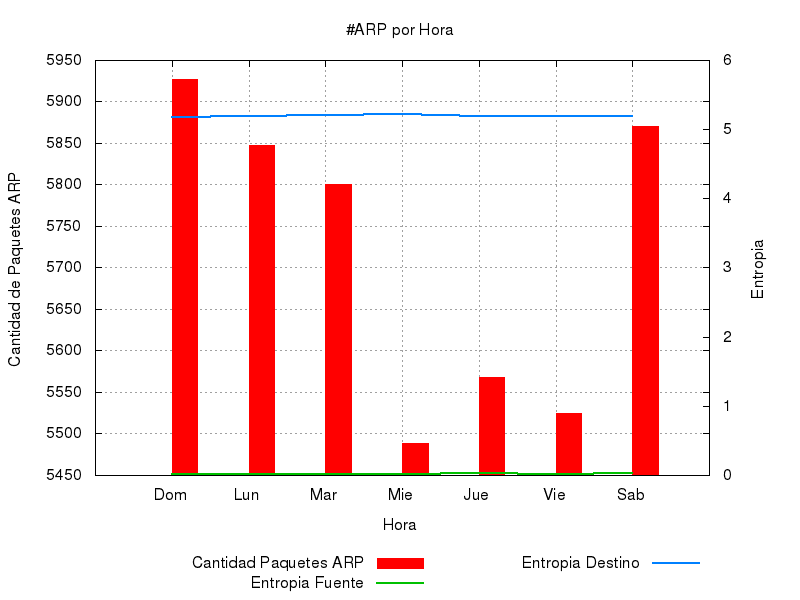
\includegraphics[width=0.5\textwidth]{img/graph/escenario_1/vlan40/vlan40_arp_vs_entropia}} &
        \subfloat[\nameref{itm:vlan1}]{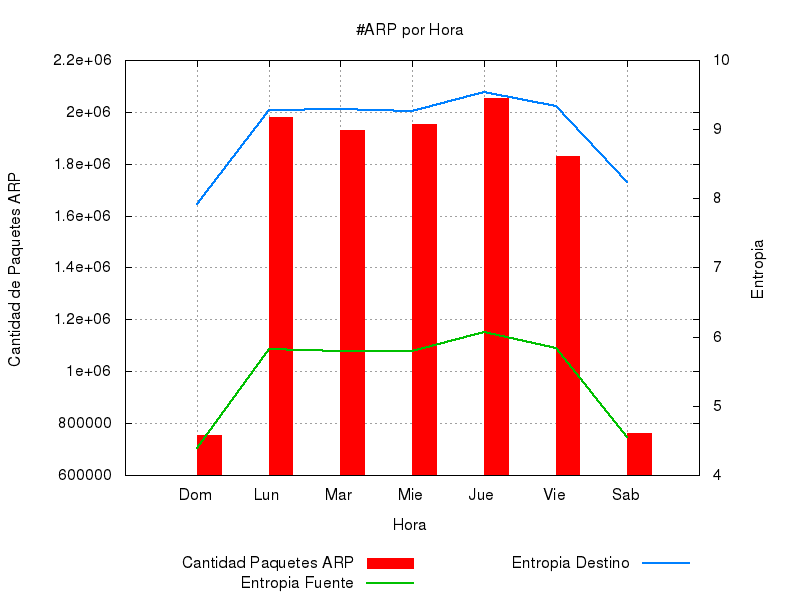
\includegraphics[width=0.5\textwidth]{img/graph/escenario_1/vlan1/vlan1_arp_vs_entropia}} \\
    \end{tabular}
    \caption{Cantidad de paquetes ARP por hora}
\end{figure*}


    %\subsection{Conclusiones Preliminares}



\section{Escenario 2}
	\IEEEPARstart{E}{N} este segundo escenario, la universidad elegida fue la Universidad de Helsinki\cite{helsinki}, ubicada en \emph{Helsinki, Finlandia}. 

\par Para este experimento, realizamos 500 pedidos al host de la p\'agina web del Departamento de Computaci\'on de dicha universidad\cite{helsinkics}. 

\subsection{Resultados para el total de los Experimentos}
\par Igual que en el escenario anterior, primero vamos a determinar cuantas veces apareci\'o cada secuencia de nodos:

\begin{table}[h]
    \centering
    \begin{tabular}{c | c}
                   &\#Caminos \\
      \#Aparicione &Distintos \\
      \hline\hline
       	1& 51\\
       	2& 9\\
        3& 5\\
        4& 5\\
		5& 2\\
        6& 2\\
        7& 2\\
        8& 2\\
        9& 1\\
       10& 1\\
       26& 2\\
       28& 1\\
       31& 1\\
       80& 1\\
      134& 1\\       
      \hline\hline
    \end{tabular}
    \bigskip
    \caption{Frecuencia por \emph{path} de hops obtenida}
    \label{tab:helsinki_sec_hops}
\end{table}

\par A diferencia del escenario anterior, nos encontramos con mucha mayor variabilidad en las rutas. A pesar de tener un claro ganador, las tres rutas con mayor cantidad de apariciones no llegan a acumular ni un 50\% del total de la experimentaci\'on.

\par Procedemos entonces a realizar el an\'alisis sobre la ruta con 134 apariciones. En la figura \ref{fig:rtt_dev_helsinki} podemos observar la media de RTT para cada TTL, junto con su desv\'io estandar y todas sus mediciones.

\begin{figure}
    \centering
    %\includegraphics[width=0.5\textwidth
    %                ]{img/escenario2/{hel_134.path.86.rtt_acum}.pdf}
    \caption{RTT media/Desv\'io Est\'andard}
    \label{fig:rtt_dev_helsinki}
\end{figure}

\par En este caso, lo primero que notamos es una anomalía en el salto 2, en el que se ve que el desv\'io estandar es muy grande (y teniendo mediciones de RTT que se acercan a 1 segundo). Si no tenemos en cuenta este hop, el resto de los resultados parecen bastante aceptables, aunque se repite el comportamiento de tener hops continuados con RTT similares y peque\~nas oscilaciones.

\par Procedemos entonces a filtrar los datos de manera similar al caso anterior, para quedarnos con los nodos que nos aporten información, y no perjudiquen el cálculo del $ZScore$. En la figura \ref{fig:rtt_dev_helsinki_filtered} se observa como nos quedan los datos luego del proceso.

\begin{figure}
    \centering
    %\includegraphics[width=0.5\textwidth
    %                ]{img/escenario2/{hel_134.path.86.rtt_acum_filtered}.pdf}
    \caption{RTT media/Desv\'io Est\'andard para Hops Relevantes}
    \label{fig:rtt_dev_helsinki_filtered}
\end{figure}

\par Con esta informaci\'on filtrada, pasamos a calcular el $ZScore$ para cada hop. El resultado se ve en la figura \ref{fig:zscore_helsinki_filtered}

\begin{figure}
    \centering
    %\includegraphics[width=0.5\textwidth
     %               ]{img/escenario1/{hel_134.path.86.rtti_salteando_zscore_filtered}.pdf}
    \caption{$ZScore$ por $RTT_i$}
    \label{fig:zscore_helsinki_filtered}
\end{figure}


\section{Escenario 3}
	\subsection{Descripci\'on del Escenario}
	\par En este escenario se monitorearon los paquetes ARP de la red Wi-Fi de acceso público de un local de comida rápida en una zona muy concurrida de la ciudad de Buenos Aires, un Starbucks en Av. Callao.

	\par A la hora del análisis, se desconoce la naturaleza de la red, quienes intervienen en la misma y el accionar de los usuarios en ella.
    
    \par Se espera que en general las conexiones de los diversos dispositivos de quienes se encuentran en el local sea de algunos pocos minutos y busque simplemente acceder a internet, por lo cual se espera que la principal conmutación se de entre las IPs de estos dispositivos y el \emph{gateway}.


\subsection{An\'alisis de datos obtenidos}
	\par La captura fue de 45 minutos y se enviaron 947 paquetes, el grafo dirigido de conexiones que se obtuvo fue el siguiente:

 %[-Grafo-]
 
\begin{figure}[H]
		\centering
		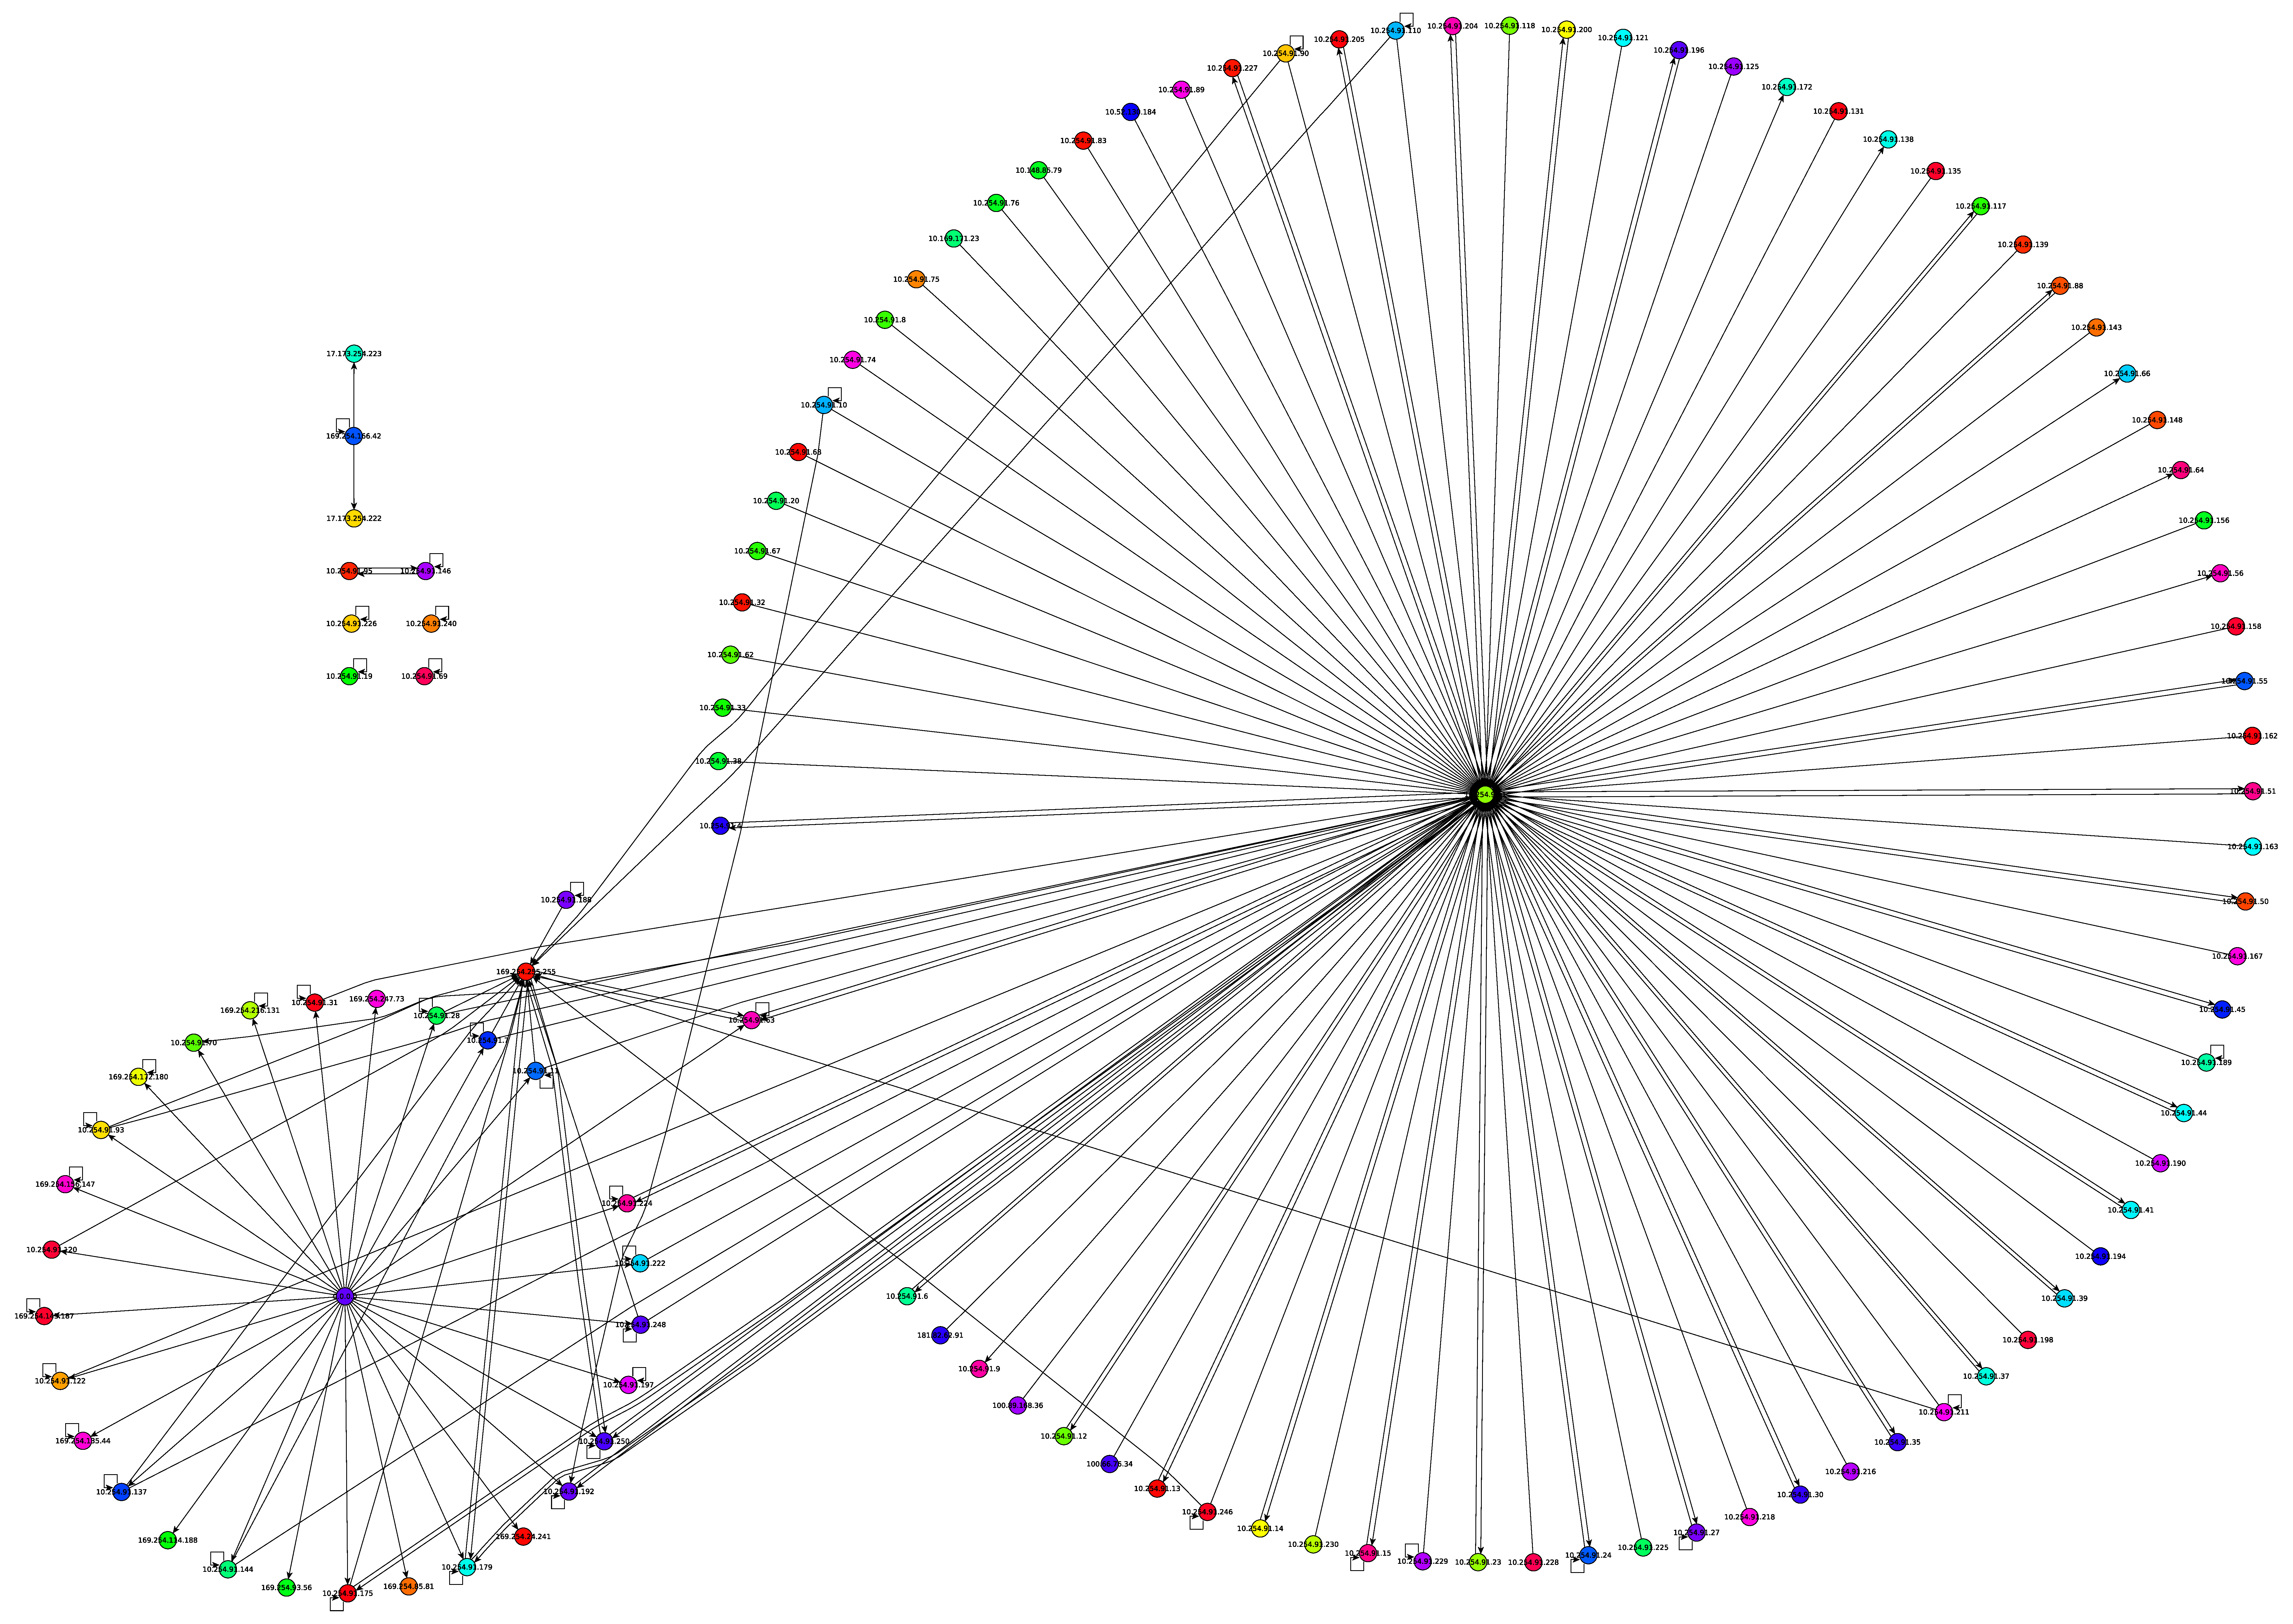
\includegraphics[width=0.5\textwidth]{img/graph/escenario_3/starbucks2.eps}
		\caption{Grafo de la red del Escenario 3}
		\label{fig:grafo_escenario3}
	\end{figure}

		\par Como el grafo es de gran tamaño vamos a considerar subgrafos donde se encuentran nodos interesantes para el análisis.

	\par Hay dos direcciones involucradas en gran parte del tráfico de paquetes, 10.254.91.1 que  recibe y envia hacia una gran cantidad de IPs y 169.254.255.255 que principalmente es destino.

	\par La primera se comporta como el gateaway, interactua con la mayoria de las IPs y es la más activa de toda la red.   Como se ve ampliando la figura 1, la cantidad de direcciones que le envian paqueteses increiblemente grande.

%[-Zoom a IP 10.254.91.1-]

\begin{figure}[H]
		\centering
		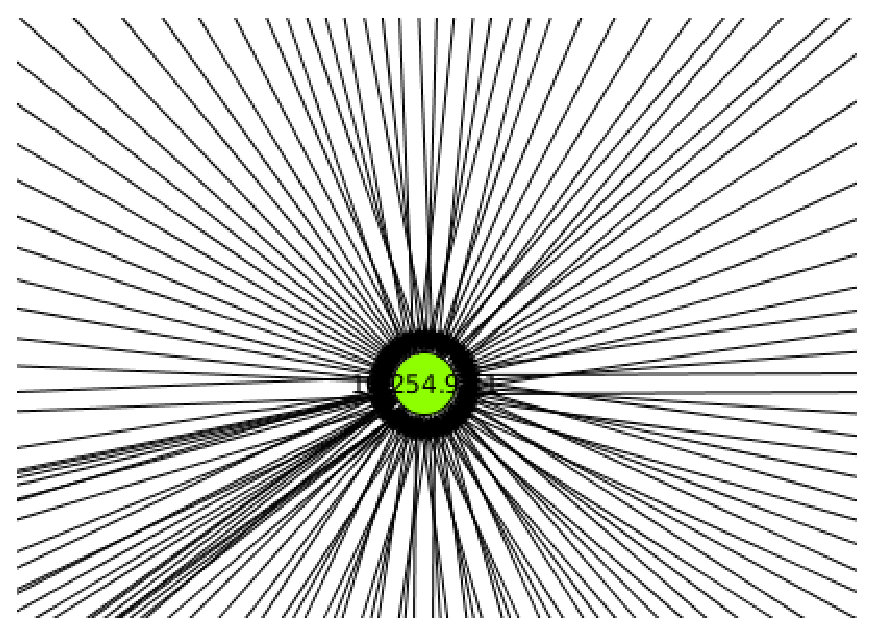
\includegraphics[width=0.5\textwidth]{img/graph/escenario_3/10254.eps}
		\caption{Ampliación en la cercan\'ia a 10.254.91.1}
		\label{fig:gateway_escenario3}
\end{figure}
	\par Tras investigar un poco al respecto, encontramos que la segunda IP mencionada es una dirección reservada  a la que los dispositivos envian paquetes ARP al no encontrar el servidor DHCP ya sea por recien conectarse o perder la ruta hacia el , el dispositivo se asigna una direccion para acceder y comunicarse a la red que usará hasta que se le asigne una IP mediante DHCP. \footnote{http://www.ietf.org/rfc/rfc3927.txt}
	\par Si nos quedamos solamente con aquellos hosts que interactúan con 169.254.255.255 se obtiene el siguiente grafo:   

%[-Vecindad de la IP 169.254.255.255-]
\begin{figure}[H]
		\centering
		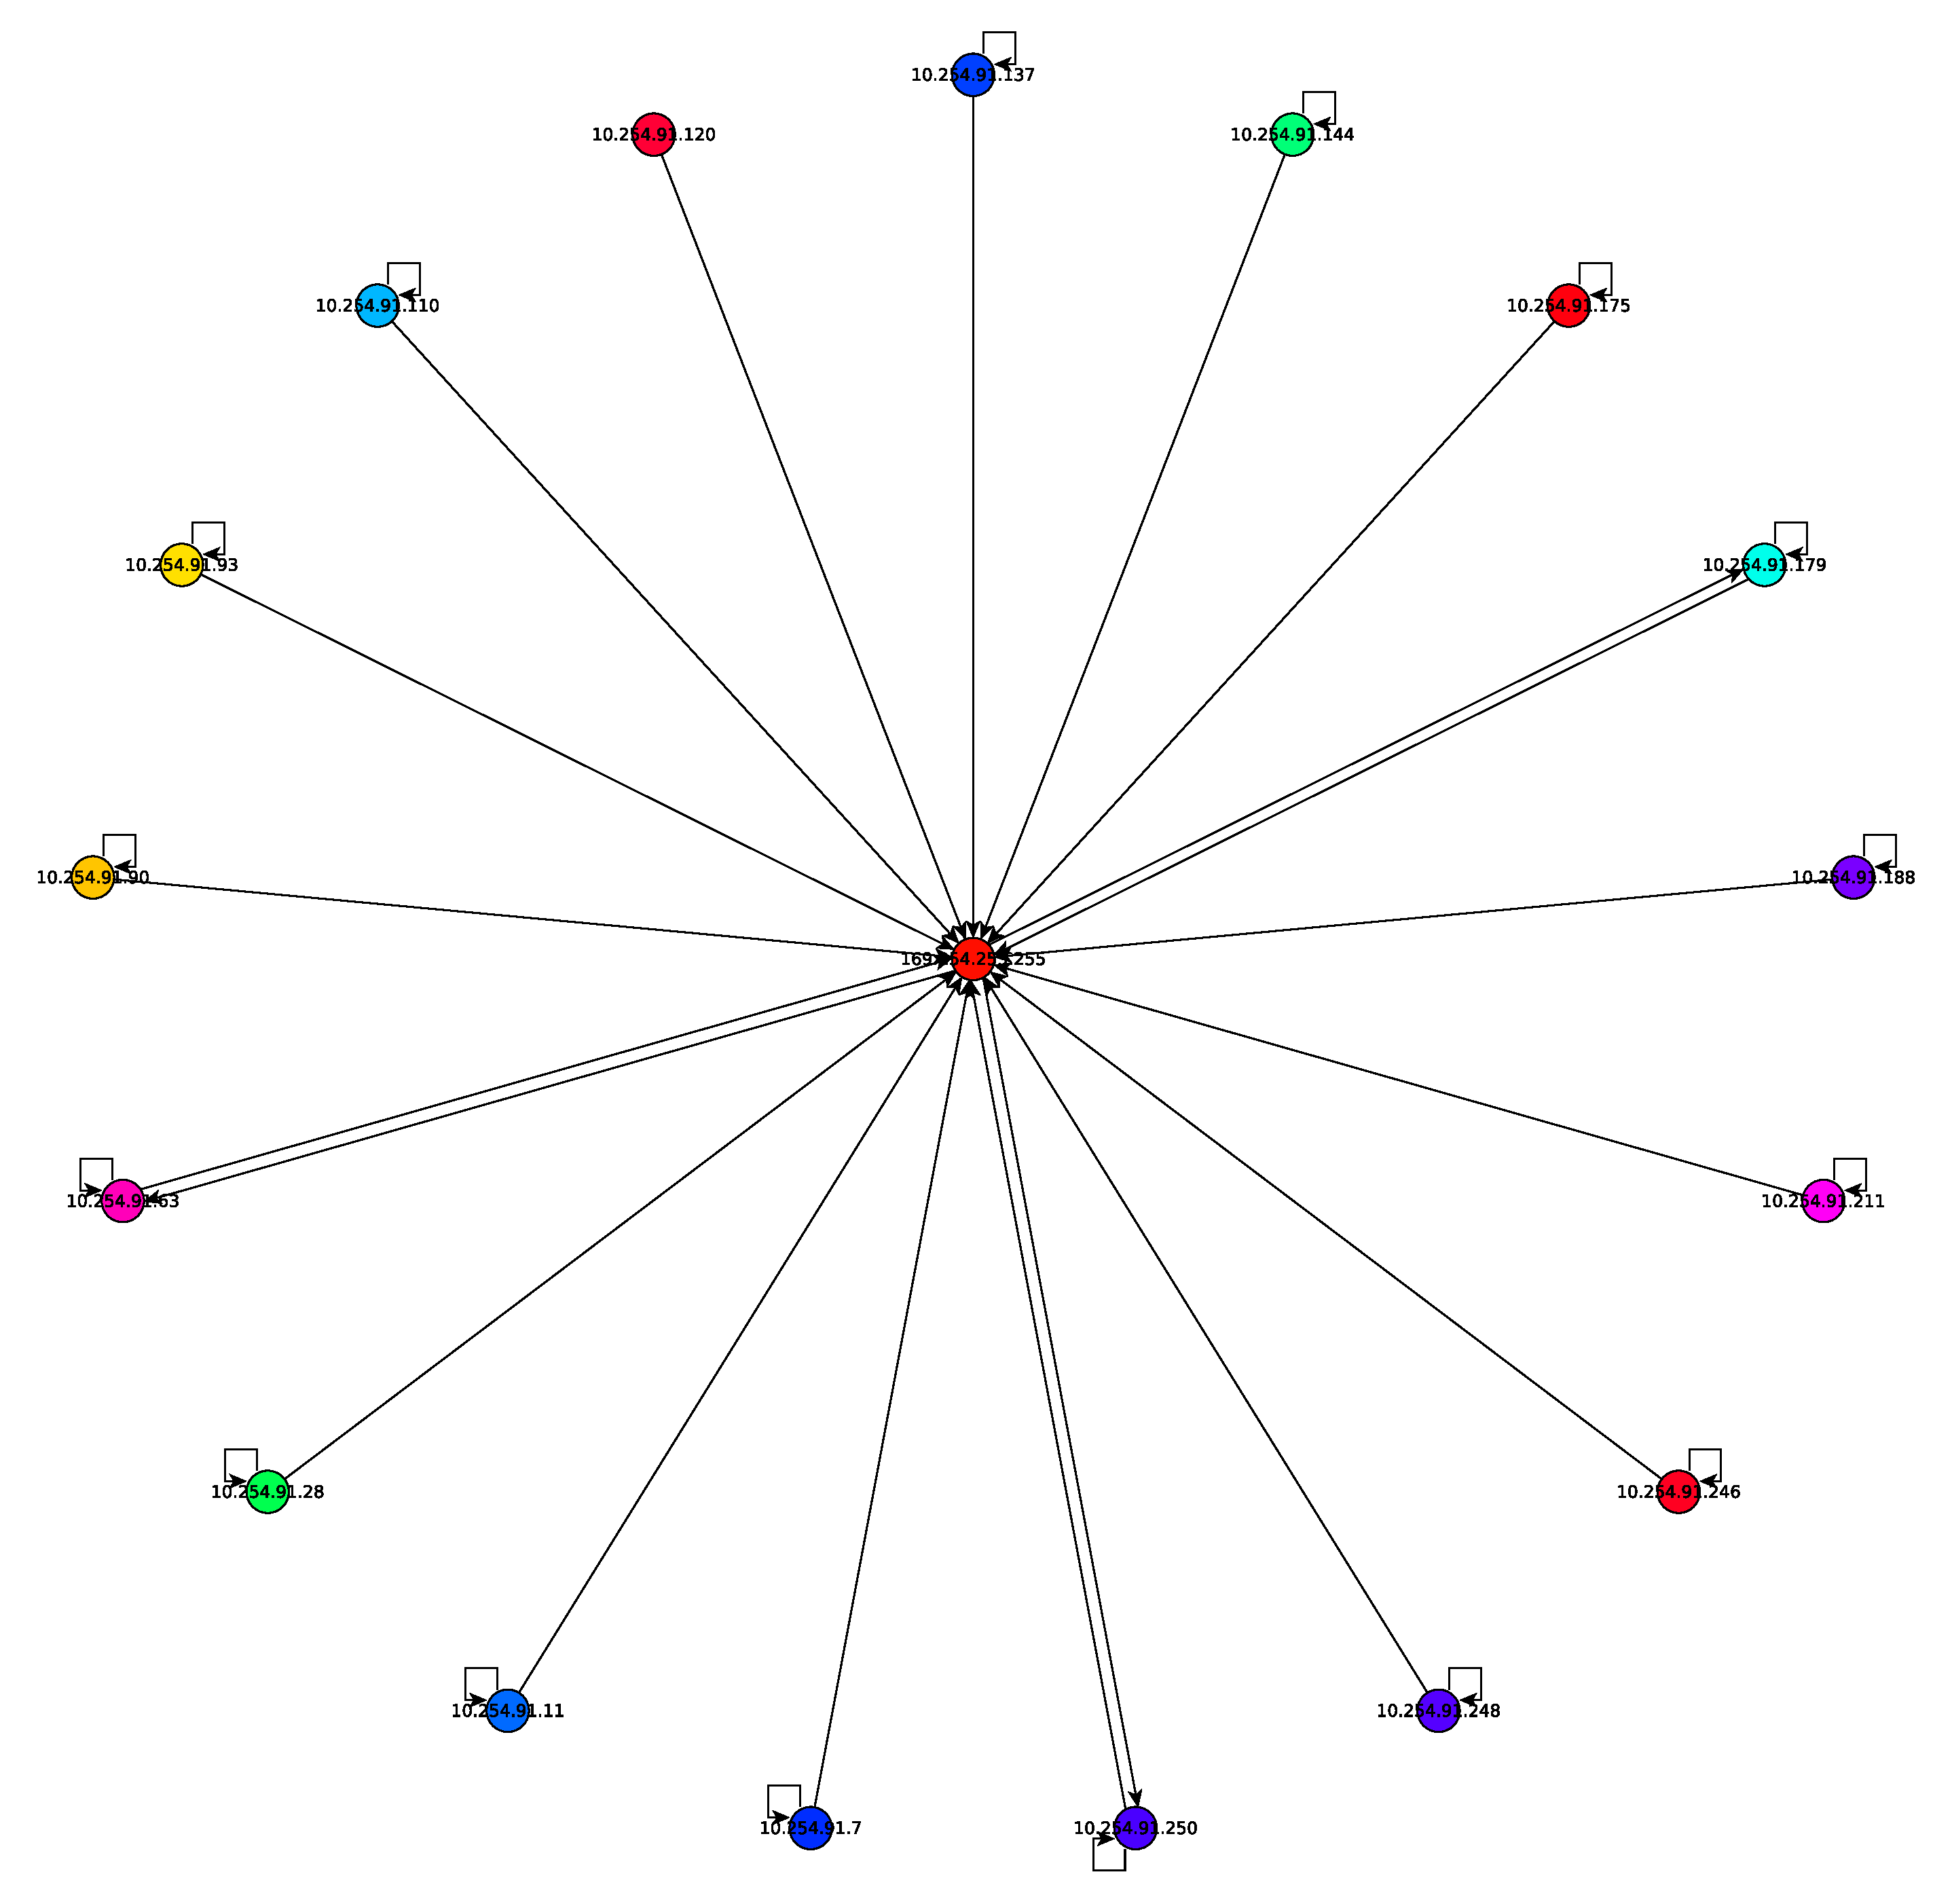
\includegraphics[width=0.5\textwidth]{img/graph/escenario_3/169254_aislado.eps}
		\caption{Vecindad de la IP 169.254.255.255}
		\label{fig:v1_escenario3}
\end{figure}
	\par Tambien se destaca que hay varios paquetes con origen 0.0.0.0, esto se da porque  al conectarse a la red ciertos dispositivos  envian broadcast para ser detectados por el servidor DHCP y que se les asigne una IP, luego terminan recibiendo paquete ARP con la IP asignada.
    
    \par De la misma forma que hicimos antes, se puede generar el grafo de la vecindad a 0.0.0.0 y resulta similar al presentado anteriormente.
    
%[-Vecindad de la IP 0.0.0.0-]
\begin{figure}[H]
		\centering
		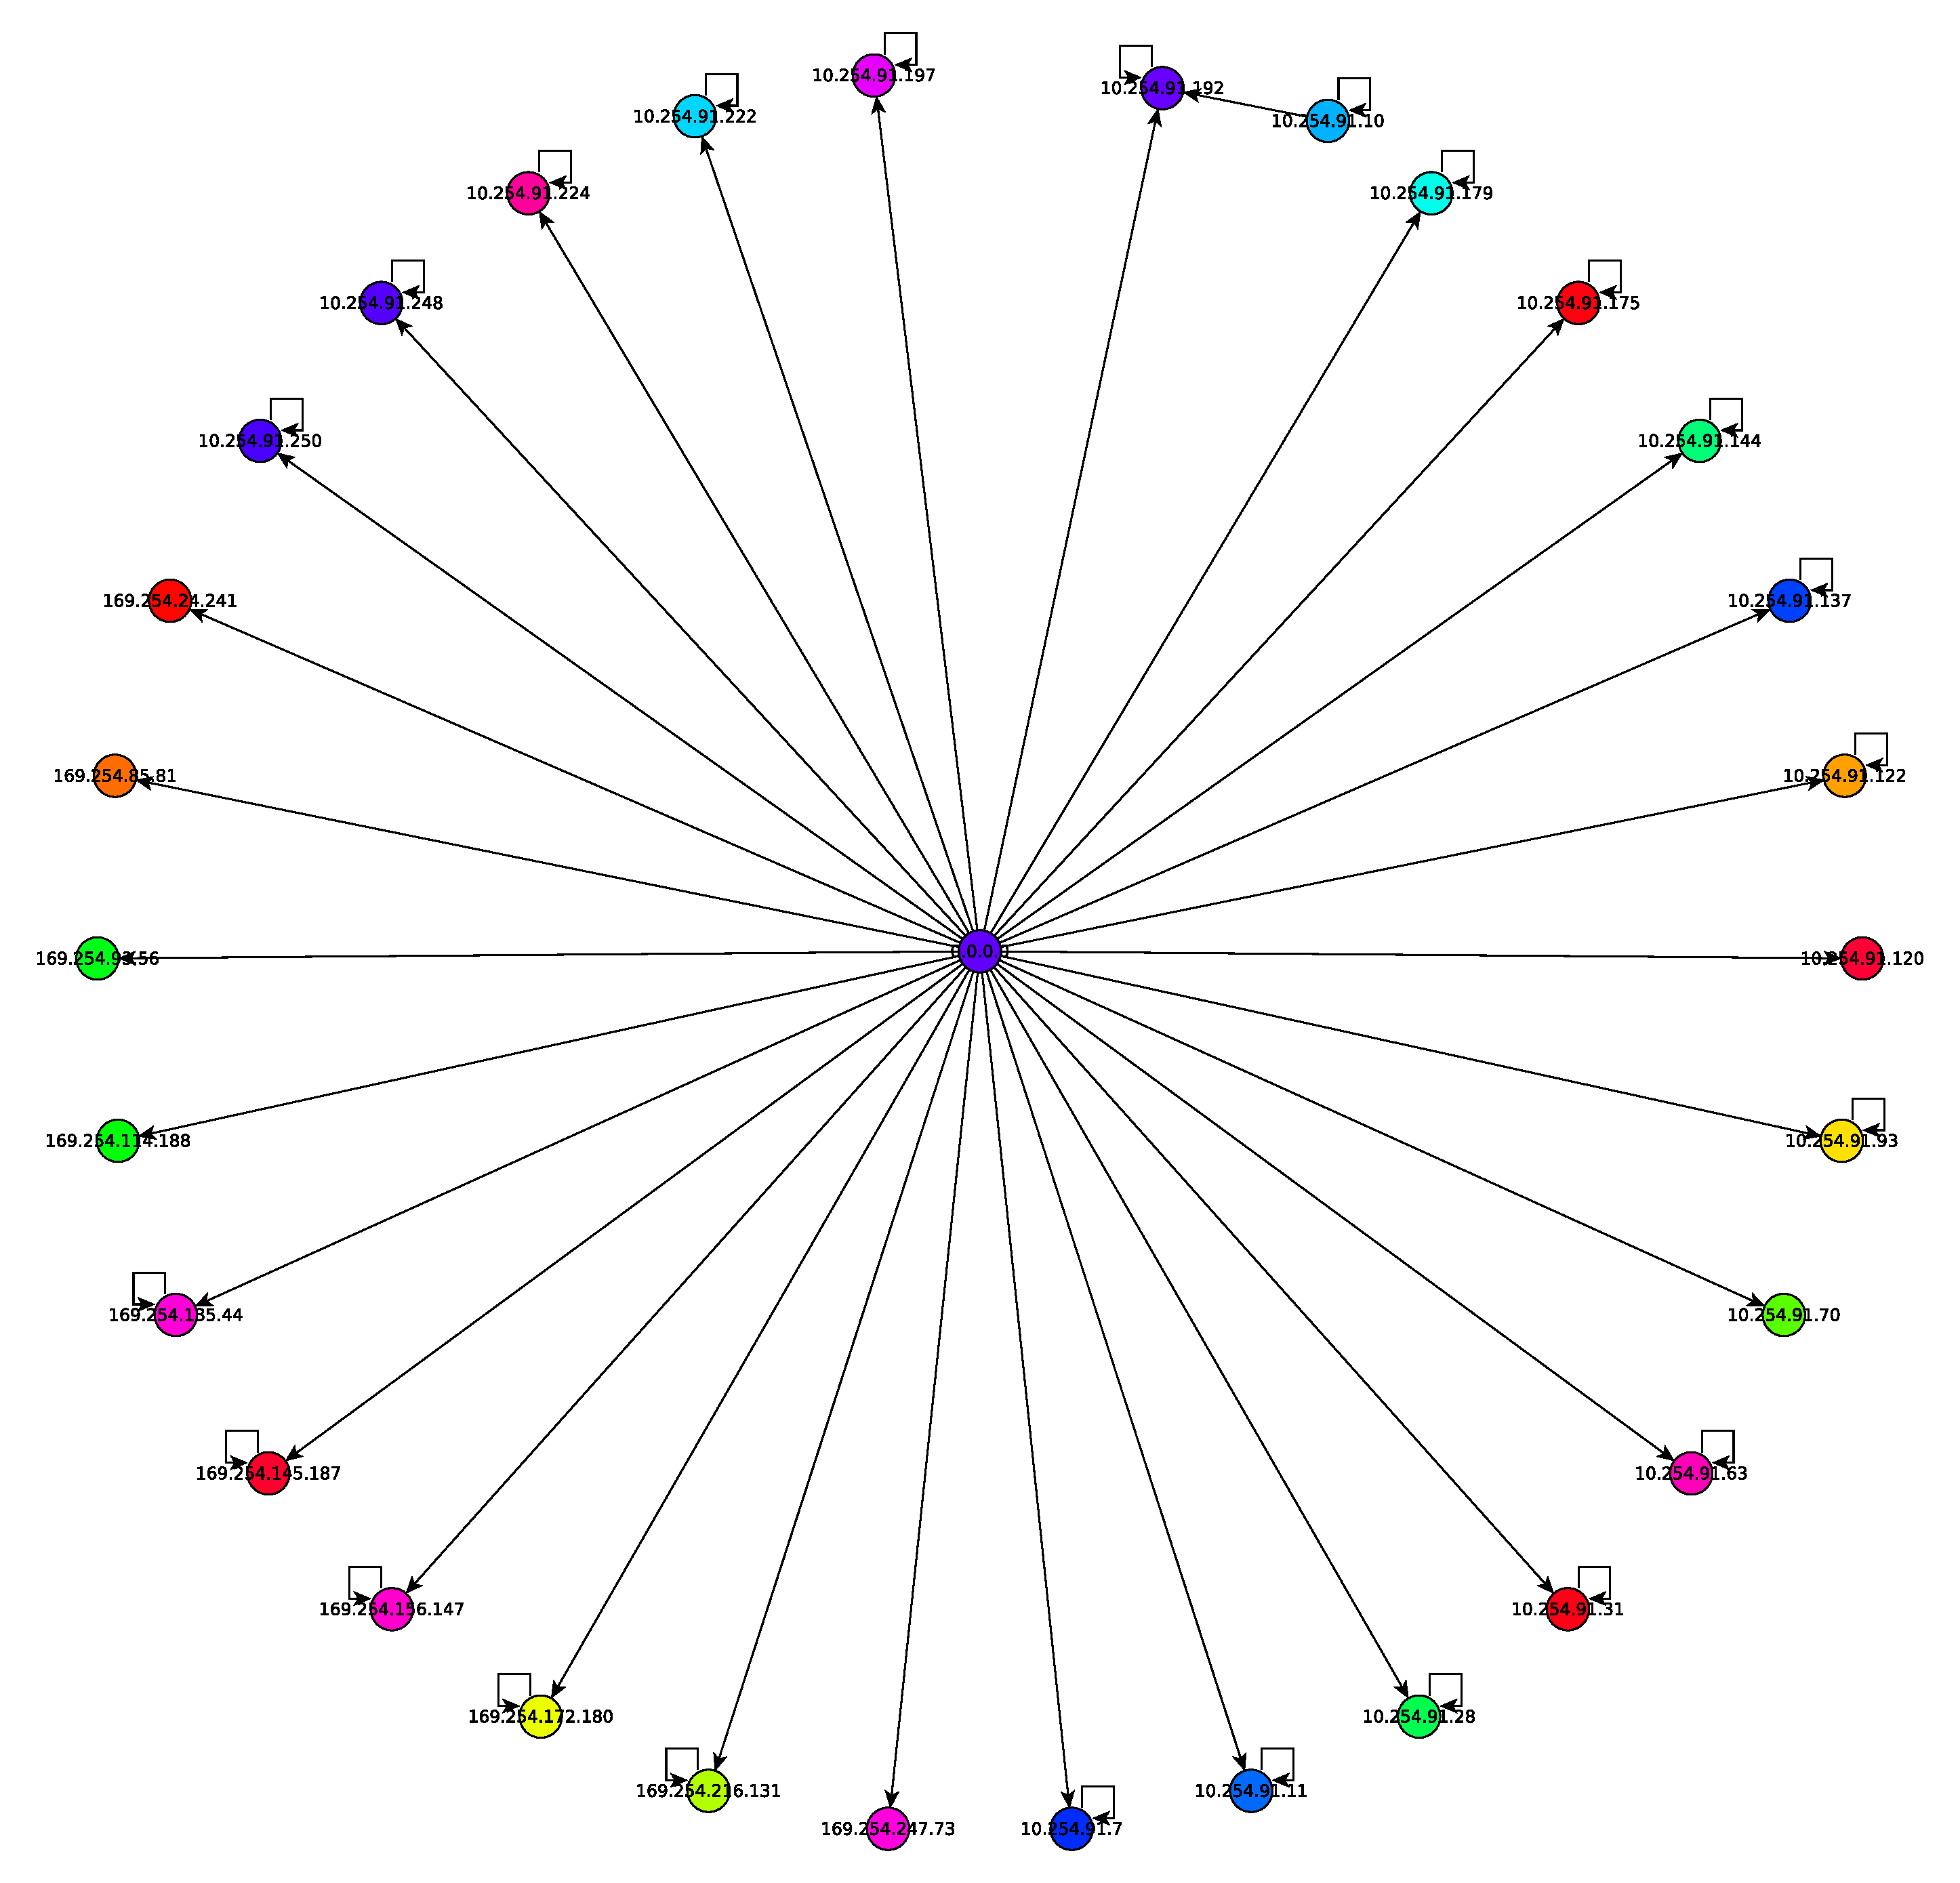
\includegraphics[width=0.5\textwidth]{img/graph/escenario_3/0000_aislado.eps}
		\caption{Vecindad de la IP 0.0.0.0}
		\label{fig:0_escenario3}
\end{figure}

	\par Al solo restringirnos a estos nodos, podemos ver que varios hosts que se encontraban en esta situación.
\vspace{6 mm}

	\par El resto de las direcciones se encuentran en el rango 10.254.0.0/16, lo cual es completamente razonable y 169.254.0.0/16 que es un caso más interesante, estas direcciones son conocidas como \emph{Link-local addresses}, son direcciones reservadas asignadas en Windows cuando no se puede establecer contacto con el servidor DHCP y se genera su propia IP mediante el direccionamiento conocido como APIPA. \footnote{http://wiki.wireshark.org/APIPA}

	\par El sistema operativo intentará constantemente conectarse con DHCP y recibir una IP válida, mientras tanto los hosts con estas direcciones pueden comunicarse entre sí dentro de la red, pero no con ninguno externo a la red local.
\vspace{6 mm}
	\par Algunas otras caracteristicas del grafo son:

\begin{itemize}

\item Nodos Aislados:

\par En el grafo se presentan nodos que podemos definir como aislados dado que no se comunicaron con el gateway y no son conexos  al resto del grafo.
    
\par Estos dispositivos se comunican entre sí, con si mismos, o con nadie como es el caso de 17.173.254.223 que no envia paquetes.

\par  Como es minimamente necesario que envien un paquete a 10.254.91.1 luego de ingresar a la red, nos hace suponer que el host se encontraba conectado a la red antes de hacer el análisis y de esta forma obtuvieron su direccion.  
\end{itemize}

%[-Subgrafo con nodos aislados-]
\begin{figure}[H]
		\centering
		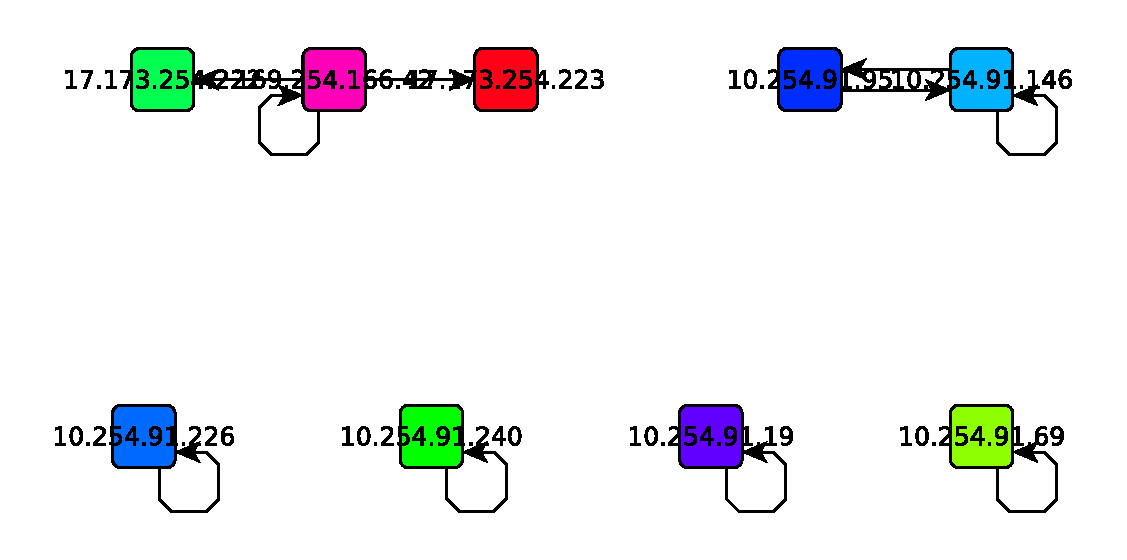
\includegraphics[width=0.5\textwidth]{img/graph/escenario_3/nodos_aislados.eps}
		\caption{Nodos considerados como aislados}
		\label{fig:aislados_escenario3}
\end{figure}


\begin{itemize}
\item Nodos Reflexivos:
\par Podemos notar que algunos nodos envían paquetes a si mismos, algunos motivos por los que puede suceder esto es para actualizar la tabla ARP, para buscar duplicados de la direccion IP o cambios de la direccion MAC. Este envío de paquetes se conoce como Gratuitous ARP.  \footnote{http://wiki.wireshark.org/Gratuitous\_ARP}
\end{itemize}

\subsubsection{Informaci\'on y Entrop\'ia}
		        
	\par En cuanto al análisis de la información de cada simbolo de ambas fuentes, primero calculamos la probabilidad muestral de ambas fuentes.
	\par Las siguientes tablas muestran las 5 IPs con mayor probabilidad muestral obtenidas, tanto para la fuente $S_{src}$ como para $S_{dst}$, decidimos mostrar solo cinco en el orden decreciente ya que a partir de las siguientes la diferencia es menor a 0.005 y se hace imposible apreciarlo en los graficos.

\newpage

\begin{figure}[!ht]
    \centering
    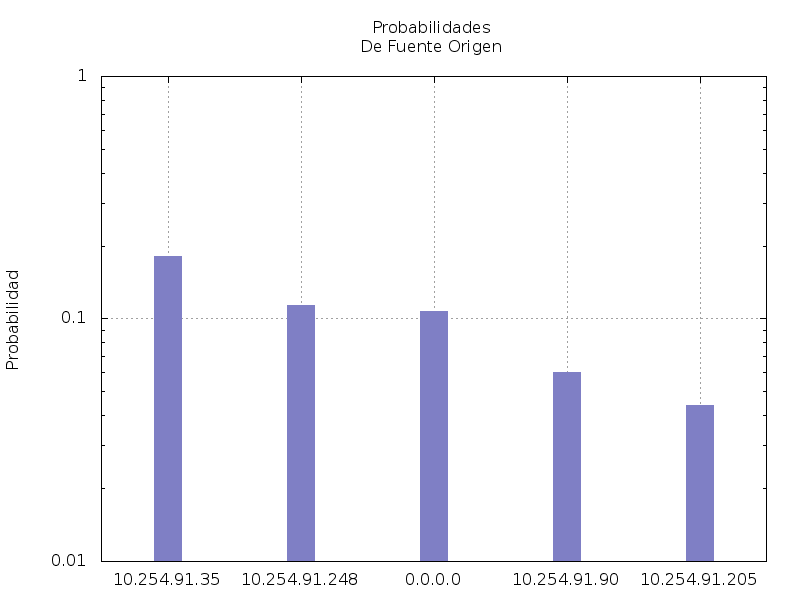
\includegraphics[width=0.5\textwidth]{img/graph/escenario_3/proba_src.png}
\end{figure}


\begin{figure}[!ht]
    \centering
    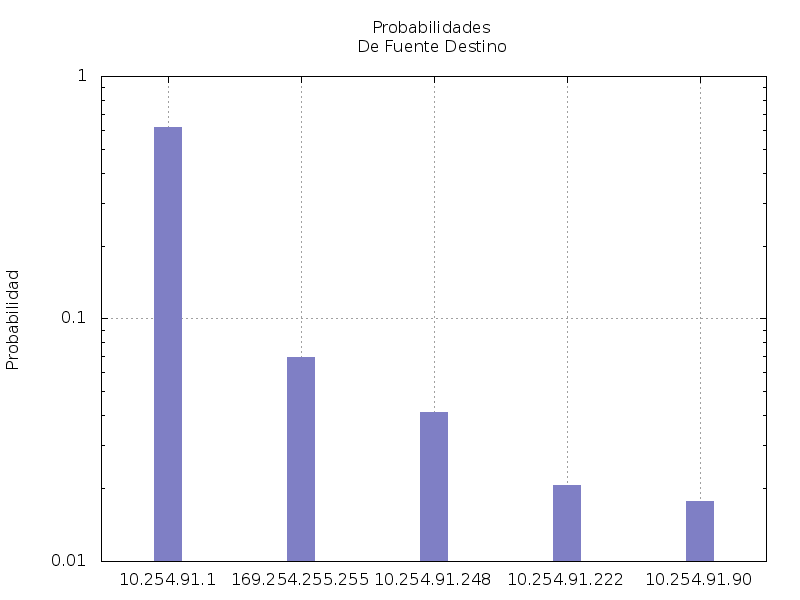
\includegraphics[width=0.5\textwidth]{img/graph/escenario_3/proba_dst.png}
\end{figure}


	\par Para los paquetes de destino, los resultados se corresponden con lo visto al hacer el grafo tanto en los valores de probabilidad como en la proporcionalidad con las demas direcciones, 10.254.91.1 tiene una probabilidad tan alta, que hace necesario mostrar el grafico en escala logaritmica para poder apreciar los valores del resto de las probabilidades. Algo similar a lo que sucede con el grafo, donde la mayoría de los paquetes eran enviados a dicha dirección.
	\vspace{6 mm}

	\par En el caso de la fuente destino, no encontramos ningun comportamiento visto anteriormente, los valores nos muestran que todas las direcciones se acercaron a la media general de envíos de paquetes, inclusive la direccion 0.0.0.0, que al ver el grafo imaginamos que era quien más envios habia realizado. 


	\par A partir de estos valores podemos ver el nivel de información que nos da cada una de estas IPs.

	\par Como ya sabemos la información de cada simbolo $p_{i}$ se obtiene al calcular:

\begin{equation}
	\log_2 (\frac{1}{ p_{i} })
\end{equation}

	\par Al ser una función decreciente, aquellas direcciones del grafico anterior con mayor probabilidad son las de menor información:

\begin{figure}[!ht]
    \centering
    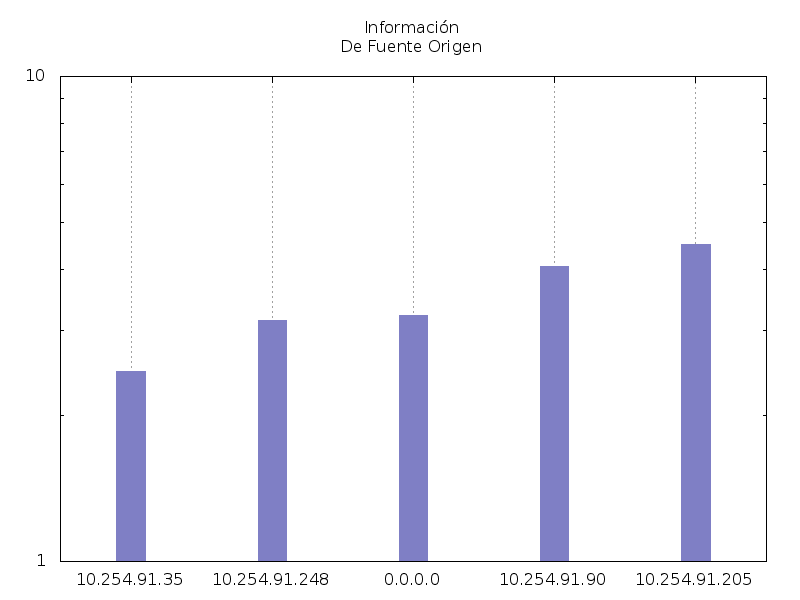
\includegraphics[width=0.5\textwidth]{img/graph/escenario_3/info_src.png}
\end{figure}


\begin{figure}[!ht]
    \centering
    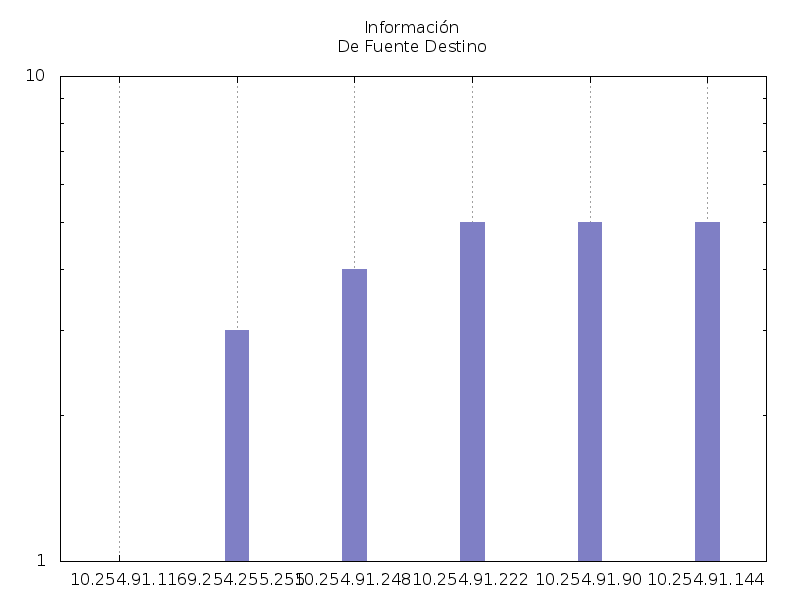
\includegraphics[width=0.5\textwidth]{img/graph/escenario_3/info_dst.png}
\end{figure}

	\par Tanto para este caso como sucedía con las probabilidades, estos son los valores mas significativos y podemos ver que como el router da una cantidad tan baja de informacion la entropia de $S_{src}$ sera mucho menor a la de $S_{dst}$.

	\par Efectivamente eso se da al calcular la media de la información:
    
\vspace{6 mm}

\begin{center}
\begin{tabular}{|c|c|}
\hline
Fuente $S$ & Entropía $H(S)$\\
\hline
$S_{src}$ & 4.96757\\
$S_{dst}$ & 2.8455\\
\hline
\end{tabular}
\end{center}

\subsection{Conclusiones Preliminares}

\par En base a lo visto podemos decir que mediante lo obtenido en la captura pudimos determinar los nodos distinguidos de esta red, al menos para este caso donde solo parece haber un router el símbolo de las fuentes con menor información coincidió con su dirección.


%\subsection{Subsection Heading Here}
%Subsection text here.

% needed in second column of first page if using \IEEEpubid
%\IEEEpubidadjcol

%\subsubsection{Subsubsection Heading Here}
%Subsubsection text here.


% An example of a floating figure using the graphicx package.
% Note that \label must occur AFTER (or within) \caption.
% For figures, \caption should occur after the \includegraphics.
% Note that IEEEtran v1.7 and later has special internal code that
% is designed to preserve the operation of \label within \caption
% even when the captionsoff option is in effect. However, because
% of issues like this, it may be the safest practice to put all your
% \label just after \caption rather than within \caption{}.
%
% Reminder: the "draftcls" or "draftclsnofoot", not "draft", class
% option should be used if it is desired that the figures are to be
% displayed while in draft mode.
%
%\begin{figure}[!t]
%\centering
%\includegraphics[width=2.5in]{myfigure}
% where an .eps filename suffix will be assumed under latex, 
% and a .pdf suffix will be assumed for pdflatex; or what has been declared
% via \DeclareGraphicsExtensions.
%\caption{Simulation Results.}
%\label{fig_sim}
%\end{figure}

% Note that IEEE typically puts floats only at the top, even when this
% results in a large percentage of a column being occupied by floats.
% However, the Computer Society has been known to put floats at the bottom.


% An example of a double column floating figure using two subfigures.
% (The subfig.sty package must be loaded for this to work.)
% The subfigure \label commands are set within each subfloat command,
% and the \label for the overall figure must come after \caption.
% \hfil is used as a separator to get equal spacing.
% Watch out that the combined width of all the subfigures on a 
% line do not exceed the text width or a line break will occur.
%
%\begin{figure*}[!t]
%\centering
%\subfloat[Case I]{\includegraphics[width=2.5in]{box}%
%\label{fig_first_case}}
%\hfil
%\subfloat[Case II]{\includegraphics[width=2.5in]{box}%
%\label{fig_second_case}}
%\caption{Simulation results.}
%\label{fig_sim}
%\end{figure*}
%
% Note that often IEEE papers with subfigures do not employ subfigure
% captions (using the optional argument to \subfloat[]), but instead will
% reference/describe all of them (a), (b), etc., within the main caption.


% An example of a floating table. Note that, for IEEE style tables, the 
% \caption command should come BEFORE the table. Table text will default to
% \footnotesize as IEEE normally uses this smaller font for tables.
% The \label must come after \caption as always.
%
%\begin{table}[!t]
%% increase table row spacing, adjust to taste
%\renewcommand{\arraystretch}{1.3}
% if using array.sty, it might be a good idea to tweak the value of
% \extrarowheight as needed to properly center the text within the cells
%\caption{An Example of a Table}
%\label{table_example}
%\centering
%% Some packages, such as MDW tools, offer better commands for making tables
%% than the plain LaTeX2e tabular which is used here.
%\begin{tabular}{|c||c|}
%\hline
%One & Two\\
%\hline
%Three & Four\\
%\hline
%\end{tabular}
%\end{table}


% Note that IEEE does not put floats in the very first column - or typically
% anywhere on the first page for that matter. Also, in-text middle ("here")
% positioning is not used. Most IEEE journals use top floats exclusively.
% However, Computer Society journals sometimes do use bottom floats - bear
% this in mind when choosing appropriate optional arguments for the
% figure/table environments.
% Note that, LaTeX2e, unlike IEEE journals, places footnotes above bottom
% floats. This can be corrected via the \fnbelowfloat command of the
% stfloats package.



%\section{Conclusion}
%The conclusion goes here.

\section{Conclusiones}\label{sec:conclusiones}
    \IEEEPARstart{LL}egados al final del trabajo expuesto, podemos decir que determinar valores 
de $\alpha$ y $\beta$ que acerquen la estimac\'ion del RTO al RTT ''real'' no es tarea sencilla.

En base a los resultados obtenidos mediante la primera m\'etrica que usamos, el RMSD, tener 
tantos valores variables en consideraci\'on nos genera un campo demasiado amplio de resultados.
A pesar de eso pudimos ver la relaci\'on directa que tienen los cambios introducidos al
protocolo (el delay y la probabilidad de dropeo) en la estimaci\'on del RTO como bien describimos
en la secci\'on de resultados.

Algo similar sucedi\'o al considerar la segunda m\'etrica de la experimentac\'on, el throughput,
a grandes rasgos no se consegu\'ia ver una relaci\'on clara entre la informaci\'on transmitida sin
errores y los valores de $\alpha$ y $\beta$ como s\'i suced\'ia con $\phi$ y $\delta$, los resultados 
obtenidos reflejaban como era de esperarse que a mayor delay menor era la eficiencia de la comunicac\'ion 
y que a mayor probabilidad de p\'erdida de paquete lo mismo suced\'ia.


Pero no fue hasta analizar enfonc\'andose en un entorno m\'as peque\~no de valores, esto es,
al fijar ciertos par\'ametros y concentrarnos en como repercut\'ian $\alpha$ y $\beta$, que pudimos 
determinar valores que consideramos eficientes de ellos dependiendo el caso.

A partir de las modificaciones hechas al protocolo, el estudio de distintas m\'etricas y formas de
presentar y analizar los resultados, se reduci\'o el tiempo que pudimos dedicarle a la experimentaci\'on
propiamente dicha, y quedaron pendientes posibles trabajos a realizar, uno de ellos es estudiar el
compromiso entre el RMSD y el throughput [AMPLIAR CON LO QUE ESTA EN PAG6.]

Otro punto que vale la pena destacar es que los resultados obtenidos dependen completamente de la 
implementaci\'on del protocolo, que consideramos no finalizada, ya que hubiese sido interesante
continuar modificando el c\'odigo a partir de los errores que llegamos a reportar en la secci\'on 
\ref{sec:experimento:dificultades}, pero no resolver completamente, lo cual nos hubiese permitido 
a su vez estudiar distintos entornos de experimentaci\'on y hacer un an\'alisis m\'as profundo de 
multiples casos posibles. Al continuar con esto, los resultados pueden llegar a variar y ser
menos vol\'atiles o irregulares que los que presentamos.

Como palabras finales sobre el trabajo hecho, consideramos que el estudio de la congesti\'on de TCP
es m\'as que interesante y el trabajo presentado nos permite ver en pr\'actica la importancia de varios 
conceptos de la capa de transporte y el control de congestion estudiados a lo largo de la cursada
de la materia.



% if have a single appendix:
%\appendix[Proof of the Zonklar Equations]
% or
%\appendix  % for no appendix heading
% do not use \section anymore after \appendix, only \section*
% is possibly needed

% use appendices with more than one appendix
% then use \section to start each appendix
% you must declare a \section before using any
% \subsection or using \label (\appendices by itself
% starts a section numbered zero.)
%


%\appendices
%\section{Proof of the First Zonklar Equation}
%Appendix one text goes here.

% you can choose not to have a title for an appendix
% if you want by leaving the argument blank
%\section{}
%Appendix two text goes here.


% use section* for acknowledgement
%\ifCLASSOPTIONcompsoc
  % The Computer Society usually uses the plural form
%  \section*{Acknowledgments}
%\else
  % regular IEEE prefers the singular form
%  \section*{Acknowledgment}
%\fi


%The authors would like to thank...


% Can use something like this to put references on a page
% by themselves when using endfloat and the captionsoff option.
\ifCLASSOPTIONcaptionsoff
  \newpage
\fi



% trigger a \newpage just before the given reference
% number - used to balance the columns on the last page
% adjust value as needed - may need to be readjusted if
% the document is modified later
%\IEEEtriggeratref{8}
% The "triggered" command can be changed if desired:
%\IEEEtriggercmd{\enlargethispage{-5in}}

% references section

% can use a bibliography generated by BibTeX as a .bbl file
% BibTeX documentation can be easily obtained at:
% http://www.ctan.org/tex-archive/biblio/bibtex/contrib/doc/
% The IEEEtran BibTeX style support page is at:
% http://www.michaelshell.org/tex/ieeetran/bibtex/
%\bibliographystyle{IEEEtran}
% argument is your BibTeX string definitions and bibliography database(s)
%\bibliography{IEEEabrv,../bib/paper}
%
% <OR> manually copy in the resultant .bbl file
% set second argument of \begin to the number of references
% (used to reserve space for the reference number labels box)
%\begin{thebibliography}{1}

%\bibitem{IEEEhowto:kopka}
%H.~Kopka and P.~W. Daly, \emph{A Guide to \LaTeX}, 3rd~ed.\hskip 1em plus
%  0.5em minus 0.4em\relax Harlow, England: Addison-Wesley, 1999.

%\end{thebibliography}

% biography section
% 
% If you have an EPS/PDF photo (graphicx package needed) extra braces are
% needed around the contents of the optional argument to biography to prevent
% the LaTeX parser from getting confused when it sees the complicated
% \includegraphics command within an optional argument. (You could create
% your own custom macro containing the \includegraphics command to make things
% simpler here.)
%\begin{IEEEbiography}[{\includegraphics[width=1in,height=1.25in,clip,keepaspectratio]{mshell}}]{Michael Shell}
% or if you just want to reserve a space for a photo:

%\begin{IEEEbiography}{Michael Shell}
%Biography text here.
%\end{IEEEbiography}

% if you will not have a photo at all:
%\begin{IEEEbiographynophoto}{John Doe}
%Biography text here.
%\end{IEEEbiographynophoto}

% insert where needed to balance the two columns on the last page with
% biographies
%\newpage

%\begin{IEEEbiographynophoto}{Jane Doe}
%Biography text here.
%\end{IEEEbiographynophoto}

% You can push biographies down or up by placing
% a \vfill before or after them. The appropriate
% use of \vfill depends on what kind of text is
% on the last page and whether or not the columns
% are being equalized.

%\vfill

% Can be used to pull up biographies so that the bottom of the last one
% is flush with the other column.
%\enlargethispage{-5in}



% that's all folks
\printbibliography
\end{document}
